\documentclass[a4paper,12pt]{article}

%\documentclass[a4paper,12pt, draft]{article}
\documentclass[a4paper,12pt]{article}

%%% Работа с русским языком
\usepackage{cmap}					% поиск в PDF
\usepackage{mathtext} 				% русские буквы в формулах
\usepackage[T2A]{fontenc}			% кодировка
\usepackage[utf8]{inputenc}			% кодировка исходного текста
\usepackage[english,russian]{babel}	% локализация и переносы
\usepackage{indentfirst}            % красная строка в первом абзаце
\frenchspacing                      % равные пробелы между словами и предложениями

%%% Дополнительная работа с математикой
\usepackage{amsmath,amsfonts,amssymb,amsthm,mathtools} % пакеты AMS
\usepackage{icomma}                                    % "Умная" запятая

%%% Свои символы и команды
\usepackage{centernot} % центрированное зачеркивание символа
\usepackage{stmaryrd}  % некоторые спецсимволы

\renewcommand{\epsilon}{\ensuremath{\varepsilon}}
\renewcommand{\phi}{\ensuremath{\varphi}}
\renewcommand{\kappa}{\ensuremath{\varkappa}}
\renewcommand{\le}{\ensuremath{\leqslant}}
\renewcommand{\leq}{\ensuremath{\leqslant}}
\renewcommand{\ge}{\ensuremath{\geqslant}}
\renewcommand{\geq}{\ensuremath{\geqslant}}
\renewcommand{\emptyset}{\ensuremath{\varnothing}}

\DeclareMathOperator{\sgn}{sgn}
\DeclareMathOperator{\ke}{Ker}
\DeclareMathOperator{\im}{Im}
\DeclareMathOperator{\re}{Re}

\newcommand{\N}{\mathbb{N}}
\newcommand{\Z}{\mathbb{Z}}
\newcommand{\Q}{\mathbb{Q}}
\newcommand{\R}{\mathbb{R}}
\newcommand{\Cm}{\mathbb{C}}
\newcommand{\F}{\mathbb{F}}
\newcommand{\id}{\mathrm{id}}
\newcommand{\imp}[2]{
	(#1\,\,$\ra$\,\,#2)\,\,
}
\newcommand{\System}[1]{
	\left\{\begin{aligned}#1\end{aligned}\right.
}
\newcommand{\Root}[2]{
	\left\{\!\sqrt[#1]{#2}\right\}
}
\newcommand{\RR}{\R}
\newcommand{\NN}{\N}
\renewcommand{\subseteq}{\subset}
\newcommand{\sub}{\subset}
\newcommand{\sconstr}{\;\vert\;}
\newcommand{\thus}{\implies}

\newcommand{\defeq}{\vcentcolon= }
\newcommand{\defev}{\stackrel{\Delta}{\Longleftrightarrow}}
\newcommand{\deriv}[3][1]{%
	\ifthenelse{#1>1}{%
		\frac{\dlta^{#1} {#2}}{\dlta {#3}^{#1}}
	}{%
		\frac{\dlta {#2}}{\dlta {#3}}
	}%
}

\renewcommand\labelitemi{$\triangleright$}

\let\bs\backslash
\let\lra\Leftrightarrow
\let\ra\Rightarrow
\let\la\Leftarrow
\let\emb\hookrightarrow

%%% Перенос знаков в формулах (по Львовскому)
\newcommand{\hm}[1]{#1\nobreak\discretionary{}{\hbox{$\mathsurround=0pt #1$}}{}}

%%% Работа с картинками
\usepackage{graphicx}    % Для вставки рисунков
\setlength\fboxsep{3pt}  % Отступ рамки \fbox{} от рисунка
\setlength\fboxrule{1pt} % Толщина линий рамки \fbox{}
\usepackage{wrapfig}     % Обтекание рисунков текстом

%%% Работа с таблицами
\usepackage{array,tabularx,tabulary,booktabs} % Дополнительная работа с таблицами
\usepackage{longtable}                        % Длинные таблицы
\usepackage{multirow}                         % Слияние строк в таблице

%%% Теоремы
\theoremstyle{plain}
\newtheorem{theorem}{Теорема}[section]
\newtheorem{lemma}{Лемма}[section]
\newtheorem{proposition}{Утверждение}[section]
\newtheorem*{exercise}{Упражнение}
\newtheorem*{problem}{Задача}

\theoremstyle{definition}
\newtheorem{definition}{Определение}[section]
\newtheorem*{corollary}{Следствие}
\newtheorem*{note}{Замечание}
\newtheorem*{reminder}{Напоминание}
\newtheorem*{example}{Пример}

\theoremstyle{remark}
\newtheorem*{solution}{Решение}

%%% Оформление страницы
\usepackage{extsizes}     % Возможность сделать 14-й шрифт
\usepackage{geometry}     % Простой способ задавать поля
\usepackage{setspace}     % Интерлиньяж
\usepackage{enumitem}     % Настройка окружений itemize и enumerate
\setlist{leftmargin=25pt} % Отступы в itemize и enumerate

\geometry{top=25mm}    % Поля сверху страницы
\geometry{bottom=30mm} % Поля снизу страницы
\geometry{left=20mm}   % Поля слева страницы
\geometry{right=20mm}  % Поля справа страницы

\setlength\parindent{15pt}        % Устанавливает длину красной строки 15pt
\linespread{1.3}                  % Коэффициент межстрочного интервала
%\setlength{\parskip}{0.5em}      % Вертикальный интервал между абзацами
%\setcounter{secnumdepth}{0}      % Отключение нумерации разделов
%\setcounter{section}{-1}         % Нумерация секций с нуля
\usepackage{multicol}			  % Для текста в нескольких колонках
\usepackage{soulutf8}             % Модификаторы начертания
\mathtoolsset{showonlyrefs=true} % показывать номера формул только у тех, у которых есть ссылки по eqref
%%% Содержаниие
\usepackage{tocloft}
\tocloftpagestyle{main}
%\setlength{\cftsecnumwidth}{2.3em}
%\renewcommand{\cftsecdotsep}{1}
%\renewcommand{\cftsecpresnum}{\hfill}
%\renewcommand{\cftsecaftersnum}{\quad}

%%% Шаблонная информация для титульного листа
\newcommand{\CourseName}{Математический анализ}
\newcommand{\FullCourseNameFirstPart}{\so{Введение в математический анализ}}
\newcommand{\SemesterNumber}{I}
\newcommand{\LecturerInitials}{Гусев Николай Анатольевич}
\newcommand{\CourseDate}{осень 2022}
\newcommand{\AuthorInitials}{Копанов Антон}
\newcommand{\AuthorInitialssecond}{Клищ Данил}
\newcommand{\VKLink}{https://vk.com/notnako}
\newcommand{\GithubLink}{https://github.com/MIPT-Group/Lectures_Tex_Club}
\newcommand{\VKLinksecond}{https://vk.com/dan.klishch}

%%% Колонтитулы
\usepackage{titleps}
\newpagestyle{main}{
	\setheadrule{0.4pt}
	\sethead{\CourseName}{}{\hyperlink{intro}{\;Назад к содержанию}}
	\setfootrule{0.4pt}                       
	\setfoot{ФПМИ МФТИ, \CourseDate}{}{\thepage} 
}
\pagestyle{main}  

%%% Нумерация уравнений
\makeatletter
\def\eqref{\@ifstar\@eqref\@@eqref}
\def\@eqref#1{\textup{\tagform@{\ref*{#1}}}}
\def\@@eqref#1{\textup{\tagform@{\ref{#1}}}}
\makeatother                      % \eqref* без гиперссылки
\numberwithin{equation}{section}  % Нумерация вида (номер_секции).(номер_уравнения)
\mathtoolsset{showonlyrefs= true} % Номера только у формул с \eqref{} в тексте.

%%% Гиперссылки
\usepackage{hyperref}
\usepackage[usenames,dvipsnames,svgnames,table,rgb]{xcolor}
\hypersetup{
	unicode=true,            % русские буквы в раздела PDF
	colorlinks=true,       	 % Цветные ссылки вместо ссылок в рамках
	linkcolor=black!15!blue, % Внутренние ссылки
	citecolor=green,         % Ссылки на библиографию
	filecolor=magenta,       % Ссылки на файлы
	urlcolor=NavyBlue,       % Ссылки на URL
}

%%% Графика
\usepackage{tikz}        % Графический пакет tikz
\usepackage{tikz-cd}     % Коммутативные диаграммы
\usepackage{tkz-euclide} % Геометрия
\usepackage{stackengine} % Многострочные тексты в картинках
\usetikzlibrary{angles, babel, quotes}

%%% Всю шаблонную информацию можно менять тут
\newcommand{\FullCourseNameFirstPart}{\so{ТЕОРИЯ~ФУНКЦИЙ}}
\newcommand{\FullCourseNameSecondPart}{\so{КОМПЛЕКСНОГО~ПЕРЕМЕННОГО}}
\newcommand{\SchoolName}{ФПМИ}
\newcommand{\TrackName}{ПМФ}
\newcommand{\SemesterNumber}{V}
\newcommand{\LecturerInitials}{Половинкин Евгений Сергеевич}
\newcommand{\AutherInitials}{Маланчук София}
\newcommand{\VKLink}{https://vk.com/smalanchuk0}
\newcommand{\OverleafLink}{https://www.overleaf.com/read/vgjwvzdrzvqc}
\newcommand{\GithubLink}{https://github.com/MIPT-Group/Lectures_Tex_Club/}
\newcommand{\CourseName}{ТФКП} %  Используется в преамбуле для создания названия предмета в верхнем контитуле   
\newcommand{\CourseDate}{Осень 2020}           %  Используется в преамбуле для создания даты в нижнем контитуле

%\includeonly{lectures/lect05,lectures/lect06}  % Чтобы скомпилировать только часть лекций

\begin{document}
    %%% Всю шаблонную информацию можно менять тут
\newcommand{\FullCourseNameFirstPart}{\so{ТЕОРИЯ ГРУПП}}
\newcommand{\SemesterNumber}{III}
\newcommand{\LecturerInitials}{Богданов Илья Игоревич}
\newcommand{\AutherInitials}{Даниил Дрябин}
\newcommand{\VKLink}{https://vk.com/ax_equals_b}
\newcommand{\GithubLink}{https://github.com/daniild71r/lectures_tex_club}

\begin{titlepage}
	\clearpage\thispagestyle{empty}
	\centering
	
	%\textit{Федеральное государственное автономное учреждение \\
	%	высшего профессионального образования}
	%\vspace{0.5ex}
	
	%\textbf{Московский Физико-Технический Институт \\ КЛУБ ТЕХА ЛЕКЦИЙ}
	\textbf{Московский физико-технический институт \\ Физтех-школа прикладной математики и информатики}
	\vspace{20ex}
	\vspace{13ex}
	
	{\textbf{\FullCourseNameFirstPart}}
	
	\SemesterNumber\ СЕМЕСТР  
	\vspace{1ex}
	
	Лектор: \textit{\LecturerInitials}
	
	\begin{figure}[!ht]
		\centering
		
\includegraphics[width=0.4\textwidth]{images/logo_ltc.png}
	\end{figure}

	\begin{flushright}
		\noindent
		Автор 2020: \href{\VKLink}{\textit{\AutherInitials}}
		\\
		Дополнил 2022: \textit{Даниил Максимов}
		\\
		\href{\GithubLink}{\textit{Проект на Github}}
	\end{flushright}
	
	\vfill
	\CourseDate
	\pagebreak
\end{titlepage}

    \hypertarget{intro}{}
    \tableofcontents
    \newpage
    \section{Unix системы}

\subsection{Компоненты операционной системы}

\begin{Def}
	\underline{Ядро} --- программа, которая запускается самой первой. Имеет привилегированное положение на процессоре и может взаимодействовать с <<железом>> напрямую.
\end{Def}

\begin{Def}
	\underline{Базовые библиотеки}: зачастую входят в состав операционной системы, потому что привязаны к определенному ядру (версии ядра), чтобы максимально использовать его функциональность. 
\end{Def}

\begin{Def}
\underline{Служебные сервисы} --- ведение логов, обработка сетевых соединения, и т.д.
\end{Def}

\begin{Def}
\underline{Минимальная пользовательская оболочка} --- чтобы пользователь мог взаимодействовать с системой.
\end{Def}

\subsection{Процессы}

\begin{Def}
\underline{Процесс} --- любой экземпляр программы, работающей в операционной системе.
\end{Def}

Примеры:
\begin{itemize}
	\item Приложения
	\item Фоновые сервисы (демоны)
	\item Команды в терминале
\end{itemize}

Главные команды для мониторинга процессов:
\begin{itemize}
	\item ps -A -- список процессов
	\item pstree -- иерархия процессов
	\item top
\end{itemize}

\subsection{UNIX программы}

Программы:
\begin{itemize}
	\item \textbf{Бинарные исполняемые файлы.}
	\item \textbf{Текстовый файл, начинающийся с \#!.} После \#! указывается путь к интерпретатору (например, \#!/bin/bash). Это могут быть скрипты на Python/Perl/Escript или Shell скрипт.
\end{itemize}

Название файла и его расширение не имеет значения. Любой файл, имеющий атрибут 
<<исполняемый>> является программой.

\subsection{UNIX пользователи}

Единственные привилегированный пользователь: root (UID = 0).

Непривилегерованные пользователи:
\begin{itemize}
	\item Реальные пользователи, которые могут войти в систему (UID $\ge$ 1000)
	\item Фейковые пользователи, привязанные к сервисам (UID $<$ 1000).
\end{itemize}

\textbf{Зачем сервисам нужны фейковые пользователи?}
Допустим, у вас есть веб-сервер и сервер баз данных. Теоретически какой-то пользователь
может подключиться к веб-серверу и найти там уязвимость. Для того, чтобы 
минимизировать возможный ущерб от уязвимости в одном из процессов, процессы запускаются
под разными пользователями и не имеют права общаться друг с другом.

Непривилегерованные пользователи могут временно получить 
дополнительные привилегии:

\begin{itemize}
	\item su - запускает терминал от имени root
	\item sudo - запускает любую программу от имени root
	\item Запустить программу с атрибутом SUID и владельцем root. SUID атрибут означает, что при запуске программа
	исполняется от того пользователя, кто является владельцем файла. Кстати, так и 
	работает команда sudo, владелец sudo - root, а также у sudo проставлен атрибут SUID.
	\item Запустить программу с <<capabilities>> флагами. Эти флаги позволяют тонко настроить, что можно делать программе, а что - нельзя.
\end{itemize}

\subsection{UNIX межпроцессорное взаимодействие}

Процессы работают изолированно друг от друга. Единственный способ взаимодействовать друг с другом --- использовать методы межпроцессорного взаимодействия ядра (Inter-Process Communication, IPC):

\begin{itemize}
	\item {Сигналы} для коротких сообщений
	\item {Каналы и сокеты} для последовательных данных
	\item {Разделяемая память}, в которой хранятся большие куски данных
\end{itemize}

\subsection{Процесс запуска}

\begin{enumerate}
	\item {Загрузчик} с диска или UEFI материнской платы выполняется в привилегированном режиме
	\item Загрузчик запускает {ядро}, тоже в привилегированном режиме.
	\item Ядро запускает первый непривелигерованный процесс: {init или systemd}.
\end{enumerate}

\subsection{Сервисы (``Демоны'')}

\begin{Def}
	\underline{Сервисы} --- это специальные системные службы, которые работают в фоновом режиме.
\end{Def}

\newpage

Минимальный сет во многих системах:

\begin{itemize}
	\item \textbf{dhclient} -- держит активным полученный IP адрес в сети
	\item \textbf{getty} -- переключение между графическим/консольным входом в систему
	\item \textbf{sshd} -- подключение по ssh
	\item \textbf{ntpd или chronyd} -- синхронизация времени
	\item \textbf{syslogd} -- системный лог
\end{itemize}

\subsection{\#!/bin/sh}

В терминале вы работаете в интерпретаторе \texttt{shell}. \texttt{shell} предоставляет возможность выполнять
команды и последовательности команд.

Бывают разные интерпретаторы \texttt{shell}:
\begin{itemize}
	\item самодостаточный \texttt{shell} program: \textbf{FreeBSD}
	\item основной в \texttt{Linux}: \textbf{bash}
	\item debian: \textbf{dash}
	\item alpine: \textbf{busybox}
	\item maxOS X: \textbf{zsh}
\end{itemize}

\subsection{Системный демон (systemd)}
\begin{Def}
Процесс, который управляет всеми остальными процессами. При этом сам является обычным процессом. \texttt{Systemd} пришел на замену INIT-процессу.

\end{Def}

Чем systemd лучше?
\begin{itemize}
	\item Устранение интерпретации \texttt{shell} скриптов. 
	\item Запуск сервисов параллельно
\end{itemize}

\subsubsection{Концепты systemd}

\begin{itemize}
	\item Сервисы
	\item Цели:
		\begin{itemize}
			\item \underline{Стандартные цели}. Например, уровни \texttt{init} в System-V:
				\begin{itemize}
					\item poweroff.target (init 0)
					\item rescue.target (init 1)
					\item multi-user.target (init 3)
					\item graphical.target (init 5)
					\item reboot.target (init 6)
					\item sleep.target и hibertate.target (не присутствуют в System-V)
				\end{itemize}
			\item \underline{Специальные цели}
		\end{itemize}
\end{itemize}

\subsection{Фоновые задачи}

\begin{itemize}
	\item \textbf{Нет привязанного к задаче терминала.} Для того, чтобы сигнал \texttt{SIGHUP}
	не останавливал исполнение задачи используется команда \texttt{nohup}.
	\item \textbf{Пишут в лог.} Иногда пишут данные в какую-то старинную 
	локальную почтовую систему.
	\item \textbf{Запускается в единственном экземпляре.} Обычно это достигается
	с помощью file lock.
\end{itemize}

\subsection{Дистрибутивы \texttt{Linux}}

Ядро называется Linux. Базовая система --- минимальная юзабельная система.

\underline{Дистрибутив}:
\begin{itemize}
	\item Ядро
	\item Базовая система
	\item GUI оболочка
	\item Программное обеспечение 
\end{itemize}

\subsubsection{Какие есть дистрибутивы?} 

Общего назначения:
\begin{itemize}
	\item OpenSUSE
	\item Fedora
	\item Debian
	\item Ubuntu
\end{itemize}

Специфические дистрибутивы:
\begin{itemize}
	\item Alpine Linux --- очень легковесный, поэтому его
	хорошо ставить на виртуальную машину.
	\item Kali Linux --- используется для тестов на безопасность.
\end{itemize}


    \begin{flushright}
    \textit{Лекция 2 (от 08.09)}
\end{flushright}
\section{$\S 3.$ Дифференцирование}
Пусть $z_0 \in \CC$, $B_r(z_0)$ и $f: B_r(z_0) \mapsto \CC$
\Def
Пусть $f: B_r(z_0) \mapsto \CC$. Если
\begin{equation}\label{(3.1)}
    \exists \dst \lim_{z \mapsto z_0} \frac{f(z)-f(z_0)}{z-z_0}
\end{equation}
то он называется \textbf{производной функции $f$ в точке $z_0$} (записывается
$f'(z_0)$).
\\
Можем расписать предел:
\begin{equation}\label{(3.2)}
    \forall \varepsilon > 0 \ \exists \delta(\varepsilon)>0: \ z \in B_\delta(z_0), \ \left| \frac{f(z) - f(z_0)}{z-z_0} - f'(z_0) \right| < \varepsilon
\end{equation}
\begin{equation}\label{(3.3)}
    f(z) = f(z_0) + f'(z_0)(z-z_0) + \alpha(z-z_0)
\end{equation}
\begin{equation}\label{(3.4)}
    \lim_{z \to z_0}\frac{\alpha(z-z_0)}{z-z_0} = 0
\end{equation}
\begin{align*}
  & f(z_0) = u(x,y) + iv(x,y)
\end{align*}
\Def
Говорят, что $f: B_r(z_0) \mapsto \CC$ \textbf{дифференцируема в точке $z_0$},
если
\begin{equation}\label{(3.5)}
    \exists A \in \CC: \ f(z) = f(z_0)+A(z-z_0)+o(z-z_0)
\end{equation}
\lemma
$f: B_r(z_0) \mapsto \CC$ дифференцируема в $z_0$ $\Leftrightarrow$ $\exists
f'(z_0)$, $A = f'(z_0)$
\pr
Очевидно.
\\
Обозначим: $\Delta x = x-x_0$, $\Delta y = y - y_0$, $\Delta z = z-z_0 = \Delta
x + i \Delta y$, $\Delta u = u(x,y)-u(x_0,y_0)$, $\Delta v = v(x,y)-v(x_0,y_0)$,
$\Delta f = f(x,y)-f(x_0,y_0) = \Delta u + i \Delta v$.
\theorem
$f: B_r(z_0) \mapsto \CC$ дифференцируема в $z_0$ т огда и только тогда, когда
\begin{itemize}
    \item $u(x,y)$, $v(x,y)$ дифференцируемы в $(x_0,y_0)$ (в $\RR^2$)
    \item выполняется условие Коши-Римана (УКР):
    \begin{equation}\label{(3.6)}
        \begin{cases}
            \dst \frac{\partial u}{\partial x} = \dst \frac{\partial v}{\partial y} \\
            \dst \frac{\partial v}{\partial x} = - \dst \frac{\partial u}{\partial y}
        \end{cases}
        % \left\{ \begin{matrix}
        %         \dst \frac{\partial u}{\partial x} = \dst \frac{\partial v}{\partial y} \\
        %         \dst \frac{\partial v}{\partial x} = - \dst \frac{\partial u}{\partial y}
        %     \end{matrix} \right.
    \end{equation}
\end{itemize}
При этом
\begin{equation}\label{(3.7)}
    f'(z_0) = \frac{\partial u}{\partial x}(x_0,y_0) + i\frac{\partial v}{\partial x}(x_0,y_0) = \frac{\partial v}{\partial y}(x_0,y_0) - i\frac{\partial u}{\partial y}(x_0,y_0)
\end{equation}
\pr
Докажем в обе стороны.
\begin{itemize}
    \item Необходимость.
    \begin{align*}
      & \exists f'(z_0) = a+ib = A \in \CC
    \end{align*}
    Значит, по определению дифференцируемости
    \begin{align*}
      & \Delta f = A \Delta z + \alpha(\Delta z); \ \alpha(\Delta z) = \alpha_1(\Delta x, \Delta y) + i\alpha_2(\Delta x, \Delta y)
    \end{align*}
    \begin{align*}
      & \left\{ \begin{matrix}
              \Delta u = a \Delta x - b \Delta y + \alpha_1(\Delta x, \Delta y) \\
              \Delta v = b \Delta x + a \Delta y + \alpha_2(\Delta x, \Delta y)
          \end{matrix} \right.
    \end{align*}
    \begin{align*}
      & \left| \alpha_1 \right| \leq \left| \alpha \right|, \ \left| \alpha_2 \right| \leq \left| \alpha \right|
    \end{align*}
    \begin{align*}
      & \lim_{(\Delta x; \Delta y) \to (0;0)}\left( \frac{\left| \alpha_1(\Delta x, \Delta y) \right|}{\sqrt{\left( \Delta x \right)^2 + \left( \Delta y \right)^2}} \right) \leq \lim_{\Delta z \to 0}\left( \frac{\left| \alpha(\Delta z) \right|}{\left| \Delta z \right|} \right) = 0
    \end{align*}
    Значит, $u$ дифференцируема, причем $\dst \frac{\partial u}{\partial x} =
    a$, $\dst \frac{\partial u}{\partial y} = -b$.
    \\
    Аналогично для $v$, причем $\dst \frac{\partial v}{\partial x} = b$, $\dst
    \frac{\partial v}{\partial y} = a$.
    \\
    Видим выполнимость УКР.
    \\
    Выполнимость \eqref{(3.7)} очевидна.
    \item Достаточность.
    \\
    Пусть $u$, $v$ дифференцируемы в $(x_0,y_0)$ и выполняется УКР. Тогда
    \begin{align*}
      & \Delta f = \Delta u + i \Delta v = \frac{\partial u}{\partial x} \Delta x + \frac{\partial u}{\partial y} \Delta y + \alpha_1(\Delta x, \Delta y) + i \left( \frac{\partial v}{\partial x} \Delta x + \frac{\partial v}{\partial y} \Delta y + \alpha_2(\Delta x, \Delta y)\right) = \\
      & \frac{\partial u}{\partial x} \Delta x - \frac{\partial v}{\partial x} \Delta y + \alpha_1(\Delta x, \Delta y) + i \left( \frac{\partial v}{\partial x} \Delta x + \frac{\partial u}{\partial x} \Delta y + \alpha_2(\Delta x, \Delta y)\right) = \left( \frac{\partial u}{\partial x} + i \frac{\partial v}{\partial x}\right)\cdot \\
      & \cdot \left( \Delta x + i \Delta y \right)+ \alpha_1(\Delta x, \Delta y) + i \alpha_2(\Delta x, \Delta y)
    \end{align*}
    Значит,
    \begin{align*}
      & \exists f'(z_0) = \frac{\partial u}{\partial x} + i \frac{\partial v}{\partial x}
    \end{align*}
\end{itemize}
\Example
\begin{align*}
  & w = z^2
\end{align*}
\begin{itemize}
    \item[I] Найдем производную по определению.
    \begin{align*}
      & \frac{\Delta w}{\Delta z} = \frac{\left( z_0-\Delta z \right)^2 - z_0^2}{\Delta z} = \frac{2z_0\Delta z + \left( \Delta z \right)^2}{\Delta z} = 2z_0 + \Delta z \us{\Delta z \to 0}{\to} 2z_0
    \end{align*}
    \item[II] Найдем производную с использованием теоремы.
    \begin{align*}
      & z^2 = x^2-y^2+2ixy \Rightarrow u = x^2-y^2, \ v = 2xy
    \end{align*}
    \begin{align*}
      & u_x = 2x = v_y; \ u_y = -2y = - v_x
    \end{align*}
    Видим выполнимость УКР, поэтому
    \begin{align*}
      & w' = u_x+iv_x = 2x + 2iy = 2z
    \end{align*}
\end{itemize}
\Example
\begin{align*}
  & w = \left| z \right|^2
\end{align*}
\begin{align*}
  & \left| z \right|^2 = x^2+y^2 \Rightarrow u = x^2+y^2, \ v = 0
\end{align*}
\begin{align*}
  & u_x = 2x \neq 0 = v_y; \ u_y = 2y \neq 0 = - v_x
\end{align*}
(за исключением точки $(0;0)$). Видим выполнение УКР только в точке $(0;0)$, а
значит, и функция дифференцируема только в этой точке (с производной, равной
$0$).
\Example
\begin{align*}
  & w = \ol{z}
\end{align*}
\begin{align*}
  & \ol{z} = x - iy \Rightarrow u = x, \ v = -y
\end{align*}
\begin{align*}
  & u_x = 1 \neq -1 = v_y; \ u_y = 0 = - v_x
\end{align*}
Видим, что УКР не выполняется ни в одной точке $\CC$, а значит, функция нигде не
дифференцируема.
\prop
Если $f(z)$, $g(z)$ дифференцируемы, то:
\begin{itemize}
    \item дифференцируема и сумма:
    \begin{align*}
      & \left( f+g \right)' = f'+g'
    \end{align*}
    \item дифференцируемо и произведение:
    \begin{align*}
      & \left( fg \right)' = f'g+fg'
    \end{align*}
    \item дифференцируемо и частное (когда $g(z) \neq 0$):
    \begin{align*}
      & \left( \frac{f}{g} \right)' = \frac{f'g+fg'}{g^2}
    \end{align*}
\end{itemize}
\pr
Доказательства легко провести через УКР с использованием действительного
анализа.
\section{$\S 4.$ Регулярные и гармонические функции}
\example
$B_r(z_0)$~--- односвязная область как в $\CC$, так и в $\CCC$.
\example
$K = \left\{ z: 0 < r_1 < \left| z \right| < r_2 < \infty \right\}$~--- не
односвязная область ни в $\CC$, ни в $\CCC$.
\example
$B_r(\infty)$~--- односвязная область в $\CCC$, но не в $\CC$.
\Def
Если $u:G \mapsto \RR^1$, $G \subseteq \RR^2$~--- область, $u \in C^2(G)$,
$\Delta u = 0$, где $\Delta = \dst \frac{\partial^2}{\partial x^2} + \dst
\frac{\partial^2}{\partial y^2}$, то $u$ называется \textbf{гармонической}.
\Def ~
\begin{itemize}
    \item[а)]$f: G \mapsto \CC$, где $G \subseteq \CC$~--- область, называется
    \textbf{регулярной} (аналитической, голоморфной), если $\forall z \in G \
    \exists f'(z)$ (если $f$ дифференцируема в каждой точке $G$).
    \item[б)]$f: G \mapsto \CC$, $G \subseteq \CC$ называется
    \textbf{регулярной в точке $z_0 \in G$}, если $\exists r > 0: B_r(z_0)
    \subseteq G$, $f$ регулярна на $B_r(z_0)$.
\end{itemize}
\Def
Функция, заданная на произвольном множестве, \textbf{регулярна} на нем, если она
регулярна в каждой его точке.
\Example
\begin{align*}
  & w = z^n, \ n \geq 2, \ n \in \NN
\end{align*}
Производная существует в любой точке:
\begin{align*}
  & \frac{\left( z+\Delta z \right)^n - z^n}{\Delta z} = \frac{nz^{n-1}\Delta z + \left( \Delta z \right)^2\left( P(z, \Delta z) \right)}{\Delta z} \us{\Delta z \to 0}{\to} nz^{n-1}
\end{align*}
Значит, функция всюду дифференцируема и регулярна на всей $\CC$.
\\
Аналогично можно доказать регулярность всех многочленов и рациональных функций.
\Def
\begin{align*}
  & e^z = e^x\left( \cos y + i \sin y \right), \ z = x+iy
\end{align*}
Функция периодична с периодом $2 i \pi$; ее компоненты $u = e^x \cos y$, $v =
e^x \sin y$.
Выполняются УКР:
\begin{align*}
  & \begin{cases}
      u_x = e^x \cos y = v_y \\
      v_x = e^x \sin y = -u_y
  \end{cases}
  & % \left\{ \begin{matrix}
    %       u_x = e^x \cos y = v_y \\
    %       v_x = e^x \sin y = -u_y
    %   \end{matrix} \right.
\end{align*}
Значит, $f'(z) = u_x + iv_x = u+iv = e^z$ (аналогично $(e^{iz})' = ie^{iz}$,
$(e^{-iz})' = -ie^{iz}$).
\\
Эти функции всюду дифференцируемы, а значит, и регулярны.
\Def
Тригонометрические функции:
\begin{align*}
  & \cos z = \frac{e^{iz} + e^{-iz}}{2}, \ \sin z = \frac{e^{iz} -e^{-iz}}{2i}
\end{align*}
Для них выполняются известные свойства тригонометрических функций:
\begin{align*}
  & \cos^2 z + \sin^2 z = 1
\end{align*}
\begin{align*}
  & \sin(z_1+z_2) = \sin z_1 \cos z_2 + \sin z_2 \cos z_1, \ \cos(z_1+z_2) = \cos z_1 \cos z_2 - \sin z_1 \sin z_2
\end{align*}
\begin{align*}
  & \left( \sin z \right)' = \cos z, \ \left( \cos z \right)' = - \sin z
\end{align*}
Но ограниченность не выполняется.
\\
Раскроем функцию через $x$ и $y$.
\begin{align*}
  & \sin z = \sin(x+iy) = \sin x \cos iy + \cos x \sin iy = \sin x \ch y + i \cos x \sh y \\
  & \Downarrow \\
  & u(x,y) = \sin x \ch y, \ v = \cos x \sh y
\end{align*}
Тогда
\begin{align*}
  & \left| \sin z \right| = \sqrt{\sin^2 x \ch^2 y + \cos^2 x \sh^2 y} = \sqrt{(1-\cos^2 x)\ch^2 y + (\ch^2 y - 1)\cos^2 x} = \\
  & = \sqrt{\ch^2 y - \cos^2 x} \us{y \to \infty}{\sim} \ch x \us{y \to \infty}{\to} \infty
\end{align*}
\theorem
Пусть $f: G \mapsto \CC$ регулярна в $G$, $f = u + iv$, $u,v \in C^2(G)$. Тогда
$u$ и $v$ являются гармоническими.
\pr
\begin{align*}
  & \Delta u = \frac{\partial}{\partial x}\left( \frac{\partial u}{\partial x} \right)+ \frac{\partial}{\partial y} \left( \frac{\partial u}{\partial y} \right) = \frac{\partial^2 v}{\partial x \partial y} - \frac{\partial^2 v}{\partial y \partial x} = 0
\end{align*}
Переход объясняется условием Коши-Римана для регулярной $f$.
\\
Аналогично можно доказать гармоничность $v$.
\\
Пара функций, связанных УКР, называется \textbf{сопряженными гармоническими}.
\theorem
Пусть $G$~--- односвязная область, $u: G \mapsto \RR$ гармоническая. Тогда
сущетвует регулярная $f$, такая, что $\Real f(z) = u(x,y)$.
\pr
Пусть
\begin{align*}
  & P(x,y) = -\frac{\partial u}{\partial y}, \ Q(x,y) = \frac{\partial u}{\partial x}
\end{align*}
Хотим найти $v$, такую, что
\begin{align*}
  & \begin{cases}
      \dst \frac{\partial v}{\partial x} = P(x,y) \\
      \dst \frac{\partial v}{\partial y} = Q(x,y) 
      \end{cases}
\end{align*}
(из УКР на $f$).
\begin{align*}
  & dv = Pdx+Qdy
\end{align*}
Для односвязной $G$ и потенциального векторного поля $(P,Q)$, т.~е. такого, что
выполняется условие:
\begin{align*}
  & \frac{\partial P}{\partial x} -\frac{\partial Q}{\partial x}' = - \frac{\partial^2 u}{\partial y^2} - \frac{\partial^2 u}{\partial x^2} = 0
\end{align*}
В таком случае
\begin{align*}
  & v(x,y) = \int_{(x_0,y_0)}^{(x,y)} P dx + Q dy + const
\end{align*}
Полученая функция $v$ гармоническая. тогда $f(z) = u+iv$ будет регулярной в
каждой точке $G$.
\\
Аналогично можно построить регулярную функцию $f$ по данной гармонической $v$.
\Example
Пусть
\begin{align*}
  & u = xy, \ \Delta u = 0
\end{align*}
Значит, $u$ гармоническая. УКР:
\begin{align*}
  & v_x = -u_y = -x \Rightarrow v(x,y) = \frac{-x^2}{2} + \varphi(y)
\end{align*}
\begin{align*}
  & v_y = u_x = y \Rightarrow v(x,y) = \frac{-x^2}{2} + \frac{y^2}{2} + C
\end{align*}
Значит,
\begin{align*}
  & \varphi'(y) = y = v_y
\end{align*}
Тогда
\begin{align*}
  & v(x,y) = \frac{y^2-x^2}{2} + C
\end{align*}
Значит,
\begin{align*}
  & f(x,y)= xy+i\left( \frac{y^2-x^2}{2} + C \right) = -\frac{i}{2} \left( x^2-y^2+2ixy \right) + iC = -\frac{iz}{2} + iC
\end{align*}

    \section{Целочисленная арифметика}

\subsection{Уровни абстракции <<железа>>}
\begin{itemize}
    \item <<p>> и <<n>> полупроводники, проводники, конденсаторы и резисторы
    \item Транзисторы и диоды
    \item Логические элементы
    \item Арифметическо-логические юниты
    \item Центральный процессор
    \item Компьютерная система
\end{itemize}

Компьютер состоит из элементарных блоков, из которых строятся электрические
элементы. Они в свою очередь образуют логические элементы.

Ключевая часть компьютера - центральный процессор. А главная часть ЦП - арифметическо-логический блок, который выполняет все вычисления.

\subsection{Типы сигналов}

\begin{Def}
    \underline{Сигналы} --- это изменения напряжения в электрической сети. Их можно регистрировать
и дальше обрабатывать.
\end{Def}

Сигналы бывают двух видов:
\begin{itemize}
    \item \textbf{Аналоговый.} Сила сигнала изменяется непрерывно с изменением напряжения.
    \item \textbf{Цифровой.} Есть всего два состояния - высокий, либо низкий.
\end{itemize}


\subsection{Дискретные сигналы}

\begin{itemize}
    \item \textbf{Логический <<0>>.} Все, что ниже определенного значения
        напряжения --- это нулевой уровень.
    \item \textbf{Логическая <<1>>.}
    \item \textbf{Неопределенное состояние.} Напряжение между 0 и 1, не приводящее к изменению состояния.
    \item \textbf{Hi-Z состояние.} Физически какой-то контакт внутри процессора отключается от общей схемы, чтобы не оказывать влияние на все остальные компоненты.
\end{itemize}

\subsection{Арифметико-логический юнит}

Базовый юнит центрального процессора для реализации операций над числами:
\begin{itemize}
	\item Битовая логика
	\item Побитовые сдвиги
	\item Сложение и вычитание
	\item Умножение и деление
\end{itemize}

 Управление ходом программы --- тоже арифметические операции. 
 
 \subsection{Представление чисел и переполнения}
 Было на семинарах...
 
 \subsection{Значения из нескольких байтов}
 
 \begin{itemize}
 	\item Минимальный адресуемый обьем данных --- 8 бит.
 	\item За один такт процессора он может адресовать одно \textbf{машинное слово} процессора - 32 или 64 бита.
 \end{itemize}

\subsection{Big-Endian и Little-Endian}

\begin{itemize}
	\item \textbf{Big-Endian:}
	Выглядит как человеческое представление байтов.
	сначала старшие байты, потом - младшие
	Пример: большинство RISC процессоров по умолчанию.
	\item \textbf{Little-Endian:}
	сначала младшие байты, потом старшие
	Пример: Процессоры Intel и ARM.
\end{itemize}

\subsection{Ковертирование endian-ов}

Беззнаковые типы можно конвертировать просто побитовыми сдвигами. Достаточно переставить байты в обратном порядке.

Со знаковыми типами есть проблемы, потому что там первый бит отвечает за знак.

\subsection{Упаковка структур}

Размер любой структуры должен быть кратек размеру машинного слова. Это связано с тем оптимизацией времени чтения/записи. 

Поэтому если в структурке хранится два поля - на 16 бит и на 8 бит, то стуктура будет занимать 32 бита, а не 16 + 8 = 24. Ведь размер машинного слова в x86 равен 32 битам.

Если же прописать у структуры специальный атрибут, компилятор уложит поля вплотную.

\subsection{Где используется атрибут packed?}

\begin{itemize}
	\item Бинарные данные
	\item Сетевые пакеты
	\item Драйвера
\end{itemize}

В остальных случаях использование packed ненужно и даже вредно.

    \section{Команды процессора}

\subsection{Процессор}

Процессор умеет только манипулировать с целыми числами. Значение адреса - тоже число.

\subsection{Процессор с точки зрения пользователя}

У процессора есть:
\begin{itemize}
	\item Регистры - eax, ebx, ...
	\item Флаги - ZF, CF, SF
	\item Указатель на текущую команду (PC - pointer count)
\end{itemize}

\subsection{Команды x86}

nop - 0x00
halt - 0x10
call Dest - 0x80, Dest - 5 байтов
...

Команды кодируются переменным количеством байт. Количество байт может доходить до 6.

\subsection{Представление структур программы в виде простых инструкций}

Было на семинарах, на ассембелере писать уже должны уметь...

\subsection{CISC}

\begin{Def}
	\underline{CISC} --- \textbf{C}omplex \textbf{I}nstruction \textbf{S}et \textbf{C}omputing
\end{Def}

Процессоры: x86, Z80, PDP-11/VAX

Это тип архитектуры процессора, где:
\begin{itemize}
	\item Команд много, на все случаи жизни
	\item Кодируются переменным количеством байт
	\item Разные режимы адресации
	\item Упрощают жизнь программисту на ассемблере
\end{itemize}

Например, инструкция \textbf{loop} Address позволяет реализовать цикл одной командой.

\subsection{Конвейер}

\begin{itemize}
	\item Загрузка инструкции
	\item Декодирование команды
	\item Выполнение
	\item Доступ к памяти
	\item Записать результат в регистр
\end{itemize}

\subsection{Проблемы ковейеризации}

\begin{itemize}
	\item Инструкции имеют разную длину в байтах
	\item Разные инструкции выполняются за разное число тактов
	\item Работа с памятью и с регистрами задействует разные блоки процессора
\end{itemize}

Одна из задач компилятора с точки зрения оптимизации - минимизировать время простоя при конвейеризации. Для этого компилятор может менять порядок команд, если это не изменит результата, но поможет с ковейеризацией.

\subsection{RISC}

\begin{Def}
	\underline{RISC} --- \textbf{R}educed \textbf{I}nstruction \textbf{S}et \textbf{C}omputing
\end{Def}

Процессоры: ARM, AVR, MIPS, PowerPC

\begin{itemize}
	\item Только простейшие инструкции
	\item Инструкции фиксированной длины
	\item Почти у всех инструкций одинаковое время выполнения
	\item Адресация только по регистрам. Не можем читать напрямую из памяти
\end{itemize}

\subsection{Современные RICS процессоры}

\begin{itemize}
	\item \textbf{PowerPC:} Playstation, XBox, суперкомпьютеры IBM
	\item \textbf{MIPS:} WiFi/Bluetooth-адаптеры, процессоры в телевизорах
	\item \textbf{ARM:} Смартфоны
	\item \textbf{AVR:} Arduino
\end{itemize}

\subsection{Вещественная арифметика, IEEE 754}

Было на семинарах. Очень очень лень это все дублировать...




    \section{Языки ассемблера и двоичный код}

\subsection{Стадии трансляции}

\begin{itemize}
	\item \textbf{Препроцессинг текста.} На выходе - текст.
	\item \textbf{Абстрактное дерево синтаксического разбора} и таблицы символов. Формат этого дерева внутренний, зависит от договоренностей.
	\item \textbf{Код на языке ассемблера или двоичный код.}
\end{itemize}

\subsection{Языки ассемблера}

\begin{itemize}
	\item Линейная последовательность команд
	\item Нет вложенных конструкций
	\item Нет вычислимых выражений. Точнее бывает, но только с константами и
	это обрабатывается на стадии препроцессинга (syntax sugar).
	\item Текст распознается регулярным выражением, а не контекстно-свободной грамматикой.
\end{itemize}

Любую программу языка ассемблера можно скомпилировать, а потом выполнить обратную 
операции - дизасемблирование. При этом код программы будет почти в точности совпадать. 

\subsection{Кодирование команд}

Есть две процессорные архитектуры:
\begin{itemize}
	\item \textbf{RISC.} Каждая команда длинной в машинное слово. Поэтому зная 
	начало кода можно извлечь любую инструкцию.
	\item \textbf{CISC.} Одна команда - произвольное количество байт.
\end{itemize}

\subsection{Команды и регистры}

\begin{itemize}
	\item Почти всегда процессор умеет выполнять действия только над регистрами. 
	\item Регистр - это не просто быстрая память. Это память, к которой процессор
	обращается напрямую.
	\item Доступ к памяти  - достаточно сложная операция.
	\item Некоторый процессоры (например, x86) имеют команды для адресации памяти, но на самом деле они сводятся к загрузке этой памяти в регистры.
\end{itemize}

\subsection{Кодирование команд}

В команде кодируется:
\begin{itemize}
	\item Какая именно команда
	\item C какими регистрами она работает
	\item Константы. При этом, не все константы можно закодировать
	в команде, потому что их слишком много. 
\end{itemize}

\subsection{Ключевая проблема}

Нельзя впихнуть невпихимуемое. Длина команды - всего 32 бита.

Как закодировать адрес? Очевидно, нельзя адресовать все виртуальное адресное пространство,
ведь это 4ГБ, а у нас есть всего 12 бит на кодирование адреса. \

Поэтому код команды устроен так: 8 бит на значение и 4 бита на сдвиг с вращением. С помощью этого можно закодировать наиболее часто используемые адреса.

\subsection{Procedure Linkage Table}

Библиотечные функции находятся далько от нашего коде в адресном пространстве. Поэтому
возникает проблема с тем, чтобы вызвать эту функцию, ведь как было показано выше, мы не
можем закодировать в команде произвольный адрес перехода. Эту проблему решает Procedure Linkage Table. 

\begin{Def}
	\underline{Procedure Linkage Table} --- это таблица в памяти, рядом с исполняемым кодом, где записаны реальные адреса библиотечных функций. Это позволяет вызвать библиотечную функцию, которая находится далеко в адресном пространстве.
\end{Def}

\subsection{Про кодирование команд}

У ARM есть расширения:
\begin{itemize}
	\item \textbf{Thumb.} 16 битные инструкции
	\item \textbf{Jazelle.} Декодирование байткода Java. Раньше было полезно, 
	чтобы запускать игрушки на слабых телефонах.
\end{itemize}

\subsection{Уровни абстракции}

\begin{itemize}
	\item Высокоуровневый язык
	\item Промежуточный язык
		\begin{itemize}
			\item байткод (Java, CLI или PyPy)
			\item LLVM - абстракция от ассемблеров разных архитектур
		\end{itemize}
	\item Язык ассемблера
	\item Двоичный код
\end{itemize}

\subsection{Зачем понимать кодирование команд}

\begin{itemize}
	\item Just-In-Time компиляция
	\item Эмулятор компьютерной системы
	\item Трансляция команд
\end{itemize}


    \section{Способы ускорения выполнения кода}

\subsection{SRAM (Static RAM)}

\begin{itemize}
	\item Время чтения - 1 такт
	\item Время записи - 2 такта
	\item Тактовая частота зависит от размеров транзистора
\end{itemize}

\subsection{DRAM (Dynamic RAM)}

\begin{itemize}
	\item 1 транзистор + 1 конденсатор
	\item Конденстатор требует перезарядки после каждого чтения
	\item Чтение/запись занимают много времени
	\item Периодическая регенерация (каждый 64 нс) из-за утечек
\end{itemize}

\subsection{DRAM vs SRAM}

Если вы делаете какую-то схему на базе микроконтроллеров и вам не требуется больших
обьемов памяти, намного проще использовать SRAM. Размер памяти в SRAM измеряется порядками
Кб, Мб на каждую схемку.

\subsection{Локальность доступа}

Иногда у вас есть нужен небольшой кусок данных, которые вы часто используете. Хочется 
иметь к нему быстрый доступ. Такая память называется кэш.

\subsection{Информация о кэше в Linux}

\begin{Def}
	\underline{Кэш} --- это память, размер которой меньше размера всей памяти, который вы
	можете адресовать. Он работает намного быстрее и хранит нужный вам кусок.
\end{Def}

Информацию о кэшах в вашем компьютере можно посмотреть в каталоге
/sys/devices/system/cpu/cpu0/cache

\subsection{Уровни кэша (в x86)}

\begin{itemize}
	\item \textbf{L1 (index0 + index1)}  --- самый близкий кэш микроинструкций и текущий данных,
	с которыми оперирую микроинструкции.
	\item \textbf{L2} --- общий кэш, связанный с ограниченным количеством ядер (обычно одним).
	\item \textbf{L3} --- общий кэш, связанный со всеми ядрами.
\end{itemize}

\subsection{Ключевая проблема}

Размер кэша очень маленький. Вся память в несколько Гб нельзя упихать в несколько Мб.

\subsection{Причины кэш-промахов}

\begin{Def}
	\underline{Кэш-промах} --- это когда вы обращаетесь к какому-то участку памяти, который
	отсутствует в памяти.
\end{Def}

\begin{itemize}
	\item Первое обращение к определенной области памяти
	\item Данные были выгружены из-за ограниченного размера кэша.
	\item Данные были выгружены из-за ограниченной ассоциативности. Если обращаться 
	к данным в рандомном порядке, процессор не догадается, какие из них надо закэшировать.
\end{itemize}

\subsection{Как устроен кэш}

\begin{Def}
	\underline{Блок} --- минимальный адресуемый обьем данных в кэше. Это 64 байта для Intel.
\end{Def}

\begin{Def}
	\underline{Кэш-линия} --- блок + метаданные, определяющие адрес в памяти.
\end{Def}

\begin{Def}
	\underline{Набор} --- связан с некоторым адресом в оперативной памяти. Для L3 --- 12 
	линий по 64 байта = 768 байт.
\end{Def}

Кэш состоит из независимых наборов. Для Core i5/Gen10 размер кэша L3 6Мб = 64 байта в блоке *
12 линий в наборе * 8192 наборов.

\subsection{Что значит Cache-Friendly}

\begin{itemize}
	\item По возможности использовать непрерывные блоки данных.
	\item Выравнивать данные по границе кэш-линии: Alignas(64) в Си.
\end{itemize}

\subsection{Как использовать кэш?}

\begin{itemize}
	\item Нет команд, которые бы управляли кэшем. Нельзя програмно положить 
	что-то в кэш.
	\item Компиляторы Си/С++ и пр. могут генерировать код для предзагрузки данных.
	\item Увеличить вероятность попадания в кэш можно размещая данные последовательно.
\end{itemize}

\subsection{Профилирование}

Исследовать программу на производительность можно с помощью команды 
valgrind --tool=cachegrind ПРОГ [АРГ0][... АРГn]

\subsection{Стадии выполнения команд}

Современные процессоры являются \textbf{суперскалярными}. Это означает, что они не обязательно
выполняют команды строго последовательно.

Существуют следующие стадии выполнения команд:
\begin{itemize}
	\item Instruction Fetch
	\item Instruction Decode
	\item Execute
	\item Memory Access
	\item Register Write Back 
\end{itemize}

Каждая стадия задействует отдельные блоки процессора, которые слабо связаны между собой. Поэтому можно начинать выполнять следующую команду даже если не закончили выполнение предыдущей. Такой способ выполнения называет \textbf{конвейеризацией выполнения}.

\subsection{Сверхдлинные конвейеры}

С одной стороны это круто, потому что можно хорошо распараллеливать исполнение команд.
Но в случае условных инструкций длинный ковейер придется долго откатывать.

У современных процессоров длина конвейера - 8...15. 

\subsection{Идея спекулятивного выполнения}

\begin{itemize}
	\item В случае условного выполнения вычисляем сразу обе ветки. Если не угадали ветку, результат просто отбрасываем.
	\item Компилятор может переставлять процессорные инструкции местами, если это не
	вляет на результат.
\end{itemize}

\subsection{Векторные инструкции}

 Было на семах.









    \begin{flushright}
    \textit{Лекция 7 (от 28.09)}
\end{flushright}
\begin{equation}\label{(9.5)}
    \sum_{n=1}^{\infty}f_n(z), \ f_n: G \mapsto \CC
\end{equation}
\Def
Функциональный ряд \eqref{(9.5)} \textbf{сходится локально равномерно на $G$},
если $\forall z \in G \ \exists B_r(z) \subseteq G$, на котором \eqref{(9.5)}
сходится равномерно.
\theorem (Вейерштрасса)
Пусть $f_n: G \mapsto \CC$ регулярны на $G$, а ряд $\dst
\sum_{n=1}^{\infty}f_n(z)$ сходится локально равномерно на $G$.
\\
Тогда
\begin{enumerate}
    \item $S(z)$~--- сумма ряда \eqref{(9.5)}~--- регулярна на $G$.
    \item ряд \eqref{(9.5)} можно почленно дифференцировать:
    \begin{equation}\label{(9.6)}
        \forall k \in \NN, \ \forall z \in G \ S^{(k)}(z) = \sum_{n=1}^{N}f^{(k)}_n(z)
    \end{equation}
    причем ряд \eqref{(9.6)} сходится локально равномерно на $G$.
\end{enumerate}
\pr
Фиксируем произвольную $z_0 \in G$ и $r>0, \ r_1>0: \ \overline{B_{r+r_1}(z_0)}
\subseteq G$. По определению $3$
\begin{equation}\label{(9.7)}
    \forall \varepsilon > 0 \ \exists N(\varepsilon): \ \forall N \geq N(\varepsilon) \sup_{\zeta \in \overline{B_{r+r_1}(z_0)}}\left| S(\zeta) - S_N(\zeta) \right| \leq \varepsilon
\end{equation}
где
\begin{equation}\label{(9.8)}
    S_N(\zeta) = \sum_{n=1}^{\infty}f_n(\zeta)
\end{equation}
\begin{enumerate}
    \item Пусть $\gamma_1 = \{\zeta \mid \left| \zeta - z_0 \right| =
    r+r_1\}$~--- положительно ориентированная.
    $S_N(z)$ регулярна, тогда по интегральной формуле Коши
    \begin{equation}\label{(9.9)}
        \forall z \in B_r(z_0) \ S_N(z) = \frac{1}{2 \pi i}\int_{\gamma_1}\frac{S_N(\zeta)}{(\zeta - z)}d \zeta
    \end{equation}
    По теореме $3$ $\S 6$ $S(z)$ непрерывна на $\overline{B_{r+r_1}}(z_0)$.
    Рассмотрим
    \begin{align*}
      & \left| S_N(z) - \frac{1}{2 \pi i}\int_{\gamma_1}\frac{S(\zeta)}{\zeta - z} d\zeta \right| = \frac{1}{2 \pi}\left| \int_{\gamma_1} \frac{S_N(\zeta) - S(\zeta)}{\zeta - z} d \zeta \right| \leq \frac{1}{2 \pi} \varepsilon \int_{\gamma_1}\frac{\left| d \zeta \right|}{\left| \zeta - z \right|} \leq \frac{\varepsilon}{2 \pi r_1}2 \pi \cdot \\
      & \cdot (r+r_1) = \frac{r+r_1}{r_1}\varepsilon
    \end{align*}
    \begin{align*}
      \forall z \in B_r(z_0) \ S(z) = \frac{1}{2\pi i}\int_{\gamma_1}\frac{S(\zeta)}{\zeta - z}d\zeta
    \end{align*}
    Отсюда следует бесконечная дифференцируемость $S$ в $B_r(z_0)$, а значит,
    регулярность в $z_0$, а в силу произвольности выбора $z_0$~--- во всей $G$.
    \item $S$, $S_N$~--- регулярные функции; по интегральным формулам Коши и
    теореме $3$ $\S 8$
    \begin{align*}
      \forall z \in B_r(z_0) \ S^{(k)}(z) = \frac{k!}{2 \pi i} \int_{\gamma_1} \frac{S(\zeta)}{(\zeta - z)^{k+1}}d\zeta
    \end{align*}
    \begin{align*}
      \forall z \in B_r(z_0) \ S_N^{(k)}(z) = \frac{k!}{2 \pi i}\int_{\gamma_1}\frac{S_N(\zeta)}{(\zeta - z)^{k+1}} d \zeta 
    \end{align*}
    Из \eqref{(9.7)} $\forall \varepsilon > 0 \ \exists N(\varepsilon): \
    \forall N\geq N(\varepsilon)$ выполняется \eqref{(9.7)}.
    \begin{align*}
      \left| S^{(k)}(z) - S_N^{(k)}(z) \right| \leq \frac{k!}{2\pi}\int_{\gamma_1}\frac{\left| S(\zeta) - S_N(\zeta) \right|}{\left| \zeta - z \right|^{k+1}} \left| d\zeta \right|\leq \frac{\varepsilon 2 \pi (r+r_1)k!}{2 \pi r^{k+1}}
    \end{align*}
    что для любого фиксированного $k$ сколь угодно мало.
    \begin{align*}
      \forall z \in B_r(z_0) \ \lim_{N \to \infty}S^{(k)}_N (z) = S^{(k)}(z)
    \end{align*}
\end{enumerate}
\corollary
Всякий степенной ряд
\begin{align*}
  \sum_{n=0}^{\infty}c_n(z-a)^n
\end{align*}
имеет суммой регулярную функцию и дифференцируем почленно.
\corollary
Любая регулярная функция представима в виде ряда Тейлора, а любая представимая
рядом Тейлора регулярна.
\section{$\S 10.$ Некоторые свойства регулярных функций}
\theorem (единственности)
Пусть $f: G \mapsto \CC$ регулярна на $G$; пусть $\exists z_n \to a, \ z_n \in
G, \ a \in G, \ z_n \neq a: \ \forall n \ f(z_n) = 0$.
\\
Тогда $f(z) \equiv 0$ на $G$.
\pr
~
\begin{enumerate}
    \item Т.~к. $a \in G$, то $\exists \rho_0 = \dst \inf_{\zeta \in \partial
      G}\left| a-\zeta \right| > 0: \ B_{\rho_0}(a) \subseteq G $. По теореме
    $2$ $\S 9$ существует разложение $f(z) = \dst \sum_{n=0}^{\infty}c_n(z-a)^n$
    в ряд Тейлора для любого $z \in B_{\rho_0}(a)$.
    \begin{align*}
      f(a) = \lim_{n \to \infty} f(z_n) = 0 = c_0
    \end{align*}
    Пусть существует наименьшее натуральное $m$ такое, что $c_m \neq 0$. тогда
    \begin{align*}
      f(z) = \sum_{n=m}^{\infty}c_n(z-a)^n = (z-a)^mh(z)
    \end{align*}
    \begin{align*}
      h(z) = \sum_{j=0}^{\infty}c_{m+j}(z-a)^j; \ h(a) = c_m \neq 0
    \end{align*}
    $h$ регулярна, значит, $\exists \varepsilon \in (0; \rho_0): \ h(z) \neq 0
    \ \forall z \in B_{\varepsilon}(a)$.
    \\
    Но тогда в $\overset{\circ}{B}_{\varepsilon}(a)$ $((z-a)^m \neq 0) \wedge
    (h(z) \neq 0)$ $\Rightarrow$ $\forall z \in
    \overset{\circ}{B}_{\varepsilon}(a) \ f(z) \neq 0$.
    \\
    Противоречие.
    \\
    Значит, $\forall z \in B_{\rho_0}(a) \ f(z) = 0$.
    \item Рассмотрим произвольное $b \in G \setminus B_{\rho_0}(a)$.
    \\
    Существует спрямляемая $\gamma_{ab} \subseteq G$. Пусть $\rho = \inf\{\left|
        \zeta - z \right| \mid \zeta \in \gamma_{ab}, \ z \in \Gamma\} > 0$;
    $\rho_0 \geq \rho$.
    \\
    Можем построить разбиение $\zeta_0 = a, \zeta_1, \dots, \zeta_{K-1}, \zeta_K
    = b$, такое, что $l(\zeta_k, \zeta_{k+1}) \leq \dst \frac{\rho}{2}$. Пусть
    $B_k = B_{\rho}(\zeta_k), \ k \in \{0, \dots, K\}$.
    \\
    По построению $\zeta_{k+1}\in B_{\rho}(\zeta_k) \cap B_{\rho}(\zeta_{k+1}) =
    B_k \cap B_{k+1}$.
    \\
    По индукции:
    \begin{enumerate}
        \item База: $\zeta_0 = a$, $B_0 \subseteq B_{\rho_0}(a): \ \forall z \in
        B_0 \ f(z) = 0$.
        \item Шаг: если $\forall z \in B_k \ f(z) = 0$, то $[\zeta_k;
        \zeta_{k+1}]\subseteq B_{k+1}\cap B_{k}$, значит, $\forall z \in B_{k+1}
        \ f(z) = 0$ (по п. $1$), а значит, $f(z) = 0$ на $B_k$ и $f(b) = 0 $.
    \end{enumerate}
\end{enumerate}
\corollary
Пусть $f, g: G \mapsto \CC$ регулярны на $G$ и $\exists E \subseteq G$,
содержащее нестационарные последовательности, сходящиеся к точке из $G$. Пусть
$\forall z \in E \ f(z) = g(z)$.
\\
Тогда $\forall z \in G \ f(z) = g(z)$.
\pr
Очевидно из теоремы $1$, полагая $h(z) = f(z) - g(z)$.
\example
$f(z) = e^z = e^{x}e^{iy}$~--- регулярна во всей $\CC$.
\\
$g(z) = \dst \sum_{n=0}^{\infty} \dst \frac{z^n}{n!}$ по теореме Вейерштрасса
регулярна в $G$ как равномерно сходящийся ряд.
\\
Известно, что $\forall z \in \RR \ f(z) = g(z)$, а значит, по теореме
единственности и $\forall z \in \CC \ f(z) = g(z)$.
\example
Докажем, что $\sin^2 z + \cos^2 z = 1$.
\\
Пусть $f(z) = \sin^2 z + \cos^2 z - 1$. Она регулярна в $\CC$.
\\
Известно, что $\forall z \in \RR \ f(z) = 0$, а значит, по теореме
единственности и $\forall z \in \CC \ f(z) = 0$.
\theorem (Морера)
Пусть $f: G \mapsto \CC$ непрервывна в $G$. Пусть для любого замкнутого
треугольника из $G$
\begin{align*}
  \int_{\triangle}f(z) dz = 0
\end{align*}
Тогда $f$ регулярна на $G$.
\pr
Фиксируем $z_0 \in G$. Пусть $\exists B_r(z_0)\subseteq G$.
\\
Внутри $B_r(z_0)$ рассмотрим
\begin{align*}
  g(z) = \int_{\gamma_{z_0 z}}f(\zeta) d \zeta
\end{align*}
причем $\gamma_{z_0z}\subseteq B_{r}(z_0)$.
\\
Аналогично теореме $4$ $\S 6$ $\forall z \in B_r(z_0) \ \exists g'(z) = f(z)$,
т.~е. $g(z)$ регулярна в $B_r(z_0)$.
\\
Из теоремы $3$ $\S8$ $g(z)$ бесконечно дифференциуема. Значит, и $f(z)$
бесконечно дифференцируема, а значит, и регулярна в $B_r(z_0)$.
\\
В силу произвольности $z_0$ $f(z)$ регулярна во всей $G$.
\theorem (о стирании разреза)
Пусть $G$~--- односвязная область, которая интервалом $(A;B)$ разрезана на $2$
односвязные подобласти, т.~е. $G = G_1 \cup G_2 \cup (A;B)$, $G_1 \cap G_2 =
\varnothing$.
\\
Пусть $f_1: G_1 \cup (A;B) \mapsto \CC$ регулярна на $G_1$ и непрерывна на $G_1
\cup (A;B)$; $f_2: G_2 \cup (A;B) \mapsto \CC$ регулярна на $G_2$ и непрерывна
на $G_2 \cup (A;B)$; $\forall z \in (A;B) \ f_1(z) = f_2(z)$.
\\
Тогда
\begin{align*}
  f(z) = \left\{ \begin{matrix}
          f_1(z), \ z \in G_1 \cup (A;B) \\
          f_2(z), \ z \in G_2
      \end{matrix} \right.
\end{align*}
регулярна на $G$.
\pr
Рассмотрим произвольный $\triangle CDE$. Если $\triangle CDE \subseteq G_1 \cup
(A;B)$, то по теореме $2$ $\S7$ следует
\begin{align*}
  \int_{\partial \triangle CDE}f dz = 0
\end{align*}
Аналогично для $\triangle CDE \subseteq G_2 \cup (A;B)$.
\\
Если же $(\triangle CDE \cap G_1 \neq \varnothing)\wedge (\triangle CDE \cap G_2
\neq \varnothing)$,  то пусть $\triangle CDE \cap (A;B)  = (P;Q)$.
\begin{align*}
  \int_{\partial \triangle CDE}f dz =   \int_{\partial \triangle PEQ}f_1 dz +   \int_{\partial PQDC}f_2 dz = 0
\end{align*}
Значит, по теореме Морера $f(z)$ регулярна.

    \section{Исполняемые файлы. Загрузчики}

\subsection{Стадии компиляции}

\begin{itemize}
	\item Получить бинарный код из исходного кода. 
	\item Сделать из этого \textbf{исполняемый файл}.
\end{itemize}

 \subsection{x86 Форматы исполняемых файлов}
 
 \begin{itemize}
 	\item Простой бинарник. Никаких заголовков, только код с нулевым отступом.
 	\item ELF (UNIXes)
 	\item EXE (Windows)
 \end{itemize}

\subsection{ELF}

\begin{itemize}
	\item \textbf{Магические байты}: {0x7F, 'E', 'L', 'F'}
	\item \textbf{Бинарный заголовок}:
		\begin{itemize}
			\item архитектура процессора
			\item разрядность процессора
			\item точка входа
			\item позиции сегментов
		\end{itemize}
\end{itemize}

\subsection{Интерпретатор ELF файлов}

Специальная программа (/lib[64]/ld-linux.so) для загрузки программы в память. 
Она нужна, чтобы:
\begin{itemize}
	\item Загружает сам файл память и все требуемые библиотеки.
	\item Аллоцирует память на стек.
	\item Прыгает на точку входа программы.
\end{itemize}

\subsection{Динамическая библиотека vs Исполняемый файл}

\begin{itemize}
	\item Тот же самый ELF формат
	\item У исполняемого файла должна быть точка входа.
	\item У библиотеки должна быть таблица символов.
\end{itemize}

Команда ld линкует библиотеки.

\begin{Def}
	\underline{Позиционно независимый код} --- код, который может быть загружен в произвольную область памяти. Его можно получиться с помощью опции -fPIC у gcc.
\end{Def}

\subsection{Flat-form файл}

\begin{itemize}
	\item Нет заголовков.
	\item Для запуска достаточно просто перейти на начало файла.
	\item Последняя инструкция должна быть ret.
\end{itemize}

\subsection{Загрузчик ядра}

Этапы работы загрузчика:
\begin{itemize}
	\item Найти ядро на диске.
	\item Загрузить его и разместить в памяти.
	\item Запустить ядро.
\end{itemize}

\subsection{Классический загрузчик}

\begin{itemize}
	\item BIOS определяет порядок дисков загрузки.
	\item На дисках проверяются первые 512 байт содержимого, \textbf{главная загрузочная запись} (master boot record). Она содержит:
		\begin{itemize}
			\item Диск является загрузочным, если последние байты 0x55 или 0xAA.
			\item 64 байта содержат основную таблицу разделов.
			\item 446 байт содержат исполняемый код загрузчика. 
		\end{itemize}
\end{itemize}

\subsection{Условия работы загрузчика}

\begin{itemize}
	\item Процессор находится в реальном режиме работы.
	\item Может общаться с видеопамятью напрямую.
	\item Могут использовать функциональность BIOS для работы с:
		\begin{itemize}
			\item дисками
			\item клавиатурой
			\item COM-портами
		\end{itemize}
\end{itemize}

\subsection{Обзор загрузчиков}

\begin{itemize}
	\item Простые: ntldr (Windows), loadlin (Linux)
	\item Универсальный: GRUB
		\begin{itemize}
			\item Умеет загружать все операционные системы
			\item Выбор ОС и опций загрузки
			\item Красивый графический фон
		\end{itemize}
\end{itemize}

\textbf{А как код GRUB умещается в эти 446 байт?}
Ответ --- никак. На самом деле код разбит на модули, которые подгружаются после
основного кода по необходимости.

\subsection{Загрузка ELF снимка}

\begin{itemize}
	\item Переключение в 24-битный режим адресации памяти
	\item Загрузка файла ядра с диска и размещение его строго после 1Мб 
	в адресном пространстве. 
	\item Найти магические байты GRUB в снимке ядра. Точка входа располагается рядом
	с этими магическими байтами.
	\item Отключаем прерывания.
	\item Переключаемся в защищенный режим.
	\item Запуск!
\end{itemize}

В ноутбуках, особенно ультрабуках, чаще используется другой подход:
\subsection{GUID Таблица разметки}

Каждый диск получает уникальный 128-битный ключ.

Сейчас для разработки загрузчиков используют более высокоуровневую вещь --- 
UEFI API (Unified Extensible Firmware Interface)


    \section{Глава 11. Интегрирование дифференциальных форм. Теория поля.}
 \subsection{Элементы тензорной алгебры.}
Договоримся, что $E = \R^n, E^*$ --- сопряженное пространство, то есть пространство линейных функционалов (линейных форм, ковекторов). Вектора обозначаются $x_1, \ldots, x_p \in E$, $x_i=\sum\limits_{k=1}^n \xi_i^k e_k;$ формы обозначаются $y^1, \ldots, y^q\in E^*, y^j=\sum\limits_{l=1}^n \eta_l^j e^l$. 
\begin{Def}
	Полилинейной формой называется функция $U:E^p\times(E^*)^q\rightarrow \R$, линейная по каждому из своих аргументов, например, $U(\alpha x_1'+\beta x_1'', x_2, \ldots, x_p; y_1, \ldots, y^q)=\alpha U(x_1', x_2, \ldots, x_p;y^1, \ldots, y^q)+\beta U(x_1'', x_2, \ldots, x_p;y^1, \ldots, y^q), \alpha, \beta \in \R$.
\end{Def}
\begin{prop}
	Полилинейная форма однозначно определяется своими значениями на базисных элементах $E$ и $E^*$, то есть числами $w_{i_1, \ldots, i_p}^{j_1, \ldots, j_q} = U(e_{i_1}, \ldots, e_{i_p}; e^{j_1}, \ldots, e^{j_q})$, где $\{e_i\}_{i=1}^n$ --- базис $E$, $\{e^j\}_{j=1}^q$ --- двойственный базис $E^* (e^j(e_i)=\delta_i^j$ --- символ Кронекера).
\end{prop}
\begin{proof}
	\begin{multline*}
		U(x_1, \ldots, x_p; y^1, \ldots, y^q) = U(\sum\limits_{k_1=1}^n \xi_1^{k_1} e_{k_1}, \ldots, \sum\limits_{k_p=1}^n \xi_p^{k_p} e_{k_p}; \sum\limits_{l_1=1}^n \eta_{l_1}^1 e^{l_1}, \ldots, \sum\limits_{l_q=1}^n \eta_{l_q}^q e^{l_q})= \\ =
		\text{[пользуясь полилинейностью]} = \\ = \sum\limits_{k_1=1}^n \ldots \sum\limits_{k_p=1}^n\sum\limits_{l_1=1}^n\ldots\sum\limits_{l_q=1}^n \xi_1^{k_1}\ldots\xi_p^{k_p}\eta_{l_1}^1\ldots\eta_{l_q}^q U(e_{k_1}, \ldots, e_{k_p};e^{l_1}, \ldots, e^{l_q}) = \\ =
		\sum\limits_{k_1=1}^n \ldots \sum\limits_{k_p=1}^n\sum\limits_{l_1=1}^n\ldots\sum\limits_{l_q=1}^n \xi_1^{k_1}\ldots\xi_p^{k_p}\eta_{l_1}^1\ldots\eta_{l_q}^q w_{k_1, \ldots, k_p}^{l_1, \ldots, l_q} = \sum_{\overrightarrow{k}, \overrightarrow{l}}\xi^{\overrightarrow{k}}\eta_{\overrightarrow{l}}w_{\overrightarrow{k}}^{\overrightarrow{l}}.
	\end{multline*}
\end{proof}

\begin{Def}
	Набор чисел $\{w_{\overrightarrow{i}}^{\overrightarrow{j}}\}$ из утверждения 11.1.1 называется тензором полилинейной формы $U$.
\end{Def}

\begin{Def}
	Если $U, V$ --- формы, то $U+V, \alpha U$, где $\alpha\in\R$ определяются как $(U+~V)(x_1, \ldots, x_p; y^1, \ldots, y^q)=U(\ldots)+V(\ldots)$, и $(\alpha U)(\ldots)=\alpha(U(\ldots))$.
\end{Def}

\begin{prop}
	Множество полилинейных форм валентности $(p, q)$ образует линейное пространство $\Omega_p^q$.
\end{prop}

\begin{prop}
	Базис пространства $\Omega_p^q$ образуют формы $W_{j_1, \ldots, j_q}^{i_1, \ldots, i_p}$, задаваемые формулой $W_{j_1, \ldots, j_q}^{i_1, \ldots, i_p}(x_1, \ldots, x_p; y_1, \ldots, y^q)=\xi_1^{i_1}, \ldots, \xi_p^{i_p}\eta_{j_1}^1, \ldots, \eta_{j_q}^q$.
\end{prop}

\begin{Def}
	Тензорным произведением форм $U\in \Omega_{p_1}^{q_1}, V\in\Omega_{p_2}^{q_2}$ называется форма $U\otimes V\in \Omega_{p_1+p_2}^{q_1+q_2}$, задаваемая формулой
	\begin{multline*}
U\otimes V (x_1, \ldots, x_{p_1}, x_{p_1+1}, \ldots, x_{p_1+p_2}; y^1,\ldots, y^{q_1}, y^{q_1+1}, \ldots, y^{q_1+q_2})=\\=U(x_1, \ldots x_{p_1}; y^1, \ldots, y^{q_1})V(x_{p_1+1}, \ldots, x_{p_1+p_2}; y^{q_1+1}, \ldots, y^{q_1+q_2})
	\end{multline*} 
\end{Def}

\begin{prop}(Свойства тензорного призведения)
	\begin{enumerate}
		\item (Линейность) \\$(\alpha U_1+\beta U_2)\otimes V = \alpha(U_1\otimes V)+\beta(U_2\otimes V)$; \\
		$U\otimes (\alpha V_1+\beta V_2) = \alpha(U\otimes V_1)+\beta(U\otimes V_2), \alpha, \beta \in \R, U_1, U_2, U \in \Omega_{p_1}^{q_1}, V_1, V_2, V \in \Omega_{p_2}^{q_2}$
		\item (Ассоциативность) \\ $(U\otimes V)\otimes W = U\otimes (V\otimes W), U\in \Omega_{p_1}^{q_1}, V\in\Omega_{p_2}^{q_2}, W\in\Omega_{p_3}^{q_3}$
	\end{enumerate}
\end{prop}

\begin{prop}
	Базисные формы $W_{j_1, \ldots, j_q}^{i_1, \ldots, i_p} = e^{i_1}\otimes\ldots\otimes e^{i_p}\otimes e_{j_1}\otimes\ldots\otimes e_{j_q}$, где $e_j$ рассматриваются как элементы $(E^*)^*\cong E$
\end{prop}

Далее используем принцип Эйнштейна, согласно которому, будем опускать знак суммирования.

\textbf{Переход к другому базису.}

Пусть $\{e_i'\}_{i=1}^n$ --- новый базис $E$, \fbox{$e_i'=\alpha_i^je_j$} (здесь идет суммирование по $j$), $\{{f'}^j\}_{j=1}^n$ --- новый базис $E^*$, ${f'}^j= \beta_k^j f^k$, причем $\alpha_i^k \beta_k^j=\delta_i^j$. Получается, что $x=\xi^i e_i ={\xi'}^i e_i'$ --- вектор не зависит от того в каком базисе мы его записываем. Подставляя $e_i': x = \alpha_i^j{\xi'}^ie_j \Rightarrow \\ \xi^i = \alpha_i^j{\xi'}^i \Leftrightarrow {\xi'}^i=\beta_j^i\xi^j$. Для форм получаем: \fbox{$\eta_j'=\alpha_j^k\eta_k$}. Заметим, что базис в $E$ преобразуется так же как и координаты форм (выделены в рамках) --- это называется ковариантный закон. Если данное условие не выполняется, то выполняется контравариантный закон.
\begin{prop}
	Тензоры полилинейной формы принадлежащей $\Omega_p^q$ преобразуются при замене двойтсвенных базисов $p$ раз ковариантно и $q$ раз контравариантно, то есть ${w'}_{i_1, \ldots, i_p}^{j_1, \ldots, j_q}=\underbrace{\sum}_{p+q\text{ раз}}\beta^{j_1}_{l_1}\ldots\beta_{l_q}^{j_q}w_{k_1, \ldots, k_p}^{l_1, \ldots, l_q}\alpha_{i_1}^{k_1}\ldots\alpha_{i_p}^{k_p}$
\end{prop}

\begin{proof} По определению тензора формы:
	$${w'}_{i_1, \ldots, i_p}^{j_1, \ldots, j_q}=U({e'}_{i_1}, \ldots, {e'}_{i_p}; {f'}^{j_1}, \ldots, {f'}^{j_q}) = \alpha_{i_1}^{k_1}\ldots \alpha_{i_p}^{k_p}\beta_{l_1}^{j_1}\ldots\beta_{l_q}^{j_q}U(e_{k_1}, \ldots, e_{k_p};f^{l_1}, \ldots, f^{l_q})$$
\end{proof}

\begin{prop}
	Набор чисел $\{{w}_{i_1, \ldots, i_p}^{j_1, \ldots, j_q}\}$, $p$ раз ковариантный и $q$ раз контравариантный задает тензор полилинейной формы $U\in \Omega_p^q$ по формуле: $$U={w}_{i_1, \ldots, i_p}^{j_1, \ldots, j_q}f^{i_1}\otimes\ldots\otimes f^{i_p}\otimes e_{j_1}\otimes\ldots\otimes e_{j_q}$$
\end{prop}

\begin{proof}
	Пусть задана полилинейная форма $U(x_1, \ldots, x_p; y_1, \ldots, y^q)$, хотим доказать, что если мы переходим к другому базису, то значение формы будет тем же самым, так как векторы и ковекторы не зависят от базиса. Но эту форму мы определяли неким законом, который зависит от базиса. А теперь говорим что эта форма от базиса не зависит. Значит это надо проверить. Временно обозначим $\widetilde{U} = {w'}_{i_1, \ldots, i_p}^{j_1, \ldots, j_q}{f'}^{i_1}\otimes\ldots\otimes {f'}^{i_p}\otimes {e'}_{j_1}\otimes\ldots\otimes {e'}_{j_q}$ в измененном базисе. Тогда по предыдущему утверждению: $$\widetilde{U} = \beta_{l_1}^{j_1}\ldots\beta_{l_q}^{j_q}{w}_{k_1, \ldots, k_p}^{l_1, \ldots, l_q}\alpha_{i_1}^{k_1}\ldots\alpha_{i_p}^{k_p}\cdot\beta^{i_1}_{r_1}f^{r_1}\otimes\ldots\otimes\beta^{i_p}_{r_p}f^{r_p}\otimes\alpha_{j_1}^{s_1}e_{s_1}\otimes\ldots\otimes\alpha_{j_q}^{s_q}e_{s_q}.$$
	
	В этом выражении присутствуют такие конструкции: $\sum\limits_{i_1}\alpha_{i_1}^{k_1}\beta_{r_1}^{i_1} = \delta_{r_1}^{k_1}$. Тогда\\ $\widetilde{U} = w_{k_1\ldots k_p}^{l_1\ldots l_q}\delta_{r_1}^{k_1}\ldots\delta_{r_p}^{k_p}\delta_{l_1}^{s_1}\ldots\delta_{l_q}^{s_q}f^{r_1}\otimes\ldots\otimes f^{r_p}\otimes e_{s_1}\otimes\ldots\otimes e_{s_q}$. Суммирование символов Кронекера по $r$ и по $s$ в итоге даст $\widetilde{U} = w_{k_1\ldots k_p}^{l_1\ldots l_q}f^{k_1}\otimes\ldots\otimes f^{k_p}\otimes e_{s_1}\otimes\ldots\otimes e_{s_q}$.
\end{proof}

\textbf{Примеры}
\begin{enumerate}
	\item Вектор $x\in E$ с координатами $(\xi^1, \ldots, \xi^n)$ --- тензор валентности $(0, 1)$.
	
	Ковектор $y\in E^*$ с координатами $(\eta^1, \ldots, \eta^n)$ --- тензор валентности $(1, 0)$.
	\item Матрица линейного оператора $T: y= Tx, \eta^j=\tau_i^j\xi^i$, тензор $\{\tau_i^j\}$ валентности $(1,1)$, так как ${\eta'}^i=\beta_i^j\eta^i=\beta_i^j\tau_k^i\xi^k=\underbrace{\beta_i^j\tau^i_k\alpha_l^k}_{{\tau'}_l^j}{\xi'}^l$
\end{enumerate}

\begin{Def}
	$W\in\Omega_p^0$ называется симметрической, если она не изменяется при любой пререстановке ее аргументов.
\end{Def}

\begin{Def}
	$W\in\Omega_p^0$ называется антисимметрической или кососиммметрической, если при любой транспозиции пары ее аргументов, она меняет знак.
\end{Def}

\begin{prop}
	$W$ --- антисимметрическая $\Leftrightarrow$ она равна нулю, если какие-то два ее аргумента совпадают.
\end{prop}

\begin{proof}
	Пусть $W$ --- антисимметрическая, $x_k=x_l=a$. Тогда $W(x_1, \ldots, x_k, \ldots, x_l, \ldots, x_p)=-W(x_1, \ldots, x_k, \ldots, x_l, \ldots, x_p) = 0$.
	
	Пусть $W$ --- такая форма, что если два ее аргумента совпадают,то она нуль. 
	\begin{multline*}
		0=
		W(x_1, \ldots, x_k+x_l, \ldots, x_k+x_l, \ldots, x_p)=\\=
		\underbrace{W(x_1, \ldots, x_k, \ldots, x_k, \ldots, x_p)}_{=0}+
		W(x_1, \ldots, x_k, \ldots, x_l, \ldots, x_p)+\\+
		W(x_1, \ldots, x_l, \ldots, x_k, \ldots, x_p)+
		\underbrace{W(x_1, \ldots, x_l, \ldots, x_l, \ldots, x_p)}_{=0}
	\end{multline*}
Оставшиеся два слагаемых отличаются положением двух аргументов и в сумме равны 0, что и треюовалось доказать.
\end{proof}

\begin{corollary}[1]
	Если $x_1, \ldots, x_p$ --- линейно зависимы, то антисимметрическая $W(x_1, \ldots, x_p)=0$.
\end{corollary}

\begin{corollary}[2]
	Если $p>n$, то антисимметрическая $W(x_1, \ldots, x_p)\equiv0$
\end{corollary}

\begin{Def}
	Пусть $\pi_p=(i_1, \ldots, i_p)$ --- перестановка индексов $\{1, 2, \ldots, p\}$. Действие перестановки на форму $\pi_pW$ --- это форма. $\pi_pW(x_1, \ldots, x_p):=W(x_{i_1}, \ldots, x_{i_p})$
\end{Def}

\begin{prop}
	Если $W$ --- симметрическая, то $\pi_pW=W$ для $\forall \pi_p\in S_p$, где $S_p$ --- группа перестановок. (читать: для любой перестановки).
\end{prop}

\begin{prop}
	Если $W$ --- антисимметрическая, то $\pi_pW=\sgn(\pi_p)W$
\end{prop}

\begin{prop}
	$\forall W\in \Omega_p^0, \dfrac{1}{p!}\sum\limits_{\pi_p\in S_p}\pi_pW$ --- симметрическая, а $\dfrac{1}{p!}\sum\limits_{\pi_p\in S_p}\sgn(\pi_p)\pi_pW$ --- антисимметрическая
\end{prop}

\begin{proof}
	Пусть $\pi_p'$ --- некоторая транспозиция, подействуем ею на нашу сумму: 
	\begin{multline*}\pi_p'\left(\dfrac{1}{p!}\sum\limits_{\pi_p\in S_p}\sgn(\pi_p)\pi_pW\right)=\dfrac{1}{p!}\sum\limits_{\pi_p\in S_p}\sgn(\pi_p)\pi'_p\pi_pW = \\ =
	\dfrac{1}{p!}\sum\limits_{\pi_p\in S_p}\sgn^2(\pi'_p)\sgn(\pi_p)\pi'_p\pi_pW = \sgn(\pi'_p)\dfrac{1}{p!}\sum\limits_{\pi_p\in S_p}\sgn(\pi'_p\circ\pi_p)(\pi'_p\circ\pi_p)W, 
\end{multline*}
	так как $\sgn(\pi'_p\circ\pi_p)=\sgn(\pi'_p)\cdot\sgn(\pi_p)$. Суммируя по всем перестановкам, получаем исходную форму, со знаком впереди.
\end{proof}

\begin{Def}
	Симметризация формы $W\in\Omega_p^0: \sym W =\dfrac{1}{p!}\sum\limits_{\pi_p\in S_p}\pi_pW$. Антисимметризация формы $W\in\Omega_p^0: \asym W =\dfrac{1}{p!}\sum\limits_{\pi_p\in S_p}\sgn(\pi_p)\pi_pW$
\end{Def}

\begin{prop}
	$\sym W$ --- симметрическая форма, $\asym W$ --- антисимметрическая форма. $\sym , \asym $ --- линейные операторы на $\Omega_p^0$, сохраняющие симметрические и антисимметрические формы соответственно.
\end{prop}

\begin{Def}
	Если $U\in\Omega_p^0, V\in\Omega_q^0$ --- антисимметрические, то их внешним произведением называется $U\wedge V = \dfrac{(p+q)!}{p!q!}\asym(U\otimes V)$
\end{Def}


\begin{lemma}
	Если $U\in \Omega_p^0, V\in\Omega_q^0$, то $\asym(\asym U\otimes V)=\asym(U \otimes \asym V)=asym(U\otimes V)$
\end{lemma}

\begin{proof}Распишем:\\
	\mbox{$T = \asym(\asym U\otimes V)=\asym\left(\left(\dfrac{1}{p!}\sum\limits_{\pi\in S_p}\sgn(\pi)\pi U\right)\otimes V\right) = \dfrac{1}{p!}\sum\limits_{\pi\in S_p}\sgn(\pi)\asym((\pi U)\otimes V)$}. Рассмотрим отдельно на произвольном наборе векторов: 
	\begin{multline*}
		(\pi U)\otimes V(x_1, \ldots, x_{p+q}) = (\pi U)(x_1, \ldots, x_p)V(x_{p+1}, \ldots, x_{p+q}) =\\= U(x_{\pi(1)}, \ldots, x_{\pi(p)})V(x_{p+1}, \ldots, x_{p+q}) = \varpi_\pi (U\otimes V)(x_1, \ldots, x_{p+q}),
	\end{multline*}
	где $\varpi_\pi(i)=\pi(i), i=1, \ldots, p; \varpi_\pi(i)=i, i=p+1, \ldots, p+q$. 
	
	Тогда $T = \dfrac{1}{p!}\sum\limits_{\pi\in S_p}\sgn(\pi)\asym(\varpi_\pi(U\otimes V))\overset{\text{утв. 10}}{=} \dfrac{1}{p!}\sum\limits_{\pi\in S_p}\sgn(\pi)\sgn(\varpi_\pi)\asym(U\otimes V)$, так как  $\sgn(\pi)=\sgn(\varpi_\pi)$, то $T = \asym(U\otimes V)$.
\end{proof}

Введем обозначение $\Lambda_p$ --- линейное пространство антисимметрических форм из $\Omega_p^0$

\begin{theorem}(Основные свойства внешнего произведения)
	\begin{enumerate}
		\item (Дистрибутивность)\\$(\alpha U_1+\beta U_2)\wedge V = \alpha(U_1\wedge V)+\beta(U_2\wedge V); U\wedge(\alpha V_1+\beta V_2)=\alpha( U\wedge V_1)+\beta (U\wedge V_2),\\ (\forall \alpha, \beta \in \R), U_1, U_2, U\in \Lambda_p, V_1, V_2, V\in \Lambda_q$
		\item (Ассоциативность)\\$(U\wedge V)\wedge W = U \wedge (V\wedge W) = \dfrac{(p+q+r)!}{p!q!r!}\asym(U\otimes V\otimes W),\\ 
		U\in\Lambda_p, V\in\Lambda_q, W\in\Lambda_r$
		\item (Антикоммутативность) \\ $U\wedge V = (-1)^{pq}V\wedge U, U\in\Lambda_p, V\in\Lambda_q$
	\end{enumerate}
\end{theorem}

\begin{proof}
	\begin{enumerate}
		\item Следует из свойства 1 утверждения 4, определения, а также утверждения 12.
		
		\item \begin{multline*}
			(U\wedge V)\wedge W = \dfrac{((p+q)+r)!}{(p+q)!r!}\asym((U\wedge V)\otimes W)=\\ =\dfrac{(p+q+r)!}{(p+q)!r!}\asym\left(\dfrac{(p+q)!}{p!q!}\asym(U\otimes V)\otimes W\right) =\\= \dfrac{(p+q+r)!}{p!q!r!}\asym(\asym(U\otimes V)\otimes W)=\\=\text{[по лемме 1]}=\dfrac{(p+q+r)!}{p!q!r!}\asym((U\otimes V)\otimes W).
		\end{multline*}
	
		\item 
		$U\wedge V = \dfrac{(p+q)!}{p!q!}\asym(U\otimes V)=\dfrac{1}{p!q!}\sum\limits_{\pi\in S_{p+q}}\sgn(\pi)(\pi (U\otimes V))$.
		
		 Отдельно рассмотрим 
		 $T = \pi(U\otimes V)(x_1, \ldots, x_{p+q})=U\otimes V(x_{\pi(1)}, \ldots, x_{\pi(p+q)})=\\=U(x_{\pi(1)}, \ldots, x_{\pi(p)})V(x_{\pi(p+1)}, \ldots, x_{\pi(p+q)})$. Введем новую перестановку:
		 
		  $\pi'(i)=\pi(p+1), i=1, \ldots, q, \pi'(i)=\pi(i-q), i=q+1, \ldots, p+q$. 
		Тогда $T = U(x_{\pi'(q+1)}, \ldots, x_{\pi'(q+p)})V(x_{\pi'(1)}, \ldots, x_{\pi'(q)})=\pi'V\otimes U(x_1, \ldots, x_{p+q})$. 
		
		Вернемся к выражению $U\wedge V = \dfrac{1}{p!q!}\sum\limits_{\pi\in S_{p+q}}\sgn(\pi)(\pi'(V\otimes U))=\dfrac{(-1)^{pq}}{p!q!}\sum\limits_{\pi'\in S_{p+q}}\sgn(\pi')(\pi'(V\otimes U)) = (-1)^{pq}\dfrac{(p+q)!}{p!q!}\asym(V\otimes U)=(-1)^{pq}V\wedge U$, так как знаки перестановок $\pi$ и $\pi'$ отличаюстя на $(-1)^{pq}$.
	\end{enumerate}
\end{proof}
















    \section{Аллокация памяти}

\subsection{Физическая память}

Основные параметры:
\begin{itemize}
	\item частота шины (например, 1500 МГц).
	\item передача за одну секунду (например: 3000 MT/s).
\end{itemize}

\begin{Def}
	\underline{Латентность} --- задержка между командой и передачей данных.
\end{Def}

\subsection{Физическое адресное пространство}

Диапазон --- $2^{bits\_count}$

\subsection{Адресное пространство процесса}

У каждого процесса есть свое адресное пространство. Оно никак не пересекается
с адресным пространством других процессов.

Ограничения: 
\begin{itemize}
	\item 32-битные системы --- 4 Гб.
	\item 64-битные --- 256 Тб.
\end{itemize}

Пример содержимого:
\begin{itemize}
	\item Пространство ядра --- 0xc0000000
	\item Стек --- 0xbf800000
	\item Разделяемые библиотеки
	\item Куча
	\item Программа --- 0x004d9000
\end{itemize}

Для того, чтобы реализовать менеджмент памяти используется \textbf{страничная адресация}.

\subsection{Страничная адресация}

\begin{itemize}
	\item Разбиение памяти на \textbf{страницы} фиксированного размера.
	\item У каждой страницы есть свои атрибуты.
\end{itemize}

\subsection{Страничная адресация в x86-32}

32-битный адрес в виртуальном адресном пространстве разбивается на 3 части --- 
индекс в таблице первого уровня (10 бит), индекс в таблице второго уровня (10 бит) и 
смещение внутри страницы (12 бит).

\begin{itemize}
	\item Специальный регистр CR2 указывает на таблицу первого уровня текущего процесса.
	\item Каждая запись в таблицу первого уровня указывает на таблицу второго уровня.
	\item Записи в таблице второго уровня содержат указатели на страницы.
\end{itemize}

\begin{itemize}
	\item Размер страницы --- 4 Кб
	\item В каждой таблице есть до 1024 записей
\end{itemize}

Советую посмотреть \href{https://youtu.be/uSkrfUIYhqw?t=1355}{участок}
30 сек для лучшего понимания.

При кодировании у нас остается 12 бит для флагов --- это настройки страницы.

\subsection{Нарушение доступа к странице}

Флаг P (present --- файл существует в физицеской памяти) равен 0. Тогда процессор бросает исключение. Ядро обрабатывает это исключение.

\subsection{Аппаратная поддержка}

\begin{itemize}
	\item MMU (Memory Managment Unit) считает реальный указатель на используя указатель
	в виртуальном адресном пространстве.
	\item TLB (Translation Lookaside Buffer) предназначен для хранения текущих 
	таблиц в памяти.
	\item Размер страниц прописан на уровне процессора, вы не можете его поменять программно.
\end{itemize}

\subsection{Аллокаторы}

\begin{itemize}
	\item C++: стандартные new и new[] используют malloc/calloc. Это можно настраивать.
	\item C: malloc/calloc.
\end{itemize}

\subsection{Выделение памяти на кучу}

За счет чего реализованы библиотечные функции malloc и calloc?

Для этого используется один из системных вызовов:
\begin{itemize}
	\item \textbf{brk} --- устаревшая, но простая. Используется в glibc malloc до 128 Кб.
	\item \textbf{mmap} --- более гибкий инструмент.
\end{itemize}

\subsection{mmap}

Было на семах. 

Узнать больше: \textit{man mmap}

\subsection{Ограничения на память}

Ограничения можно посмотреть с помощью \textit{ulimit -a}.

\subsection{Что если память кончилась?}

Out-of-memory убийца процессов:
\begin{itemize}
	\item Найти жертву для убийства
	\item Очистить память
\end{itemize}

С каждый процессом связан некоторый рейтинг (/proc/[pid]/oom\_score), на основе которого
выбирается жертва.

Рейтинг вычисляется ядром. У процессов с высоким потреблением памяти рейтинг более
высокий, у привилегированных процесоов --- более маленький.

\subsection{Overcommit}

\begin{Def}
	\underline{Overcommit} --- это когда мы выделяем памяти больше, чем есть в системе.
	Это не вылетит пока мы не захотим ее использовать.
\end{Def}

Настроить стратегию при overcommit можно командой sysctl. 

Варианты стратегий:
\begin{itemize}
	\item OVERCOMMIT\_ALWAYS
	\item OVERCOMMIT\_GUESS --- стоит по умолчанию. Решение выносится на
	усмотрение ядра. Почти всегда это OVERCOMMIT\_ALWAYS.
	\item OVERCOMMIT\_NEVER
\end{itemize}
    \begin{flushright}
    \textit{Лекция 11 (от 12.10)}
\end{flushright}
\Def
Пусть в области $G$ задано семейство гладких кривых $\left\{ \gamma_\alpha
\right\}$, $\alpha \in [a,b]$, заданных при помощи параметра $t$: $z(t,
\alpha)$, $t \in [0;1]$. Если $z(t, \alpha)$ и $z'_t(t, \alpha)$ непрерывны на
$[0;1] \times [a,b]$, то говорят, что в области $G$ $\gamma_{\alpha}$
\textbf{задает непрерывную деформацию кривой $\gamma_a$ в кривую $\gamma_b$}.
\\
Если $\forall \alpha \in [a;b] \ z(0, \alpha) = z_0, \ z(1, \alpha) = z_1$, то
это называют \textbf{гомотетией $\gamma_a$ в $\gamma_b$}.
\theorem
Пусть в $\CC \setminus \{0\}$ задана непрерывная деформация $\gamma_a$ в
$\gamma_b$ через семейство $\left\{ \gamma_\alpha \right\}_{\alpha \in [a;b]}$.
Пусть $\exists A \in \CC, \ A \neq 0$ такое, что $\forall \alpha \in [a;b] \
z(1,\alpha) = Az(0, \alpha)$ и $I(\alpha) = \Delta_{\gamma_\alpha}\argt z =
\Delta_{[0;1]}\argt z(t, \alpha)$. Тогда $\forall \alpha \in [a,b] \ I(\alpha) =
const$. В частности, $\Delta_{\gamma_a}\argt z = \Delta_{\gamma_b}\argt z$.
\pr
По теореме $14.1$ $\forall \alpha \in [a;b] \ \exists \varphi(t, \alpha)$,
непрерывная по $t \in [0;1]$. $\varphi(t, \alpha) \in \Arg z (t, \alpha)$.
\begin{align*}
  & I(\alpha) = \Delta_{\gamma_\alpha}\argt z = \varphi(1, \alpha) - \varphi(0, \alpha) \in \Arg \frac{z(1, \alpha)}{z(0, \alpha)}
\end{align*}
\begin{align*}
  & \frac{z(1, \alpha)}{z(0, \alpha)} = A \neq 0 \Rightarrow \forall \psi_0 \in \Arg A \hookrightarrow I(\alpha) = \psi_0+2\pi k(\alpha), \ k(\alpha) \in \ZZ
\end{align*}
Значит, $I(\alpha)$ ступенчатая; но по определению приращения аргумента через
интеграл она непрерывна. Значит, она постоянна.
\\
$\forall z(t) \in C[0;1]$ таких, что $\forall t \in [0;1] \ z(t) \neq 0$ и $r =
\dst \min_{t \in [0;1]} \left| z(t) \right|$ положим $\varepsilon\in \left( 0;
    \dst \frac{r}{2} \right)$. Тогда существует \textbf{гладкая
  $\varepsilon$-аппроксимация $z(t)$}: $\forall t \in [0;1] \ z_\varepsilon(t)
\neq 0$, $\left| z(t) - z_\varepsilon(t) \right| \leq \varepsilon$,
$z_\varepsilon(0) = z(0)$, $z_\varepsilon(1) = z(1)$.
\\
Докажем это, построив пример. Действительно, по теореме Вейерштрасса
\begin{align*}
  & \exists P_n(t): \ \forall t \in [0;1] \left| z(t) - P_n(t) \right| < \frac{\varepsilon}{2}
\end{align*}
Положим
\begin{align*}
  & z_\varepsilon(t) = P_n(t) + \left( z(0)-P_n(0) \right)\left( 1-t \right) + \left( z(1)-P_n(1) \right)t
\end{align*}
Для такой функции выполняется $z(0) = z_\varepsilon(0)$, $z(1) =
z_\varepsilon(1)$; также
\begin{align*}
  & \abs{z(t) - z_\varepsilon(t)} \leq \abs{z(t) - P_n(t)} + \left| z(0)-P_n(0) \right| \left( 1-t \right) + \left| z(1)-P_n(1) \right|t < \frac{\varepsilon}{2} + \frac{\varepsilon}{2}(1-t) + \frac{\varepsilon}{2}(t) = \varepsilon
\end{align*}
и, наконец,
\begin{align*}
  & \abs{z_\varepsilon(t)} \geq \left| z(t) \right| - \left| z(t) - z_\varepsilon(t) \right| \geq r - \varepsilon \geq \frac{r}{2} > 0
\end{align*}
\Def
\textbf{Приращением аргумента непрерывной функции $z(t)$ вдоль непрерывной
  кривой $\gamma$ на $[0;1]$} называется $\Delta_{[0,1]}\argt z(t) =
\Delta_{[0,1]}\argt z_\varepsilon(t)$ для любой $\varepsilon$-аппроксимации
$z(t)$ при малых $\varepsilon$ ($\varepsilon \in \left( 0, \dst \frac{r}{2}
\right)$).
\prop
Определение $[14.4]$ не зависит от выбора $z_\varepsilon$.
\pr
Пусть $z_\varepsilon$~--- гладкая $\varepsilon$-аппроксимация,
$\tilde{z}_\varepsilon$~--- другая гладкая $\varepsilon$-аппорксимация.
Тогда
\begin{align*}
  & z(t, \alpha) = \alpha z_\varepsilon(t) + (1-\alpha)\tilde{z}_\varepsilon(t), \ \alpha \in [0;1], \ t \in [0;1]
\end{align*}
\begin{align*}
  & \abs{z(t, \alpha)} \geq \left| z(t) \right| - \left| z(t, \alpha) - z(t) \right| > r - \varepsilon \geq \frac{r}{2} > 0
\end{align*}
Значит, задана непрерывная деформация, и по теореме $14.3$ получаем, что
\begin{align*}
  & \Delta_{[0;1]}\argt z_\varepsilon(t) = \Delta_{[0;1]}\argt \tilde{z}_\varepsilon(t)
\end{align*}
\corollary
Пусть $\os{\circ}{\gamma}$~--- замкнутая непрерывная кривая, $0 \not \in
\os{\circ}{\gamma}$; тогда $\exists k(\os{\circ}{\gamma})\in \ZZ$:
$\Delta_{\os{\circ}{\gamma}}\argt z = 2 \pi k(\os{\circ}{\gamma})$.
\section{$\S 15.$ Регулярные ветви многозначных функций $\{\sqrt[n]{z}\}$ и $\Ln
  z$.}
Определим на $\CC\setminus\{0\}$:
\begin{equation}\label{(15.1)}
    \left\{ \sqrt[n]{z} \right\} = \sqrt[n]{\left| z \right|}\exp\left( \frac{i}{n} \Arg z \right)
\end{equation}
\begin{equation}\label{(15.2)}
    \left\{ \Ln z \right\} = \ln\left| z \right| + i \Arg z
\end{equation}
\begin{equation}\label{(15.3)}
    \Arg z= \left\{ \argt z + 2 \pi k \mid k \in \ZZ \right\}
\end{equation}
Из теоремы $2 \ \S 5$ (следствия $1$) можем видеть, что на $\CC \setminus \left(
    -\infty; 0 \right]$ существуют регулярные ветви:
\begin{equation}\label{(15.4)}
    \begin{split}
        & g_0(z) = \sqrt[n]{\left| z \right|}\exp\left( \frac{i}{n} \argm z \right) \\
        & h_0(z) = \ln\left| z \right| + i \argm z \\
        & \argm z \in \left( -\pi; \pi \right)
    \end{split}
\end{equation}
Это \textbf{главные регулярные ветви $\left\{\sqrt[n]{z}\right\}$ и $\Ln z$}.
\\
Рассмотрим \textbf{простейший случай}.
\\
Фиксируем $\varphi_0 \in \left( -\pi; \pi \right)$, $n \geq 2$.
\\
Пусть область
\begin{align*}
  & G_{1, \varphi_0} = \left\{ z \neq 0 \mid z = re^{i\varphi}, \ r > 0, \ \varphi \in \left( \frac{\varphi_0}{n}; \frac{\varphi_0 + 2\pi}{n} \right) \right\}
\end{align*}
$w = z^n$ однолистна на $G_{1, \varphi_0} \mapsto \CC \setminus
\lambda_{\varphi_0}$, гле $\lambda_{\varphi_0} = \left\{ z \mid z = re^{i
      \varphi_0}, \ r> 0\right\}\cup \{0\}$
\\
По следствию $1$ $\S 5$
\begin{equation}\label{(15.5)}
    \begin{split}
        & g_*(z) = \sqrt[n]{\left| z \right|}\exp\left( \frac{i}{n} \arg_* z \right) \\
        & \arg_* z \in \left( \varphi_0; \varphi_0+2\pi \right)
    \end{split}
\end{equation}
дает регулярную ветвь.
Пусть область
\begin{align*}
  & G_{2, \varphi_0} = \left\{ z \mid \Img z \in \left( \varphi_0; \varphi_0 + 2\pi \right) \right\}
\end{align*}
$w = e^z$ однолистна на $G_{2, \varphi_0}$, и
\begin{equation}\label{(15.6)}
    \begin{split}
        & h_*(z) = \ln\left| z \right| + i \arg_* z \\
        & \arg_* z \in \left( \varphi_0; \varphi_0+2\pi \right)
    \end{split}
\end{equation}
дает регулярную ветвь.
\lemma
Пусть $G$~--- область в $\CC \setminus \lambda_{\varphi_0}$. Тогда все
непрерывные ветви $\left\{ \sqrt[n]{z} \right\}$ и $\Ln z$ в $G$ являются
регулярными и удовлетворяют соотношениям:
\begin{equation}\label{(15.7)}
    g_k(z) = g_*(z) \exp\left( \frac{i}{n} 2 \pi k\right), \ k \in \{0, \dots, n-1\}
\end{equation}
\begin{equation}\label{(15.8)}
    h_k(z) = h_*(z) + 2i \pi k, \ k \in \ZZ
\end{equation}
\pr
Пусть $g(z)$~--- непрерывная ветвь $\left\{\sqrt[n]{z}\right\}$ в $G$; $g^n(z) \equiv
    z$, $g_*^n(z) \equiv z$. Деля,
    \begin{align*}
      & \left( \frac{g^n(z)}{g_*^n(z)} \right)^n = 1 \Rightarrow \frac{g(z)}{g_*(z)} \in \left\{ \sqrt[n]{1} \right\} = \exp \left( \frac{i}{n} 2 \pi k(z) \right), \ k(z) \in \left\{ 0, \dots, n-1 \right\}
    \end{align*}
В левой части функция непрерывная, в правой~--- ступенчатая, а значит, $k(z) =
k_* = const$, откуда видно, что $g(z)$ удовлетворяет \eqref{(15.7)}.
\\
Пусть $h(z)$~--- непрерывная ветвь $\Ln z$ в $G$; $e^{h(z)} \equiv z$,
$e^{h_*(z)} \equiv z$. Деля,
\begin{align*}
  & e^{h(z)-h_*(z)} = 1 \Rightarrow h(z) - h_*(z) = 2i\pi k(z)
\end{align*}
Значит, $k(z) = k_* = const$, откуда видно, что $h(z)$ удовлетворяет
\eqref{(15.8)}.
\lemma
В любом кольце $K_{r,R}(0) = \left\{ z \mid r < \left| z \right| < R \leq
    +\infty \right\}$ нет непрерывных ветвей $\left\{ \sqrt[n]{z} \right\}$ или
$\Ln z$.
\pr
Предположим противное: $\exists K_{r, R}(0)$: $\left\{ \sqrt[n]{z} \right\}$
имеет в нем непрерывную ветвь $g(z)$. 
\\
Тогда рассмотрим область $G = K \setminus \left( -\infty;0 \right]\subseteq \CC
\setminus \left( -\infty; 0 \right]$. Эта область удовлетворяет условиям леммы
$1$, но по этой лемме $\exists k_* \in \left\{ 0, \dots, n-1 \right\}$: $g(z) =
g_0(z)\exp \left( \dst \frac{i}{n} 2 \pi k_* \right)$, $z \in G$. Заметим, что
$\forall x \in \left( -R;-r \right)$
\begin{align*}
& g(x+i0) = \sqrt[n]{\left| z \right|}\exp \left( \frac{i \pi}{n} + \frac{2 i \pi k_*}{n}\right) \\
& g(x-i0) = \sqrt[n]{\left| z \right|}\exp \left( \frac{-i \pi}{n} + \frac{2 i \pi k_*}{n}\right) \\
\end{align*}
Они не равны, противоречие с предположением о непрерывности.
\\
Аналогично можно провести доказательство для $\Ln z$.
\corollary
Если $0 \in G$ или $\infty \in G$, то в $G$ не существует непрерывной ветви
$\left\{ \sqrt[n]{z} \right\}$ или $\Ln z$.
\\
Рассмотрим \textbf{общий случай}.
\\
Пусть $G \subseteq \CC$~--- односвязая область, $0 \not \in G$.
\lemma
В односвязной области $G$, $0 \not \in G$ существуют непрерывные ветви $\Arg z$.
\pr
Фиксируем $z_0 \in G$, $\psi_0 \in \Arg z_0$.
\\
Пусть $\gamma_{z_0z}$~--- гладкая кривая из $z_0$ в $z$, $ \gamma \subseteq G$.
Пусть
\begin{align*}
  & \varphi_{\gamma_{z_0z}} = \psi_0 + \Delta_{\gamma_{z_0z}}\argt z
\end{align*}
\begin{align*}
  & \varphi_{\gamma_{z_0z}} \in \Arg z
\end{align*}
\begin{align*}
  & \Delta_{\gamma_{z_0z}}\argt z = \Img \int_{\gamma_{z_0z}}\frac{d \zeta}{\zeta}
\end{align*}
Знаем, что $\dst \frac{1}{z}$ регулярна в $G$, а значит, по теореме Коши
\begin{align*}
  & \forall \os{\circ}{\gamma} \subseteq G \ \int_{\os{\circ}{\gamma}}\frac{d\zeta}{\zeta} = 0
\end{align*}
Тогда
\begin{align*}
  & \Phi(z) = \int_{\gamma_{z_0z}}\frac{d \zeta}{\zeta}
\end{align*}
регулярна в $G$;
\begin{equation}\label{(15.9)}
    \varphi_{\gamma_{z_0z}} = \varphi_0(z) = \psi_0 + \Delta_{\gamma_{z_0z}}\argt z \in \Arg z
\end{equation}
будет непрерывной, и, зная это, легко построить
\begin{equation}\label{(15.10)}
    \tilde{g}(z) = \sqrt[n]{\left| z \right|} \exp\left( \frac{i}{n} \varphi_0(z) \right)
\end{equation}
\begin{equation}\label{(15.11)}
    \tilde{h}(z) = \ln \left| z \right| + i \varphi_0(z)
\end{equation}
Это непрерывные ветви $\left\{ \sqrt[n]{z} \right\}$ и $\Ln z$ соответственно в
$G$.
\theorem
В односвязной $G$, $0 \not \in G$ существуют непрерывные ветви $\left\{
    \sqrt[n]{z} \right\}$ и $\Ln z$, являющиея регулярными ветвями и
удовлетворяюшщие соотношениям:
\begin{equation}\label{(15.12)}
    \tilde{g}_k(z) = \tilde{g}(z)\exp\left( \frac{2i\pi k}{n} \right), \ k \in \left\{ 0, \dots, n-1 \right\}
\end{equation}
\begin{equation}\label{(15.13)}
    \tilde{h}_k(z) = \tilde{h}(z) + 2 i \pi k, \ k \in \ZZ
\end{equation}
\pr
Всякая ветвь такова по лемме $1$. Докажем регулярность $\tilde{g}(z)$.
\\
Рассмотрим $z_1 \in G$: $\exists B_r(z_1) \subseteq G$, $0 \not \in B_r(z_1)$
$\Rightarrow$ $\exists \varphi_0 \in [-\pi, \pi): \ B_r(z_1) \subseteq \CC
\setminus \lambda_{\varphi_0}$.
\\
Значит, по лемме $1$ $\tilde{g}(z)$ регулярна в $B_r(z_1)$, а значит, и в $z_1$;
в силу произвольности выбора $z_1$ можем сказать, что функция регулярна в $G$.
\\
Аналогично можем провести доказательство для $\tilde{h}(z)$.

    \begin{flushright}
    \textit{Лекция 12 (от 13.10)}
\end{flushright}
\corollary
Пусть $G$ односвязна, $0 \not \in G$. Тогда для регулярной $h_k \in \Ln z$
справедлива формула Ньютона-Лейбница
\begin{equation}\label{(15.14)}
    h_k(z) = h_k(a) + \int_{\gamma_{az}}\frac{d\zeta}{\zeta}
\end{equation}
где $a \in G$, $\gamma_{az} \subseteq G$.
\pr
\begin{align*}
  & h_k(z) = h_0(z) + 2i \pi k
\end{align*}
\begin{align*}
  & h_0(z) = \ln \left| z \right| + i \left( \psi_0 + \Delta_{\gamma_{az}}\argt z \right)
\end{align*}
\begin{align*}
  & \Real \int_{\gamma_{az}} \frac{d\zeta}{\zeta} = \ln \left| z \right| - \ln \left| a \right|
\end{align*}
Действительно, пусть $z(t) = \gamma_{az}$, тогда
\begin{align*}
  & \Real \int_{\gamma_{az}} \frac{d\zeta}{\zeta} = \Real \int_0^1 \frac{xx'+yy'}{x^2+y^2} d \tau = \Real \int_0^1 \frac{d \sqrt{x^2+y^2}}{\sqrt{x^2+y^2}} = \ln \left| z(1) \right| - \ln \left| z(0) \right| = \ln \left| z \right| - \ln \left| a \right|
\end{align*}
\begin{align*}
  & h_k(z) = \ln \left| z \right| - \ln \left| a \right| + \ln\left| a \right| + i \left( \psi_0 + 2 \pi k \right) + i \Delta_{\gamma_{az}}\argt z = h_k(a) + \int_{\gamma_{az}}\frac{d\zeta}{\zeta}
\end{align*}
\section{$\S 16$. Регулярные ветви $\{\sqrt[n]{f(z)}\}$ и $\Ln f(z)$.}
\sug
$G$~--- область, $f$ регулярна на $G$, $\forall z \in G \ f(z) \neq 0$.
\begin{equation}\label{(16.1)}
    \left\{ \sqrt[n]{f(z)} \right\} = \sqrt[n]{\left| f(z) \right|} \exp \left( \frac{i}{n}\Arg f(z) \right)
\end{equation}
\begin{equation}\label{(16.2)}
    \Ln f(z) = \ln \left| f(z) \right| +i \Arg f(z)
\end{equation}
\begin{equation}\label{(16.3)}
    \Arg f(z) = \left\{ \argt f(z) + 2 \pi k \mid k \in \ZZ \right\}
\end{equation}
\Def
Пусть $\gamma$~--- непрерывная кривая в $G$, $f$ удовлетворяет предположению
$1$. Пусть $z(t)$~--- параметризация $\gamma$, $t \in [0;1]$. Пусть $\Gamma =
f(\gamma): \ w = f(z(t)), \ t \in [0;1]$. Тогда \textbf{приращением аргумента
  $f(z)$ вдоль кривой $\gamma$} называется
\begin{equation}\label{(16.4)}
    \Delta_{\gamma}\argt f(z) = \Delta_\Gamma\argt w = \Delta_{[0;1]}\argt f(z(t))
\end{equation}
\lemma
Пусть $f$, $f_1$, $f_2$ удовлетворяют предположению $1$ в области $G$. Тогда
\begin{enumerate}
    \item для любой непрерывной $\gamma \subseteq G$ выполняется логарифмическое
    свойство:
    \begin{equation}\label{(16.5)}
        \Delta_{\gamma}\argt (f_1f_2) = \Delta_\gamma\argt f_1 + \Delta_{\gamma}\argt f_2
    \end{equation}
    \item если $\gamma \subseteq G$ разбита точкой $A \in \gamma$ на части
    $\gamma_1$, $\gamma_2$, то
    \begin{equation}\label{(16.6)}
        \Delta_{\gamma}\argt f = \Delta_{\gamma_1}\argt f + \Delta_{\gamma_2}\argt f
    \end{equation}
    \item если $\gamma$~--- кусочно гладкая кривая в $G$, то
    \begin{equation}\label{(16.7)}
        \Delta_{\gamma}\argt f(z) = \Img \int_\Gamma \frac{dw}{w} = \Img \int_{\gamma} \frac{f'(\zeta)}{f(\zeta)}d\zeta
    \end{equation}
\end{enumerate}
\pr
Утверждения леммы очевидны из определения приращения аргумента функции.
\lemma
Пусть $G$ односвязна, $\os{\circ}{\gamma} \subseteq G$ замкнута и непрерывна.
Пусть $f$ удовлетворяет предположению $1$. Тогда
\begin{equation}\label{(16.8)}
    \Delta_{\os{\circ}{\gamma}}\argt f(z) = 0
\end{equation}
\pr
Пусть $\os {\circ}{\gamma} \subseteq G$ гладкая и замкнутая, параметризованная
$z(t)$.
\\
$\forall z_0 \in \os{\circ}{\gamma}$ существует непрерывная деформация $z(t,
\alpha)$ такая, что $z(t,a) = z(t)$, $z(t,b) = z_0$. По теореме $3$ $\S 14$
$I(\alpha) = const$, а значит,
\begin{align*}
  \Delta_{[0;1]}\argt f(z) = \Delta_{[0;1]}\argt f(z_0) = 0
\end{align*}
\lemma
Пусть $f$ удовлетворяет предположению $1$ в области $G$. Если в области $G$
сществуют регулярные ветви $h_0(z)$ или $g_0(z)$~--- регулярные ветви $\Ln f(z)$
или $\left\{ \sqrt[n]{f(z)} \right\}$, то все их непрерывные ветви регулярны и
удовлетворяют соотношениям:
\begin{equation}\label{(16.9)}
    h_k(z) = h_0(z) + 2i \pi k, \ k \in \ZZ
\end{equation}
\begin{equation}\label{(16.10)}
    g_k(z) = g_0(z) \exp\left( \frac{i}{n} 2 \pi k\right), \ k \in \{0, \dots, n-1\}
\end{equation}
\pr
Доказательство полностью аналогично доказательству леммы $15.1$.
\lemma
Пусть $f$ удовлетворяет предположению $1$ в $G$. Если в $G$ существует
регулярная ветвь $h(z)$ многозначной функции $\Ln z$, то $\forall a,b \in G$
\begin{equation}\label{(16.11)}
    h(b) = h(a) + \ln \left| \frac{f(b)}{f(a)} \right| + i \Delta_{\gamma_{ab}}\argt f(z)
\end{equation}
\pr
\begin{align*}
  & h(z) = \ln \left| f(z) \right| + i \Img h(z)
\end{align*}
В силу регулярности $h$ $\Img h$ будет гармонической функцией от $x, y$. Значит,
\begin{align*}
  & \varphi(z) = \Img h(z) \in \Arg f(z)
\end{align*}
Пусть $a \in G$, $\psi_0 \in \Arg f(a)$, $h(a) = \ln \left| f(a) \right| + i
\psi_0$. Пусть $\gamma_{az}$~--- гладкая кривая с параметризацией $z(t)$, $t \in
[0;1]$, $\varphi(z(t))$~--- гладкая ветвь $\Arg f(z(t))$.
\begin{align*}
  & \Delta_{\gamma_{az}}\argt f(z) = \varphi(z(t))-\varphi(z(0)) = \Img h(z) - \Img h(a)
\end{align*}
\begin{align*}
  & h(b) = \ln \left| f(b) \right| + i \Img h(b)
\end{align*}
\begin{align*}
  & h(a) = \ln \left| f(a) \right| + i \Img h(a)
\end{align*}
\begin{align*}
  & h(b) - h(a) = \ln \left| \frac{f(b)}{f(a)} \right| + i \left( \Img h(b) - \Img h(a) \right)
\end{align*}
Отсюда следует \eqref{(16.11)}.
\theorem
Пусть $f$ удовлетворяет предположению $1$ в $G$. Тогда у  $\Ln f(z)$ существуют
регулярные ветви в $G$ тогда и только тогда, когда выполняется \eqref{(16.8)}
для любой замкнутой $\os{\circ}{\gamma}\subseteq G$.
\pr
Докажем в обе стороны.
\begin{itemize}
    \item Необходимость.
    \\
    Если есть регулярные ветви $h(z) \in \Ln z$  $G$, то из \eqref{(16.11)} при
    $a = b$ получаем \eqref{(16.8)}.
    \item Достаточность.
    \\
    Пусть выполнено \eqref{(16.8)}. Фиксируем $a \in G$, $h(a) \in \Ln f(a)$.
    Рассмотрим
    \begin{equation}\label{(16.12)}
        h(z) = h(a) + \ln \left| \frac{f(z)}{f(a)} \right| + i \Delta_{\gamma_{az}}\argt f(z)
    \end{equation}
    В действительности приращение аргумента может зависеть от $\gamma$, поэтому
    корректнее расссматривать это как $h(\gamma_{az})$.
    \\
    По \eqref{(16.8)}
    \begin{align*}
      & \Delta_{\gamma_{az}}\argt f(z) = \Delta_{\tilde{\gamma}_{az}}\argt f(z)
    \end{align*}
    \begin{align*}
      & \os{\circ}{\gamma} = \gamma_{az}+\tilde{\gamma}^{-1}_{az}
    \end{align*}
    Значит, $h(z)$~--- функция лишь точки $z$.
    \begin{equation}\label{(16.13)}
        \exists \psi_0 \in \Arg f(a): \ h(a) = \ln \left| f(a) \right| + i \psi_0
    \end{equation}
    Из \eqref{(16.12)} следует, что
    \begin{align*}
      & h(z) = \ln \left| f(z) \right| + i \left( \psi_0 + \Delta_{\gamma_{az}}\argt f(z) \right) \in \Ln f(z)
    \end{align*}
    \begin{align*}
      & \Real \int_{\gamma_{az}}\frac{f'(\zeta)}{f(\zeta)}d\zeta = \ln \left| f(z) \right| - \ln \left| f(a) \right|
    \end{align*}
    \begin{align*}
      & \Delta_{\gamma_{az}}\argt f(z) = \Img \int_{\gamma_{az}}\frac{f'(\zeta)}{f(\zeta)}d\zeta
    \end{align*}
    Отсюда следует, что
    \begin{align*}
      & h(z) = \ln \left| f(a) \right| + \ln \left| f(z) \right| - \ln \left| f(a) \right| + i \Delta_{\gamma_{az}} \argt f(z) + i \psi_0 = \ln \left| f(a) \right| + \int_{\gamma_{az}}\frac{f'(\zeta)}{f(\zeta)}d \zeta +  i \psi_0 
    \end{align*}
    Функция
    \begin{align*}
      & \varphi(z) = \int_{\gamma_{az}}\frac{f'(\zeta)}{f(\zeta)}d\zeta
    \end{align*}
    регулярна по теореме $3$ $\S 6$, а значит, и $h(z)$ регулярна.
\end{itemize}
\lemma
Пусть $f$ удовлетворяет предположению $1$ в $G$, $n \in \NN$, $n \geq 2$. Если в
$G$ существует регулярная ветвь $g(z)$ многозначной функции $\left\{
    \sqrt[n]{f(z)} \right\}$, то $\forall a, b \in G$
\begin{equation}\label{(16.14)}
    g(b) = g(a) \sqrt[n]{\left| \frac{f(b)}{f(a)} \right|}\exp \left( \frac{1}{n}\Delta_{\gamma_{ab}}\argt f(z) \right)
\end{equation}
\pr Доказательство разбиваем на два этапа.
\begin{enumerate}
    \item Пусть для начала $G$ односвязна.
    \\
    По лемме $2$ $\forall \os{\circ}{\gamma} \subseteq G$ выполняется
    \eqref{(16.8)} и тогда, по лемме $4$:
    \begin{align*}
      & \exists h(z) = h(a) + \ln \left|\frac{f(z)}{f(a)}\right|+ i\left(\Delta_{\gamma_{az}}\argt f(z)\right) \in \Ln f(z)
    \end{align*}
    регулярные ветви.
    \begin{align*}
      & g_0(z) = \exp \left(\frac{i}{n} h(z)\right)
    \end{align*}
    \begin{align*}
      & \exists \psi_0 \in \Arg f(a): \ h(z) = \ln \left| f(z) \right| + i \left( \psi_0 + \Delta_{\gamma_{az}}\argt f(z) \right)
    \end{align*}
    Тогда
    \begin{align*}
      & g_0(z) = \sqrt[n]{\left| f(z) \right|}\exp \left( \frac{i}{n} \left( \psi_0 + \Delta_{\gamma_{az}}\argt f(z) \right) \right)\in \left\{ \sqrt[n]{f(z)} \right\}
    \end{align*}
    регулярная ветвь.
    \\
    По лемме $3$ $\exists k \in \left\{ 0, \dots, n-1 \right\}: \ g(z) = g_0(z)$.
    Отсюда следует \eqref{(16.14)}.
    \item $G$~--- область.
    \begin{align*}
      &\forall a, b \in G, \ \forall \gamma_{ab} \subseteq G
    \end{align*}
    можем выбрать такие $a=z_0, z_1, \dots, z_{K-1}, z_K = b \in \gamma_{ab}$,
    что $\left| z_k - z_{k-1} \right|< l_k$, где $l_k$~--- расстояние до
    границы.
    \begin{align*}
      & \exists \left\{ B_\varepsilon(z_k) \right\}_{k=0}^K \subseteq G: \ z_{k+1} \in B_{\varepsilon}(z_k)
    \end{align*}
    Каждый из $B_{\varepsilon}(z_k)$ односвязен, поэтому выполняется
    \eqref{(16.14)}:
    \begin{align*}
      & \forall k \in \left\{ 0, \dots, K-1 \right\} \ \frac{g(z_{k+1})}{g(z_k)} = \sqrt[n]{\frac{f(z_{k+1})}{f(z_k)}} \exp \left( \frac{i}{n} \Delta_{\gamma_{z_kz_{k+1}}}\argt f(z) \right)
    \end{align*}
    Перемножая по всем $k$, получаем
    \begin{align*}
      & \frac{g(b)}{g(a)} = \sqrt[n]{\left| \frac{f(b)}{f(a)} \right|}\exp \left( \frac{i}{n} \sum_{k=0}^{K-1} \Delta_{\gamma_{z_kz_{k+1}}} \argt f(z) \right) = \sqrt[n]{\frac{\left| f(b) \right|}{\left| f(a) \right|}}\exp \left( \frac{i}{n}\Delta_{\gamma_{ab}}\argt f(z) \right)
    \end{align*}
    Это ни что иное, как \eqref{(16.14)}.
\end{enumerate}\theorem
Пусть $f$ удовлетворяет условиям предположения $1$ в $G$. Тогда существуют
регуляртые ветви $\left\{ \sqrt[n]{f(z)} \right\}$тогда и только тогда, когда
\begin{equation}\label{(16.15)}
    \forall \os{\circ}{\gamma} \subseteq G \ \exists k(\os{\circ}{\gamma}) \in \ZZ: \ \Delta_{\os{\circ}{\gamma}}\argt f(z) = 2\pi n k(\os{\circ}{\gamma}))
\end{equation}
    \begin{flushright}
    \textit{Лекция 13 (от 19.10)}
\end{flushright}
\pr
Из леммы $5$ очевидно следует необходимость (возьмем $a = b$).
\\
Докажем достаточность. Пусть $a \in G$, $z \in G$, $\gamma_{az}\in G$, $g(a) \in
\left\{ \sqrt[n]{f(z)} \right\}$. Тогда выполняется
\begin{equation}\label{(16.16)}
    g(z) = g(a) \sqrt[n]{\left| \frac{f(b)}{f(a)} \right|}\exp \left( \frac{i}{n} \Delta_{\gamma_{az}}\arg f(z) \right)
\end{equation}
Докажем регулярность такой ветви.
\\
Для замкнутых кривых экспонента примет значение $1$, а значит, $g(z)$ зависит
только от точки $z$. Очевидно, $\forall z \in G \ g(z)\in \left\{ \sqrt[n]{f(z)}
\right\}$. Докажем ее регулярность.
\\
Фиксируем произвольную $z_1 \in G$; тогда $\exists B_\varepsilon(z_1) \subseteq G$
такой, что
\begin{equation}\label{(16.17)}
    \forall z \in B_\varepsilon(z_1) \ g(z) = g(z_1) \sqrt[n]{\left| \frac{f(z)}{f(z_1)} \right|}\exp \left( \frac{i}{n} \Delta_{\gamma_{z_1z}}\argt f(z) \right)
\end{equation}
$B_{\varepsilon}(z_1)$ односвязна, значит, по лемме $2$
$\Delta_{\os{\circ}{\gamma}}\argt f(z) = 0$ для любой замкнутой
$\os{\circ}{\gamma} \subseteq B_\varepsilon(z_1)$. Но
\begin{align*}
  & g(z) = \exp \left( \frac{i}{n} h(z) \right)
\end{align*}
\begin{align*}
  & h(z) = \ln \left| f(z) \right| + i \left(\psi_0 + \Delta_{\gamma_{z_1z}}\argt f(z)\right), \ \psi_0 \in \Arg f(z_1)
\end{align*}
\begin{equation}\label{(16.18)}
    g(z_1) = \sqrt[n]{\abs{f(z_1)}} \exp\left( \frac{i}{n}\psi_0 \right)
\end{equation}
В $B_\varepsilon(z_1)$ есть регулярная ветвь $\Ln f(z)$, причем $h(z)$~--- та
самая ветвь, значит, $g(z)$ регулярна в $B_\varepsilon(z_1)$.
\\
В силу произвольности выбора $z_1$ показали регулярность во всей $G$.
\corollary
Если $h(z)$, $g(z)$~--- регулярные ветви $\Ln f(z)$ и $\left\{ \sqrt[n]{f(z)}
\right\}$ соответственно в $G$, то
\begin{equation}\label{(16.19)}
    h'(z) = \frac{f'(z)}{f(z)}
\end{equation}
\begin{equation}\label{(16.20)}
    g'(z) = \frac{f'(z)}{n\left( g(z) \right)^{n-1}}
\end{equation}
\pr
\begin{align*}
  & e^{h(z)} \equiv f(z) \rightarrow h'(z)e^{h(z)} \equiv f'(z) \Rightarrow h'(z) \equiv \frac{f'(z)}{f(z)}
\end{align*}
\begin{align*}
  & (g(z))^n \equiv f(z) \Rightarrow n(g(z))^{n-1}g'(z) \equiv f'(z) \Rightarrow g'(z) = \frac{f'(z)}{n\left( g(z) \right)^{n-1}}
\end{align*}
\section{$\S 17.$ Примеры вычисления регулярных ветвей.}
\Example
\begin{align*}
  & \left\{ \sqrt[4]{z^3(z+1)} \right\}, \ G = \CC \setminus[-1;0]
\end{align*}
Если ветвь существует, то
\begin{align*}
  & g_1(2) = i \sqrt[4]{24}
\end{align*}
При этих условиях найти $g_1(i)$, $g'_1(i)$.
\nonum
Заметим: $f(z) = z^3(z+1)$, $n=4$. Видим, что в $G$ $f(z) \neq 0$.
\\
$\forall \os{\circ}{\gamma} \subseteq G$~--- замкнутой~--- рассмотрим
$\Delta_{\os{\circ}{\gamma}}\argt f(z)$.
\begin{align*}
  & \Delta_{\os{\circ}{\gamma}}\argt f(z) = \Delta_{\os{\circ}{\gamma}}\argt z^3(z+1) = 3 \Delta_{\os{\circ}{\gamma}}\argt z + \Delta_{\os{\circ}{\gamma}}\argt (z-1)
\end{align*}
\begin{figure}[h!]
		\centering
		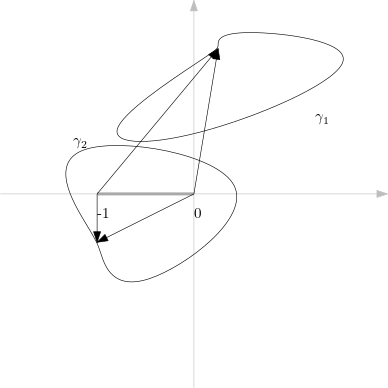
\includegraphics[scale=0.5]{Ex1.png}
		\label{fig:17.1}
\end{figure}
На кривых вида $\gamma_1$ (не опоясывающих разрез) приращение обоих аргументов
равно нулю (а значит, и суммарное), а на кривых вида $\gamma_2$ приращение
аргумента составит $8 \pi$. Оба случая удовлетворяют условию существования
регулярных ветвей.
\\
Докажем строго. Пусть $\os{\circ}{\gamma} = z(t)$, $t \in [0;1]$, $z(0) = z(1) =
z_0 \in \gamma$, $z(t, \alpha) = z(t) - \alpha$, $\alpha \in [-1;0]$. $\forall
(t, \alpha) \ z(t, \alpha) \neq 0$, $\forall \alpha \ z(1, \alpha) = z(0,
\alpha) = z_0 - \alpha$. Значит, по теореме $3$ $\S 14$ $I(\alpha) =
\Delta_{[0;1]}\argt z(t, \alpha) = const$, т.~е.
\begin{align*}
  & \Delta_{[0;1]} \argt z(t) = \Delta_{[0;1]} \argt(z(t) + 1) = \Delta_{\os{\circ}{\gamma}}z = \Delta_{\os{\circ}{\gamma}}(z+1) = 2 \pi k(\os{\circ}{\gamma})
\end{align*}
\begin{align*}
  & \Delta_{\ogamma} \argt f(z) = 4 \Delta_{\ogamma} \argt z = 8 \pi
\end{align*}
Желаемое условие выполняется.
\\
Значит,
\begin{align*}
  & g_1(z) = g_1(2) \sqrt[4]{\frac{\left| z^3(z+1) \right|}{24}} \exp \left( \frac{i}{4}\left( \Delta_{\gamma{2z}}\argt f(z) \right) \right)
\end{align*}
\begin{align*}
  & g_1(i) = g_1(2) \sqrt[4]{\frac{\left| i^3(i+1) \right|}{24}} \exp \left( \frac{i}{4}\left( \Delta_{\gamma_{2,i}}\argt f(z) \right) \right) = 2^{\frac{1}{8}}i\exp \left( \frac{i}{4} \left( 3\Delta_{\gamma_{2,i}}\argt z + \Delta_{\gamma_{2,i}} \argt (z+1) \right) \right) = \\
  & = 2^{\frac{1}{8}}i\exp \left( \frac{i}{4} \left( 3\frac{\pi}{2} + \frac{\pi}{4} \right) \right) = 2^{\frac{1}{8}}i\exp \left( \frac{7i\pi}{16} \right) =  2^{\frac{1}{8}}e^{\frac{15i\pi}{16}}
\end{align*}
\begin{align*}
  & g_1'(z) = \frac{4z^3+3z^2}{4g_1^3(z)}
\end{align*}
\begin{align*}
  & g_1'(i) = \frac{-4i -3}{4\cdot 2^{\frac{3}{8}}e^{\frac{45i\pi}{16}}} = -(4i+3)2^{-\frac{19}{8}}e^{-\frac{13i\pi}{16}}
\end{align*}
\Example
\begin{align*}
  & \Ln (1-z^2), \ G = \CC \setminus (-\infty; 1]
\end{align*}
Если ветвь существует, то
\begin{align*}
  & \Img h\left( \frac{i}{5} \right) = 0
\end{align*}
При этих условиях найти разложение $h$ в ряд Тейлора по степеням $(z+i)$,
область, где $h(z) = S(z)$~--- сумма своего ряда Тейлора, его радиус сходимости
$R$ и $S\left( \dst \frac{i}{5} \right)$.
\nonum
$G$ односвязна. Заметим: $f(z) = 1-z^2 \neq 0$ в $G$.
\\
$\forall \gamma \subseteq G$ рассмотрим $\Delta_{\gamma}\argt f(z)$.
\begin{align*}
  & h(z) = \ln \left| z \right| + i \Img h(z)
\end{align*}
\begin{align*}
  & h\left( \frac{i}{5} \right) = \ln \frac{26}{25}
\end{align*}
\begin{figure}[h!]
		\centering
		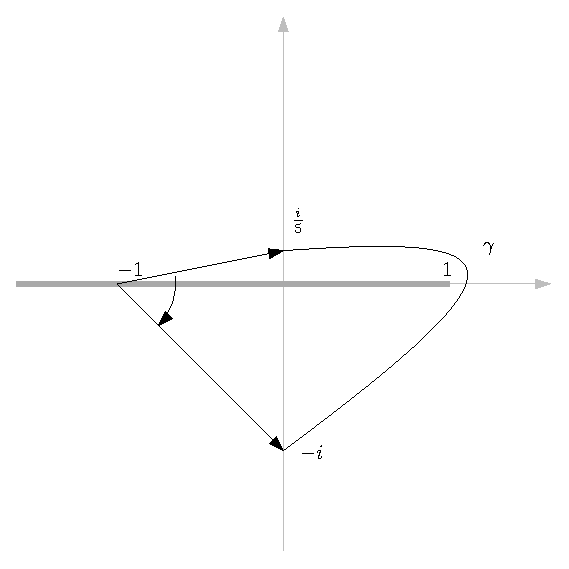
\includegraphics[scale=0.75]{Ex1.eps}
		\label{fig:17.2}
\end{figure}
\begin{align*}
  & h(-i) = \ln \frac{26}{25} + \ln \left| \frac{2}{\frac{26}{25}} \right|+ i\left( \Delta_{\gamma_{\frac{i}{5}, -i}}\argt (z+1) + \Delta_{\gamma_{\frac{i}{5}, -i}}\argt (z-1) + \Delta_{\gamma_{\frac{i}{5}, -i}}\argt (-1) \right) = \ln 2 - 2 i \pi
\end{align*}
Положим $\zeta = z+i$, $h(z) = h(\zeta - i) = \tilde{h}(\zeta)$. Тогда
$\tilde{h}(0) = h(-i) = \ln 2 - 2 i \pi$. Хотим разложить это в ряд.
\begin{align*}
  & \tilde{h}(\zeta) \in \Ln (1-(\zeta - i)^2) = \Ln(2+2i\zeta - \zeta^2) = \Ln \left(2\left( 1 - \frac{\zeta}{1-i} \right)\left( 1 - \frac{\zeta}{1+i} \right) \right) = \Ln 2 + \\
  & \Ln \left( 1 - \frac{\zeta}{1-i} \right) + \Ln \left( 1 - \frac{\zeta}{1+i} \right)
\end{align*}
Из теоремы об обратной функции
\begin{align*}
  & h^*_k(z) \in \Ln (1+z), \ \left| z \right| < 1 \Rightarrow h^*_k(z) = 2 i \pi k + \sum_{n=1}^\infty \frac{(-1)^{n+1}}{n} z^n, \ \left| z \right| < 1
\end{align*}
Рассмотрим
\begin{align*}
  & h_+(\zeta) \in \Ln \left( 1 - \frac{\zeta}{1+i} \right), \ \left| \zeta \right| < \sqrt{2}, \ h_+(0) = 0 \Rightarrow h_+(\zeta) = - \sum_{n=1}^\infty \frac{\zeta^n}{n(1+i)^n}, \ \left| \zeta \right| < \sqrt{2}
\end{align*}
\begin{align*}
  & h_-(\zeta) \in \Ln \left( 1 - \frac{\zeta}{1-i} \right), \ \left| \zeta \right| < \sqrt{2}, \ h_-(0) = 0 \Rightarrow h_-(\zeta) = - \sum_{n=1}^\infty \frac{\zeta^n}{n(1-i)^n}, \ \left| \zeta \right| < \sqrt{2}
\end{align*}
Заметим, что $\sqrt{2}$~--- максимальный радиус, т.~к. выходим на особую точку.
Видим:
\begin{align*}
  & \tilde{h}(\zeta) - h_+(\zeta) - h_-(\zeta) = \ln 2 + 2 i \pi k(\zeta)
\end{align*}
В правой части функция непрерывная, в левой ступенчатая, значит, $k = const$.
Найдем ее:
\begin{align*}
  &  \tilde{h}(0) - h_+(0) - h_-(0) = \ln 2 + 2 i \pi k = \ln 2 - 2 i \pi
\end{align*}
Значит, $k = -1$.
\\
Значит,
\begin{align*}
  & \tilde{h}(\zeta) = - \sum_{n=1}^\infty \frac{\zeta^n}{n(1+i)^n} - \sum_{n=1}^\infty \frac{\zeta^n}{n(1-i)^n} + \ln 2 - 2 i \pi
\end{align*}
\begin{align*}
  & h(z) = - \sum_{n=1}^\infty \frac{1}{n}\left( \frac{1}{(1+i)^n}+ \frac{1}{(1-i)^n}\right)(z-i)^n + \ln 2 - 2 i \pi, \ \left| z-i \right|< \sqrt{2}
\end{align*}
Видим, что $S(z)$ регулярна на $\left| z-i \right|< \sqrt{2}$; $S(z)$ и $h(z)$
есть регулярные ветви логарифма. Но также можем заметить, что часть разреза
лежит внутри круга сходимости. Тогда
\begin{align*}
  & \forall x \in (-1;1) \ h(x + i0) = h(x-i0) + i\Delta_{x+i0, x-i0}\argt h(z) = h(x-i0) + 2 i \pi \neq h(x-i0)
\end{align*}
Значит, внутри круга при положительной мнимой части $h(z) = S(z) + 2 i \pi$, а
при отрицательной мнимой части $h(z) = S(z)$.
\\
Значит,
\begin{align*}
  & S\left( \frac{i}{5} \right) = \ln \frac{25}{26} - 2 i \pi
\end{align*}
\begin{align*}
  & S'\left( \frac{i}{5} \right) = \left. \frac{-2z}{(1-z^2)} \right|_{z=\frac{i}{5}} = \frac{-2i\cdot 25}{5\cdot 26} = -\frac{5i}{13}
\end{align*}
\Def
Пусть $a, b \in \CC$, $a \neq 0$. Тогда
\begin{equation}\label{(17.1)}
    \left\{ a^b \right\} = \exp\left( b \Ln a\right)
\end{equation}
\Exse
Если $b = n$ или $b = \dst \frac{1}{n}$, $n\in \NN$, то \eqref{(17.1)} описывает
$a^n$ или $\left\{ \sqrt[n]{a} \right\}$ соответственно.
\Example
Разложить в ряд Тейлора регулярные ветви функции
\begin{align*}
  & \left\{ (1+z)^b \right\}, \ \left| z \right|<1
\end{align*}
\nonum
По определению,
\begin{align*}
  & (1+z)^b = \exp \left( b \Ln (1+z) \right)
\end{align*}
В силу существования регулярных ветвей у логарифма в этом круге ($h_k(0) = 2 i
\pi k$, $h_k$~--- регулярные ветви), то есть и регулярные ветви данной функции
будут существовать и иметь вид $w_k(z) = \exp \left( b h_k(z) \right)$.
\Exse
Доказать, что любая регулярная ветвь этой функции имеет такой вид.
\\
Вычислим производные $w_k$.
\begin{align*}
  & w_k(0) = e^{2bi\pi k}
\end{align*}
\begin{align*}
  & w_k'(z) = w_k(z) \frac{b}{1+z} \Rightarrow w_k'(0) = be^{2bi\pi k}
\end{align*}
\begin{align*}
  & w_k''(z) = w_k(z) \frac{b(b-1)}{(1+z)^2} \Rightarrow w_k''(0) = b(b-1)e^{2bi\pi k}
\end{align*}
\begin{align*}
  & w_k^{(n)}(z) = w_k(z) \frac{b(b-1)\dots(b-n+1)}{(1+z)^n} \Rightarrow w_k^{(n)}(0) = b(b-1)\dots(b-n+1)e^{2bi\pi k}
\end{align*}
\begin{align*}
  & w_k(z) = w_k(0)\sum_{n=0}^\infty C_b^nz^n
\end{align*}
\Example
Разложить в ряд Тейлора функцию
\begin{align*}
  & g \in \left\{ \sqrt[3]{1-z^2} \right\}, \ B_1(0), \ g(0) = \exp \left( \frac{2 i \pi}{3} \right)
\end{align*}
\nonum
По аналогии с предыдущим примером,
\begin{align*}
  & g(z) = \exp \left( \frac{2 i \pi}{3}\sum_{n=1}^\infty C_{\frac{1}{3}}^n(-1)^n z^{2n} \right)
\end{align*}
\Example
Разложить в $\os{\circ}{B}_1(\infty)$ в ряд Лорана регулярные ветви функции
\begin{align*}
  & \sets{\sqrt[4]{z^3(z+1)}}
\end{align*}
\nonum
\begin{align*}
  & \os{\circ}{B}_1(\infty) = \left\{ z \mid \left| z \right| > 1\right\}\subseteq \CC \setminus [-1;1]
\end{align*}
По аналогии с примером $1$
\begin{align*}
  & g_k(z) = \sqrt[4]{24}\exp \left( \frac{i\pi k}{2} \right)
\end{align*}
При $x > 2$, $x \in \RR$
\begin{align*}
  & g_0(x) = \sqrt[4]{x^3(x+1)} = x \sqrt[4]{1+\frac{1}{x}} = x \sum_{n=1}^\infty C_{\frac{1}{4}}^n\left( \frac{1}{x} \right)^n = S(x)
\end{align*}
\begin{align*}
  & \forall x \in \RR \cap (2; \infty) \ g_0(x) = S(x)
\end{align*}
Обе функции $S(z)$ и $g_0(z)$ регулярны, и по теореме единственности $g_0(z) =
S(z)$, а значит, искомый ряд Лорана будет иметь вид
\begin{align*}
  & z \sum_{n=1}^\infty C_{\frac{1}{4}}^n\left( \frac{1}{z} \right)^n
\end{align*}

    \begin{flushright}
    \textit{Лекция 14 (от 20.10)}
\end{flushright}
\section{$\S 18.$ Вычисление интегралов от регулярных ветвей.}
\Example
Вычислить при помощи теории вычетов интеграл
\begin{align*}
  & I = \int_0^2 \frac{\sqrt[4]{x^3(2-x)}}{(1+x)^2} dx
\end{align*}
\nonum
$g(z) = \sqrt[4]{z^3(2-z)}$ дает многозначную функцию. Отыщем регулярные ветви;
рассмотрим область, где ветви существуют. Функция $f(z) = z^3(2-z)$ должна быть
в области регулярной и не равной нулю.
\\
Рассмотрим $\CC \setminus [0;2]$. В такой области этот корень имеет регулярную
ветвь.
\\
Отыщем ветвь, что нам нужна. Построим ее так, чтобы $g(1+i0) = 1$; тогда
$\forall x \in [0;2] \ g(x+i0) = \sqrt[4]{x^3(2-x)}$. В этом случае
\begin{align*}
  & g(x-i0) = g(1+i0)\sqrt[4]{\frac{\left| g(x-i0) \right|}{\left| g(1+i0) \right|}}\exp\left( \frac{i}{4}\left( 3\Delta_{\gamma_{1+i0,x}}\argt z + \Delta_{\gamma_{1+i0,x}}\argt (2-z) \right) \right) = \\
  & = \sqrt[4]{\frac{\left| g(x-i0) \right|}{\left| g(1+i0) \right|}}\exp\left( \frac{-i\pi}{2}\right)
\end{align*}
\begin{figure}[h!]
		\centering
		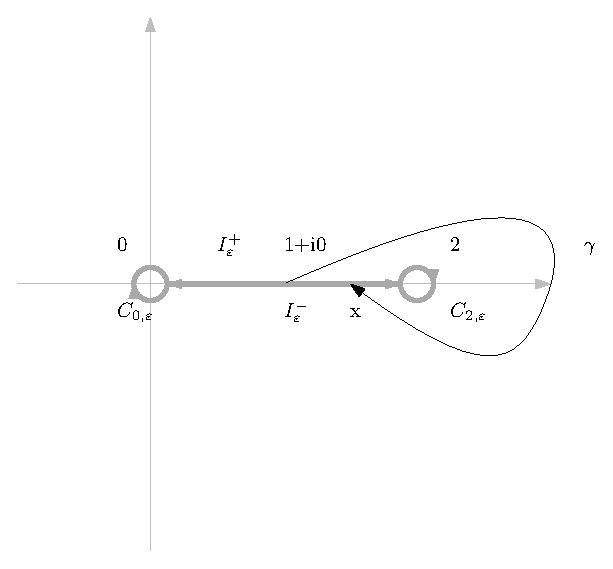
\includegraphics[scale=0.75]{Par18.eps}
		\label{fig:18.1}
\end{figure}
Рассмотрим
\begin{align*}
  & \gamma_\varepsilon = I_\varepsilon^+\cup C_{2, \varepsilon} \cup I_\varepsilon^-\cup C_{0, \varepsilon}
\end{align*}
и
\begin{align*}
  & F(z) = \frac{\sqrt[4]{z^3(2-z)}}{(1+z)^2} = \frac{g(z)}{(1+z)^2}
\end{align*}
и вычислим
\begin{align*}
  & I_\varepsilon = \int_{\gamma_\varepsilon}F(z) dz = 2 i \pi \left( \us{-1}{\res} F(z) + \us{\infty}{\res} F(z) \right)
\end{align*}
Видим, что $-1$~--- полюс $2$ порядка, а $\infty$~--- УОТ.
\begin{align*}
  & \us{-1}{\res} F(z) = \lim_{z \to -1}((z+1)^2F(z))' = \lim_{z \to -1}g'(z) = g'(-1) = \left. \frac{f'(z)}{4g^3(z)}\right|_{z = -1} = \frac{-4(-1)^3+6(-1)^2}{4\left( \sqrt[4]{3}\exp\left( \frac{3i\pi}{4} \right)\right)^3} = \\
  & = \frac{5}{2\sqrt[4]{27}}\exp\left( \frac{-i\pi}{4} \right)
\end{align*}
Рассмотрим $x \in (2; \infty)$; тогда
\begin{align*}
  & g(x) = \sqrt[4]{x^3(2-x)}\exp\left( \frac{-i\pi}{4} \right) = x\sqrt[4]{1-\frac{2}{x}}\exp \left( \frac{-i\pi}{4} \right) = x\exp\left( \frac{-i\pi}{4} \right)\sum_{n=0}^\infty C_{\frac{1}{4}}^n\left( -\frac{2}{x} \right)^n
\end{align*}
Две регулярные функции ($g(x)$ и сумма) совпадают на $(2; \infty)$, а значит, по
теореме единственности
\begin{align*}
  & g(z) = z\exp\left( \frac{-i\pi}{4} \right)\sum_{n=0}^\infty C_{\frac{1}{4}}^n\left( -\frac{2}{z} \right)^n, \ \left| z \right|> 2
\end{align*}
\begin{align*}
  & F(z) = \frac{z}{(z+1)^2}h(z), \ h(z) = \exp\left( \frac{-i\pi}{4} \right)\sum_{n=0}^\infty C_{\frac{1}{4}}^n\left( -\frac{2}{z} \right)^n
\end{align*}
Заметим, что
\begin{align*}
  & \frac{z}{(1+z)^2} = \frac{1}{z(1+\frac{1}{z})^2} = \frac{1}{z} \left( 1-\frac{2}{z} +\frac{3}{z^2} + \dots \right)
\end{align*}
При перемножении двух рядов получим
\begin{align*}
  & \us{\infty}{\res}F(z) = -\exp\left( \frac{-i\pi}{4} \right)
\end{align*}
и интеграл
\begin{align*}
  & I_\varepsilon = 2 i \pi \left( \frac{5}{2\sqrt[4]{27}} - 1 \right)\exp\left( \frac{-i\pi}{4} \right)
\end{align*}
не зависит от $\varepsilon$. Заметим, что
\begin{align*}
  & I_\varepsilon = \int_{I_\varepsilon^+}F(z) + \int_{C_{2, \varepsilon}}F(z) + \int_{I_\varepsilon^-}F(z) + \int_{C_{0, \varepsilon}}F(z)
\end{align*}
Причем
\begin{align*}
  & \int_{I_\varepsilon^+}F(z) = \int_{\varepsilon}^{2-\varepsilon}\frac{\sqrt[4]{x^3(2-x)}}{(x+1)^2}dx
\end{align*}
\begin{align*}
  & \int_{I_\varepsilon^-}F(z) = \int_{2-\varepsilon}^{\varepsilon}\frac{g(x-i0)}{(x+1)^2}dx = -\int_{\varepsilon}^{2-\varepsilon}\frac{\sqrt[4]{x^3(2-x)}\exp\left( \frac{3i\pi}{2} \right)}{(x+1)^2}dx = -\exp\left( \frac{3i\pi}{2}\right) \int_{I_\varepsilon^+}F(z)
\end{align*}
Учтя $z = \varepsilon e^{i \varphi}$,
\begin{align*}
  & \left|  \int_{C_{0, \varepsilon}}F(z) \right| \leq \int_{0}^{2 \pi}\frac{\varepsilon\sqrt[4]{\varepsilon^3(2+\varepsilon)}}{(1-\varepsilon)^2}d\varphi \leq A\varepsilon^{\frac{7}{3}} \us{\varepsilon \to 0}{\to} 0
\end{align*}
Учтя $z = 2 + \varepsilon e^{i \varphi}$,
\begin{align*}
  & \left|  \int_{C_{2, \varepsilon}}F(z) \right| \leq \int_{0}^{2 \pi}\frac{\varepsilon\sqrt[4]{(2+\varepsilon)^3\varepsilon}}{(3-\varepsilon)^2}d\varphi \leq B\varepsilon^{\frac{4}{3}} \us{\varepsilon \to 0}{\to} 0
\end{align*}
Значит,
\begin{align*}
  & 2 i \pi \left( \frac{5}{2\sqrt[4]{27}} - 1 \right)\exp\left( \frac{-i\pi}{4} \right) = I_\varepsilon \us{\varepsilon \to 0}{\to} \int_{I_\varepsilon^+}F(z) + \int_{I_\varepsilon^-}F(z) = \left( 1 -\exp\left( \frac{3i\pi}{2}\right) \right) \int_{I_\varepsilon^+}F(z) \us{\varepsilon \to 0}{\to} \\
  & \us{\varepsilon \to 0}{\to} \left( 1 -\exp\left( \frac{3i\pi}{2}\right) \right) I
\end{align*}
Значит,
\begin{align*}
  & I = \frac{2 i \pi \left( \dst \frac{5}{2\sqrt[4]{27}} - 1 \right)\exp\left( \dst\frac{-i\pi}{4} \right)}{\left( 1 -\exp\left( \dst \frac{3i\pi}{2}\right) \right)}= \pi \sqrt{2}\left( \dst \frac{5}{2\sqrt[4]{27}} - 1 \right)
\end{align*}
\section{$\S 19.$ Целые и мероморфные функции.}
\Def
Функция $f$ называется \textbf{целой}, если она регулярна на $\CC$.
\\
Можем представить такую функцию в виде
\begin{equation}\label{(19.1)}
    \forall z \in \CC \ f(z) = \sum_{n=0}^\infty c_nz^n, \ c_n = \frac{1}{2i\pi}\int_{\gamma_r}\frac{f(\zeta)}{\zeta^{n+1}} d \zeta
\end{equation}
\theorem
Пусть $f:G \mapsto \CC$ целая, $\exists A > 0, \ R > 0, \ m \in \NN_0$ такие,
что $\forall z: \left| z \right| > R \hookrightarrow \left| f(z) \right| \leq
A\left| z \right|^m$. Тогда $f(z)$~--- многочлен степени $\leq m$.
\pr
Воспользуемся оценкой $c_n$.
\begin{align*}
  & \forall r > R \ \left|c_n \right| \leq \frac{1}{2\pi}\int_{\left| \zeta \right| = r} \frac{\left| f(\zeta) \right|}{\left| \zeta \right|^{n+1}}\left| d\zeta \right|\leq \frac{1}{2\pi}\frac{Ar^m}{r^{n+1}}r\cdot 2 \pi = Ar^{m-n}
\end{align*}
Значит, $\forall n > m \ c_n = 0$.
\corollary (теорема Лиувилля)
Если $f$ целая, $\exists R > 0, \ A > 0$: $\left| f(z) \right|< A$ при $\left| z
\right| > R$, то $f \equiv const$.
\theorem (Основная теорема алгебры)
Всякий многочлен $P_n(z) = z^n + C_{n-1}z^{n-1}+\dots+c_0$ имеет в $\CC$ хотя бы
один корень.
\pr
предположим, $\forall z \in \CC \ P_n(z) \neq 0$. Тогда $\varphi(z) = \dst
\frac{1}{P_n(z)}$ целая. Но, как легко видеть,
\begin{align*}
  & \lim_{z \to \infty}P_n(z) = \infty \Rightarrow \lim_{z \to \infty} \varphi(z) = 0 \Rightarrow \exists R > 0: \ \forall z: \ \left| z \right| > R \hookrightarrow \left| \varphi(z) \right| < 1
\end{align*}
Значит, по теореме Лиувилля $\varphi(z) = const$, тогда и $P_n(z) = const$.
Противоречие.
\\
Значит, можем заметить, что для целой функции $f$ единственная особая точка~---
это $\infty$.
\begin{itemize}
    \item $\infty$~--- УОТ, тогда $f = const$.
    \item $\infty$~--- полюс порядка $m$, тогда $f = P_m$.
    \item $\infty$~--- СОТ.
\end{itemize}
\Def
Целая функция, у которой $\infty$ есть СОТ, назвается \textbf{целой
  трансцендентной}.
\theorem (Сохоцкого)
Пусть $f$~--- целая трансцендентная функция, тогда
\begin{align*}
  & \forall A \in \CCC \ \exists z_n \to \infty: \ \lim_{n \to \infty}f(z_n) = A
\end{align*}
\pr
Рассмотрим два случая.
\begin{itemize}
    \item $A = \infty$
    \\
    $f$ неограничена в окрестности $\infty$ (т.~к. иначе она бы имела конечный
    предел), т.~е.
    \begin{align*}
      & \forall n \in \NN \ \exists z_n \in \CC: \left| f(z_n) \right|> n, \ \left| z_n \right| > n
    \end{align*}
    Итак, $\left\{ z_n \right\}$ и есть та самая последовательность.
    \item $A \in \CC$
    \\
    Пусть, от противного,
    \begin{align*}
      & \exists \delta_0 > 0, \ \varepsilon_0 > 0: \ \forall z: \ \left| z \right| \geq \delta_0 \ \left| f(z) - A \right| \geq \varepsilon_0
    \end{align*}
    Пусть $\varphi(z) = \dst \frac{1}{f(z) - A}$, $z \in B_{\delta_0}(\infty)$.
    На этом множестве
    \begin{align*}
      & \left| \varphi(z) \right| \leq \frac{1}{\varepsilon_0}
    \end{align*}
    Значит, эта функция на этом множестве регулярна и ограничена, а значит, для
    нее $\infty$~--- УОТ, т.~е.
    \begin{align*}
      & \exists \lim_{z \to \infty}\varphi(z) = B
    \end{align*}
    Значит, $\infty$~--- полюс либо УОТ для $f(z)$, противоречие.
\end{itemize}
\theorem (общая теорема Сохоцкого)
Пусть $f: \os{\circ}{B}_r(a) \mapsto \CC$ регулярна, $a$~--- СОТ $f$. Тогда
\begin{align*}
  & \forall A \in \CCC \ \exists z_n \to a, \ \lim_{n \to \infty} f(z_n) = A
\end{align*}
\Exse
доказать общую теорему Сохоцкого.
\theorem (Пикара)
Пусть $f$~--- целая трансцедентная функция, тогда $\forall a \in \CC$, за
исключением, быть может, одного, $\exists R > 0$: в $\os{\circ}{B}_R(\infty)$
существует бесконечное число решений уравнения $f(z) = A$, т.~е.
\begin{align*}
  & \exists z_n \to \infty: \ \forall n \in \NN \ f(z_n) = A
\end{align*}
\Example
$e^z = A$ имеет счетное число решений в любой окрестности бесконечности при $A
\neq 0$, но ни одного решения при $A = 0$.
\Exse
Пусть $f$~--- целая функция и
\begin{align*}
  & \exists A > 0, R > 0, \ m \in \NN_0: \ \forall z: \ \left| z \right| > R \ \left| f(z) \right| \geq A \left| z \right|^m
\end{align*}
Доказать, что $f$~--- многочлен степени $\leq m$.
\Def
Функция $f$ называется мероморфной, если $\forall R > 0$ в круге $B_R(0)$ она
регулярна за исключением, быть может, конечного числа полюсов.
\Example
\begin{align*}
  & f(z) = \frac{P_n(z)}{Q_m(z)}
\end{align*}
Конечное число полюсов на всей $\CC$.
\Example
\begin{align*}
  & f(z) = \ctg z
\end{align*}
Счетное число полюсов на $\CC$.
\Example
\begin{align*}
  & f(z) = \frac{z}{e^z-1}
\end{align*}
Счетное число полюсов на $\CC$.
    \begin{flushright}
    \textit{Лекция 15 (от 26.10)}
\end{flushright}
$f$ мероморфна~--- тогда существует $\left\{ z_k \right\}_{n=1}^{\infty}$~---
полюсы $m_k$ порядков.
\\
Тогда $\exists \os{\circ}{B}_{\delta_k}(z_k)$, где ряд Лорана
\begin{equation}\label{(19.2)}
    f(z) = \frac{c^k_{-m_k}}{(z-z_k)^{m_k}} + \dots + \frac{c^k_{-1}}{z-z_k} + c_0^k= c_1^k(z-z_k) + \dots
\end{equation}
а его главная часть
\begin{equation}\label{(19.3)}
    q_k(z) = \frac{c^k_{-m_k}}{(z-z_k)^{m_k}} + \dots + \frac{c^k_{-1}}{z-z_k}
\end{equation}
\theorem
Пусть $f$ мероморфна, $\infty$~--- УОТ или полюс этой функции. Тогда $f$
рациональна.
\pr
$\left\{ z_k \right\}$~--- полюсы $m_k$ порядка. В силу изолированности $\infty$
набор полюсов конечен; пусть $k \in \left\{ 1, \dots, l \right\}$.
\\
$\infty$~--- УОТ или полюс; главная часть ряда Лорана в окрестности $\infty$
будет иметь вид
\begin{align*}
  & q_0 = c_1z+\dots +c_nz^n
\end{align*}
Из \eqref{(19.3)} получим $q_k(z)$ для любого $k$.
\\
Тогда
\begin{equation}\label{(19.4)}
    r(z) = f(z) - \sum_{k=0}^lq_k(z)
\end{equation}
Заметим, что $\forall k$ $r(z)$ имеет в $z_k$ устранимую особую точку. Эта
функция, доопределенная по непрерывности, будет регулярной в $\CC$ и
ограниченной на бесконечности, а значит, по теореме Лиувилля $r(z) \equiv a_0$.
Тогда из \eqref{(19.4)} получим
\begin{align*}
  & f(z) = a_0 + \sum_{k=0}^lq_k(z)
\end{align*}
а значит, $f$ рациональна.
\Def
Совокупность замкнутых простых кусочно гладких кривых $\left\{ \Gamma_n
\right\}_{n=1}^\infty$ называется \textbf{правильной}, если
\begin{itemize}
    \item $\forall n \in \NN$ область $D_n$, ограниченная $\Gamma_n$, содержится
    в области $D_{n+1}$, ограниченной $\Gamma_{n+1}$, причем $0 \in D_1$;
    \item $d_n = \min \left\{ \left| z \right| : z \in \Gamma_n \right\}
    \Rightarrow \dst \lim_{n \to \infty}d_n = \infty$;
    \item $\exists A > 0: \ \forall n \in \NN \ l_n \leq Ad_n$, где $l_n  =
    l(\Gamma_n)$.
\end{itemize}
\example
Вложенные окружности, вложенные квадраты с центром в точке $0$.
\theorem (Коши)
Пусть $f$ мероморфна и существует правильная совокупность $\left\{ \Gamma_n
\right\}_{n=1}^\infty$, такая, что:
\begin{itemize}
    \item $\varepsilon_n = \max\left\{ \left| f(z) \right|: z \in \Gamma_n
    \right\}: \ \dst \lim_{n \to \infty}\varepsilon_n = 0$
    \item $\left\{ z_n \right\}$~--- полюса, пронумерованные так, что $\forall n
    \in \NN$ в $D_n$ содержится ровно $n$ первых полюсов, а на $\Gamma_n$ полюсов
    нет.
\end{itemize}
Тогда $f(z)$ может быть представлена в виде ряда элементарных дробей:
\begin{equation}\label{(19.5)}
    f(z) = \sum_{k=1}^\infty q_k(z)
\end{equation}
причем $q_k$ определяется из \eqref{(19.3)}, а ряд \eqref{(19.5)} сходится
равномерно $\forall R > 0$ в $B_R(0)$ (за исключением полюсов).
\pr
$\forall n \in \NN$ определим
\begin{equation}\label{(19.6)}
    S_n(z) = \sum_{k=1}^n q_k(z)
\end{equation}
\begin{equation}\label{(19.7)}
    r_n(z) = f(z) - S_n(z)
\end{equation}
Фиксируем $n$, доопределяем $r_n$ в $D_n$ по непрерывности. Тогда эта функция
будет регулярной в этой области и непрерывной на ее границе $\Gamma_n$, а
значит, и на замыкании. По интегральной формуле Коши $\forall z \in D_n$
\begin{align*}
  & r_n(z) = \frac{1}{2 i \pi}\int_{\Gamma_n}\frac{r_n(\zeta)}{\zeta - z}d\zeta = \frac{1}{2 i \pi}\int_{\Gamma_n}\frac{f(\zeta)}{\zeta - z}d\zeta - \frac{1}{2 i \pi}\int_{\Gamma_n}\frac{S_n(\zeta)}{\zeta - z}d\zeta
\end{align*}
У функции $F_n(\zeta) = \dst \frac{S_n(\zeta)}{\zeta - z}$ внутри $D_n$ все
соответствующие $z_k$~--- особые точки, а вне $D_n$~--- $\infty$.
\begin{align*}
  & -\frac{1}{2 i \pi}\int_{\Gamma_n}F_n(\zeta) d\zeta = \us{\infty}{\res}F_n(\zeta)
\end{align*}
\begin{align*}
  & F_n(\zeta) = \sum_{k=1}^n\sum_{l=1}^{m_k}\frac{c_{-l}^k}{(\zeta - z)(\zeta - z_k)^{l}}
\end{align*}
Т.~к. $l+1 > 1$, то вычет равен нулю. Значит,
\begin{equation}\label{(19.8)}
    r_n(z) = \frac{1}{2 i \pi}\int_{\Gamma_n}\frac{f(\zeta)}{\zeta - z}d\zeta
\end{equation}
Фиксируем $R>0$. Тогда, в силу $d_n \to \infty$, $\exists N: \ \forall n \geq N
\ d_n > 2R$, и тогда
\begin{align*}
  & \left| r_n \right| \leq \frac{1}{2\pi}\us{\zeta \in \Gamma_n}{\max}\left| \frac{f(\zeta)}{\zeta - z} \right| l_n = \frac{\varepsilon_n l_n}{2\pi (d_n - R)} \leq \frac{\varepsilon_n}{\pi}A = \frac{A}{\pi}\varepsilon_n
\end{align*}
Значит, в $B_R(0)$ $r_n \rightrightarrows 0$. Соответственно, $S_n
\rightrightarrows f(z)$ в $B_R(0) \setminus \left( \dst
    \bigcup_{k=1}^{\infty}\left\{ z_k \right\} \right)$.
\Note
Пусть в тереме $7$ условие $\varepsilon_n \to 0$ заменено на $\exists B > 0, \ m
\in \NN: \ \varepsilon_n \leq Bd_n^m$. Тогда все условия теоремы $7$ выполняются
для функции $\dst \frac{f(z)}{z^{m+1}}$.
\pr (заметка)
В случае, если $0$ не является особой точкой, нужно добавить $\Gamma_0$~--- круг
малого радиуса с центром в нуле, лежащий в области $D_1$. Видим, что функция
$f(z)$, как и функция из замечания, разложима в этом случае в ряд элементарных
дробей.
\Example
Разложить в ряд элементарных дробей $w = \ctg z$.
\\
Знаем, что $z = \pi k, \ k \in \ZZ$~--- особые точки этой мероморфной функции.
Построим соответствующую правильную систему контуров.
\\
Положим $\tilde{z}_1 = 0$, $\tilde{z}_2 = \pi$, $\tilde{z}_3 = -\pi$,
$\tilde{z}_4 = 2 \pi$ и т.~д. Построим систему контуров:
% \begin{figure}[h!]
% 		\centering
% 		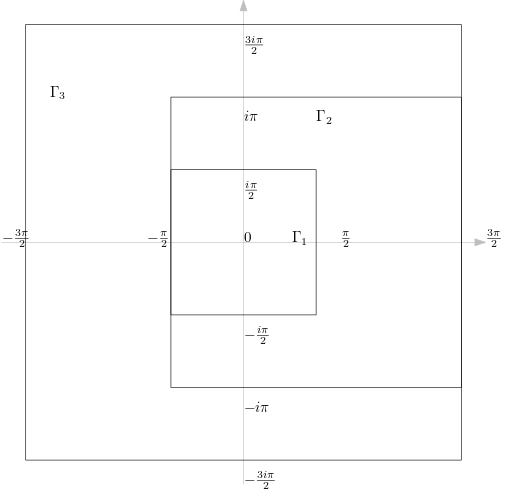
\includegraphics[scale=0.5]{Par20.png}
% 		\label{fig:19.1}
% \end{figure}
\begin{figure}[h!]
		\centering
		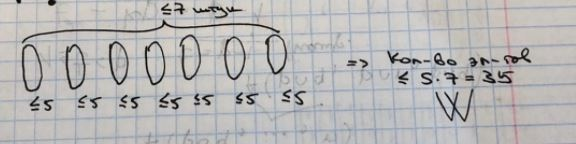
\includegraphics[scale=1]{20}
		\label{fig:19.2}
\end{figure}
Заметим, что $\Gamma_n$~--- квадраты, $l_n = 4\pi n$, $d_n \geq (n-1)\dst
\frac{\pi}{2}$, $\dst \frac{l_n}{d_n}\leq 16$. Значит, система контуров
правильная.
\\
Рассмотрим условия теоремы $7$. На вертикальных границах $\Gamma_n$ $z = \dst
\frac{\pi}{2} + \pi m + iy$. Тогда
\begin{align*}
  & \left| f(z) \right| = \frac{\left| \cos\left( \frac{\pi}{2}+\pi m + iy \right) \right|}{\left| \sin\left( \frac{\pi}{2}+\pi m + iy \right) \right|} = \frac{\left| \sin(iy) \right|}{\left| \cos(iy) \right|} = \frac{\left| e^{-y} - e^y \right|}{\left| e^{-y}+e^y \right|} \leq 1
\end{align*}
Видим, что функция ограничена на них. На горизонтальных границах $\Gamma_n$ $z =
x \pm i \dst \frac{\pi n}{2} = x+iy_n$. Тогда
\begin{align*}
  & \left| f(z) \right| = \frac{\left| e^{-y_n+ix}+e^{y_n-ix} \right|}{\left| e^{-y_n+ix}+e^{y_n-ix} \right|} \leq \frac{\left| e^{-y_n}+e^{y_n} \right|}{\left| e^{-y_n}+e^{y_n} \right|} \leq \frac{ 1+e^{-2\abs{y_n}}}{ 1-e^{-2\abs{y_n}}} \leq 2
\end{align*}
Видим, что функция ограничена на них.
\\
По замечанию $1$ $\dst \frac{\ctg z}{z}$ удовлетворяет условиям теоремы $7$, а
значит, $z = 0$~--- полюс второго порядка, $z_k = \pi k$~--- полюса первого
порядка, и тогда
\begin{align*}
  & \frac{\ctg z}{z} = \frac{\cos z}{z \sin z} = \frac{1 - \dst \frac{z^2}{2!} +\dots}{z^2 - \dst \frac{z^4}{3!}+\dots} = \frac{1}{z^2} +c_0 + c_1z + \dots
\end{align*}
\begin{align*}
  & q_0(z) = \frac{1}{z^2}
\end{align*}
\begin{align*}
  & z_k = \pi k, \ k \neq 0
\end{align*}
Значит,
\begin{align*}
  &  q_k = \frac{\us{\pi k}{\res}\dst \frac{\ctg z}{z}}{z - \pi k} = \frac{1}{\pi k (z - \pi k)}
\end{align*}
\begin{align*}
  & \frac{\ctg z}{z} = \frac{1}{z^2} +\sum_{^{k=-\infty}_{k \neq 0}}^{+\infty}\frac{1}{\pi k (z-\pi k)}
\end{align*}
\begin{align*}
  & \ctg z = \frac{1}{z} +\sum_{^{k=-\infty}_{k \neq 0}}^{+\infty}\frac{z+\pi k -\pi k}{\pi k (z-\pi k)} = \frac{1}{z} +\sum_{^{k=-\infty}_{k \neq 0}}^{+\infty}\left( \frac{1}{\pi k} + \frac{1}{z-\pi k}\right) = \frac{1}{z} +\sum_{k=1}^{\infty}\left( \frac{1}{\pi k} + \frac{1}{z-\pi k} + \frac{1}{-\pi k} + \right. \\
  &\left. \frac{1}{z+\pi k}\right) = \frac{1}{z} +\sum_{k=1}^{\infty}\left( \frac{1}{z-\pi k} + \frac{1}{z+\pi k}\right)
\end{align*}
\section{$\S 20.$ Принцип аргумента. Теорема Руше.}
\theorem
Пусть $f: G \mapsto \CC$
Пусть $G$~--- односвязная облась в $\CC$, $\ogamma$~--- простая замкнута
положительно ориентированная кривая в этой области. Пусть $f: G \mapsto \CC$
регулярна в $G$ за исключением, быть может, полюсов $a_1, \dots, a_k, \dots$,
лежащих внутри $\ogamma$. Пусть на $\ogamma$ нет особых точек $f$. Тогда
справедливо:
\begin{equation}\label{(20.1)}
    \frac{1}{2 i \pi}\int_{\ogamma} \frac{f'(z)}{f(z)}dz = N - P
\end{equation}
где $N$~--- число нулей, $P$~--- полюсов с учетом их порядка (каждый ноль или
полюс считаем такое число раз, каков его порядок)).
\pr
Пусть $b_1, \dots, b_n$~--- нули $f$ внутри $\ogamma$. В силу компактности
ограниченной $\ogamma$ области вместе с кривой и того. что $f(z) \not \equiv 0$,
их конечное число.
\\
Рассмотрим любой нуль $b = b_k$ порядка $m$. Тогда
\begin{align*}
  & f(z) = (z-b)^mh(z), \ z \in B_\varepsilon(b), \ \forall z \in B_\varepsilon(b) \ h(z) \neq 0
\end{align*}
Тогда
\begin{align*}
  & \frac{f'(z)}{f(z)} = \frac{m(z-b)^{m-1}h(z)+(z-b)^mh'(z)}{(z-b)^mh(z)} = \frac{m}{z-b} + \frac{h'(z)}{h(z)}
\end{align*}
и, значит,
\begin{align*}
  & \us{b}{\res}\frac{f'(z)}{f(z)} = m
\end{align*}
Пусть $a_1, \dots, a_p$~--- полюса, их, аналогично, тоже конечное число.
\\
Рассмотрим произвольный полюс $a = a_k$ порядка $l$. Тогда
\begin{align*}
& f(z) = \frac{p(z)}{(z-a)^l}, z \in \os{\circ}{B}_\delta(a), \ \forall z \in \os{\circ}{B}_\delta
(a) \ p(z)\neq 0
\end{align*}
Тогда
\begin{align*}
  & \frac{f'(z)}{f(z)} = \frac{-l}{z-a} + \frac{p'(z)}{p(z)}
\end{align*}
\begin{align*}
  & \us{a}{\res}\frac{f'(z)}{f(z)} = -l
\end{align*}
Отсюда по теореме Коши имеем \eqref{(20.1)}
\corollary (принцип аргумента)
В условии теорем $20.1$
\begin{equation}\label{(20.2)}
  \frac{1}{2\pi} \Delta_{\ogamma}\argt f(z) = N - P
\end{equation}
\pr
Пусть $\ogamma: z = z(t)$, $z(0) = z(1)$, $\ogamma$~--- гладкая замкнутая кривая.
\\
Пусть $\os{\circ}{\Gamma} = f(\ogamma)$, $0 \not \in \os{\circ}{\Gamma}$, $w =
f(z(t))$, $t \in [0;1]$.
\\
Тогда
\begin{align*}
  & \Real \int_{\os{\circ}{\Gamma}}\frac{dw}{w} = \Real \int_{\os{\circ}{\gamma}}\frac{f'(z)}{f(z)}dz = \ln\left| w \right| \Big|_{f(z(1))}^{f(z(0))} = 0
\end{align*}
\begin{align*}
  & \Img \int_{\os{\circ}{\Gamma}}\frac{dw}{w} = \Img \int_{\os{\circ}{\gamma}}\frac{f'(z)}{f(z)}dz = \Delta_{\ogamma}\argt f(z)
\end{align*}
\begin{align*}
  & \int_{\os{\circ}{\gamma}}\frac{f'(z)}{f(z)}dz = i\Delta_{\ogamma}\argt f(z)
\end{align*}
Тогда из \eqref{(20.1)} очевидно следует \eqref{(20.2)}.
    \begin{flushright}
    \textit{Лекция 16 (от 27.10)}
\end{flushright}
\theorem (Руше)
Пусть $G$~--- односвязная область, $\ogamma$~--- замкнутая положительно
ориентированная кусочно гладкая кривая в этой области. Пусть $f,g: G \mapsto
\CC$ регулярны, и
\begin{equation}\label{(20.3)}
    \forall z \in \ogamma \ \left| f(z) \right| > \left| g(z) \right|
\end{equation}
Тогда $f(z)$ и $h(z) = f(z)+g(z)$ имеют внутри $\ogamma$ одинаковое число нулей
с учетом их порядка.
\pr
\begin{align*}
  & \forall z \in \ogamma \ \left| f(z) \right| > \left| g(z) \right| \Rightarrow \forall z \in \ogamma \ f(z) \neq 0
\end{align*}
\begin{align*}
  & \forall z \in \ogamma \ \left| h(z) \right|\geq \left| f(z) \right| - \left| g(z) \right| > 0 \Rightarrow \forall z \in \ogamma h(z) \neq 0
\end{align*}
\begin{align*}
  & \Delta_{\ogamma}\argt h(z) = \Delta_{\ogamma} \argt \left( f(z)\left( 1+\frac{g(z)}{f(z)} \right) \right) = \Delta_{\ogamma}\argt f(z) +\Delta_{\ogamma}\argt \left( 1+\frac{g(z)}{f(z)} \right)
\end{align*}
\begin{align*}
  & \ogamma: w = 1 + \frac{g(z)}{f(z)} \Rightarrow \left| w-1 \right| = \left| \frac{g(z)}{f(z)} \right| < 1
\end{align*}
Пусть $\Gamma = w(\ogamma) \subseteq B_1(1)$; $0 \not \in B_1(1)$ и эта область
односвязна, значит, по теореме $3$ $\S 14$
\begin{align*}
  & \Delta_{\ogamma}\argt \left( 1+\frac{g(z)}{f(z)} \right) = 0
\end{align*}
и тогда
\begin{align*}
  & N_h = \frac{1}{2\pi}\Delta_{\ogamma}\argt h(z) = \frac{1}{2\pi}\Delta_{\ogamma}\argt f(z) = N_f
\end{align*}
\theorem (Гаусса)
Многочлен
\begin{align*}
  & P_n(z) = c_0+zc_1+z^2c_2+\dots+z^nc_n
\end{align*}
имеет в $\CC$ ровно $n$ корней с учетом их порядка.
\pr
Рассмотрим $f(z) = c_nz^n$, $g(z) = P_n(z) - f(z)$. Как известно,
\begin{align*}
  & \left| \frac{g(z)}{f(z)} \right| \us{z \to \infty}{\to} 0 \Rightarrow \exists R_0 > 0: \ \forall R \geq R_0 \ \forall z \in \gamma_R \ \left| f(z) \right| > \left| g(z) \right|
\end{align*}
Значит, по теореме Руше функция $P_n(z)$ имеет столько же нулей, сколько и $f(z)
= c_nz^n$, на $B_R(0)$, с учетом порядка, т.~е. ровно $n$ штук.
\Example
Функция Жуковского
\begin{align*}
  & w = \frac{1}{2}\left( z+\frac{1}{z} \right)
\end{align*}
У функции $\pm i$~--- нули, $0$~--- полюс первого порядка.
\\
Рассматривая $R>1$, получим
\begin{align*}
  & \Delta_{\gamma_R}\argt w(z) = 2 \pi (N-P) = 2\pi
\end{align*}
\begin{align*}
  & \Delta_{\gamma_{\frac{1}{R}}}\argt w(z) = 2 \pi (N-P) = -2\pi
\end{align*}
\section{$\S 21.$ Геометрические принципы.}
\lemma (об открытости)
Пусть $f$ регулярна в $G$, $z_0 \in G$, $w_0 = f(z_0)$.
\\
Пусть при $n \geq 2$
\begin{equation}\label{(21.1)}
    f'(z_0) = \dots = f^{(n-1)}(z_0) = 0, \ f^{(n)}(z_0) \neq 0
\end{equation}
Тогда $\exists B_\delta(z_0)$ и $B_\varepsilon(w_0)$, такие, что $\forall w_1
\in B_{\varepsilon}(w_0)$ уравнение $f(z) = w_1$ имеет в круге $B_\delta(z_0)$
ровно $n$ решений.
\pr
Заметим, что $f(z) \neq const$, $f'(z) \neq const$. Тогда по теореме
единственности нули функции $f(z)-w_0$ и $f'(z)$ изолированы, поэтому
\begin{align*}
  & \exists \delta > 0: \ \forall z \in \ol{\os{\circ}B_\delta(z_0)}\setminus\{z_0\} \ f(z)-w_0 \neq 0, \ f'(z) \neq 0
\end{align*}
Пусть $\gamma = \left\{ z: \left| z-z_0 \right| = \delta \right\}$ положительно
ориентирована, и $\forall z \in \gamma \ f(z)\neq w_0$. Положим $0 < \varepsilon
= \inf \left\{ w_0 - f(z) \mid z \in \gamma \right\}$, $\Gamma = f(\gamma)$.
заметим, что $\Gamma$ замкнута и $w_0 \not \in \Gamma$.
\\
Тогда
\begin{align*}
& \forall w_1 \in \os{\circ}{B}_\varepsilon(w_0), \ \forall z \in \gamma \ \left| w_1-w_0 \right| < \varepsilon \leq \left| w_0 - f(z) \right|
\end{align*}
Пусть $F(z) = w_0 - f(z)$, $G(z) = w_1-w_0$. Тогда $H(z) = F(z)+G(z) =
w_1-f(z)$; значит, по теореме Руше (в силу $\left| F(z) \right|> \left| G(z)
\right|$) функции $w_0 - f(z)$ и $w_1-f(z)$ имеют одинаковое число нулей внутри
$\gamma$. 
\\
Заметим, что $f(z) = w_0$ имеет единственный нуль~--- $z_0$~--- порядка $n$.
Значит, с учетом порядка $f(z) = w_1$ имеет $n$ решений.
\\
Но 
\begin{align*}
& \forall z \in B_\delta(z_0) \ f'(z) = (f(z)-w_1)' \neq 0
\end{align*}
Значит, все нули будут иметь первый порядок, соответственно, их ровно $n$ штук.
\corollary
Пусть $f$ регулярна в $G \subseteq \CC$. Тогда $\forall z_0 \in G$ условие
$f'(z_0) \neq 0$ необходимо и достаточно для однолистности $f$ <<в малом>>~--- в
некоторой достаточно малой окрестности $z_0$, но не во всей $G$.
\Example
$w=e^z$ удовлетворяет условиям следствия, но не однолистна во всей комплексной
плоскости.
\theorem (принцип сохранения области)
Пусть $f$ регулярна в области $G$, причем $f(z) \neq const$. Тогда $f(G)$~---
также область.
\pr
Докажем открытость.
\begin{align*}
& \forall z_0 \in G \ w_0 = f(z_0) \in G^* = f(G)
\end{align*}
Поскольку $G$~--- область, 
\begin{align*}
& \exists \delta_1: \ B_{\delta_1}(z_0) \subseteq G
\end{align*}
и по лемме $21.1$
\begin{align*}
& \exists \delta \in (0; \delta_1], \ \exists \varepsilon > 0: \ \forall w_1 \in B_\varepsilon (w_0) \ \exists z_1 \in B_\delta(z_0): \ f(z_1) = w_1; \ f(B_\delta(z_0)) \supseteq B_\varepsilon(w_0)
\end{align*}
Значит, $B_\varepsilon(w_0)\subseteq G^*$, т.~е. $w_0$~--- внутренняя точка $G^*$.
\\
Докажем связность.
\begin{align*}
  & \forall w_1, w_2 \in G^* \ \exists z_1,z_2 \in G: \ \exists \gamma_{z_1z_2} \subseteq G, \ \Gamma_{w_1w_2} = f(\gamma_{z_1z_2}) \subseteq G^*
\end{align*}
\theorem (принцип максимума модуля регулярной функции)
Пусть $f: G \mapsto \CC$ регулярна в ограниченной области $G$, непрерывна на ее
замыкании и непостоянна. Тогда
\begin{align*}
  & \max_{z \in \ol{G}} \left| f(z) \right| = \max_{z \in \partial G} \left| f(z) \right|
\end{align*}
\pr
Путь, от противного,
\begin{align*}
  & \exists z_0 \in G: \ \left| f(z_0) \right| = \max_{z \in \ol{G}}\left| f(z) \right|
\end{align*}
Пусть $w_0 = f(z_0)$. По теореме $21.1$
\begin{align*}
  & \exists \varepsilon > 0, \ B_\varepsilon(w_0) \subseteq f(G) = G^*
\end{align*}
\begin{align*}
  & w_1 \in B_\varepsilon(w_0): \left| w_1 \right| > \left| w_0 \right|; \ w_1 = w_0\left( 1+\frac{\varepsilon}{2\left| w_0 \right|} \right)
\end{align*}
\begin{align*}
  & \exists z_1 \in G: \ f(z_1) = w_1; \ \left| f(z_1) \right| > \left| f(z_0) \right|
\end{align*}
Противоречие.
\corollary (принцип минимума модуля регулярной функции)
Пусть $f: G \mapsto \CC$ регулярна в ограниченной области $G$, непрерывна на ее
замыкании и непостоянна; $\forall z \in G \ f(z) \neq 0$. Тогда
\begin{align*}
  & \min_{z \in \ol{G}} \left| f(z) \right| = \min_{z \in \partial G} \left| f(z) \right|
\end{align*}
\Note
Для случая неограниченной $G$ вместо $\min$ и $\max$ используется $\inf$ и
$\sup$.
\lemma (Шварца)
Пусть $f: B_1(0) \mapsto \CC$ регулярна, $\forall z \in B_1(0) \ \left| f(z)
\right| \leq 1$, $f(0) = 0$. Тогда выполняется
\begin{equation}\label{(21.2)}
    \forall z \in B_1(0) \ \left| f(z) \right| \leq z
\end{equation}
Если в \eqref{(21.2)} достигается равенство при $z_0 \neq 0$, то
\begin{align*}
  & \exists \alpha \in \RR: \ \forall z \in \ol{B_1(0)} \ f(z) = e^{i\alpha}z
\end{align*}
\pr
$f(0) = 0$, а значит, существует регулярная в $B_1(0)$ функция $g(z)$: $f(z) =
zg(z)$. Функция $g(z) = \dst \frac{f(z)}{z}$, но при этом регулярна также и в
нуле.
\\
Рассмотрим произвольное $r \in (0;1)$ и $z: \ \left| z \right|<r$. По теореме
$2$
\begin{align*}
  & \left| g(z) \right| \leq \max \left\{ \left| \frac{f(\zeta)}{\zeta} \right| : \left| \zeta \right| =r \right\} \leq \frac{1}{r}
\end{align*}
Пусть $z_0 \in B_1(0)$; $\forall r \in (\left| z_0 \right|, 1)$ $\left| g(z_0)
\right| \leq \dst \frac{1}{r}$, а значит, $\left| g(z_0) \right|\leq 1$, и
$\forall z \in B_1(0) \ \left| f(z) \right|\leq \left| z \right|$.
\\
Пусть равенство в \eqref{(20.2)} достигается в некоторой точке $z_1$ (т.~е.
$\left| g(z) \right| = 1$). Поскольку точка лежит внутри области, то либо
возникает противоречие с принципом максимума, либо $g(z) = const = e^{i
  \alpha}$.
\theorem (принцип максимума и минимума гармонической функции)
Пусть $u: G \mapsto \CC$ гармоническая на $G \subseteq \RR^2$ и непостоянная,
непрерывная на $\ol{G}$. Тогда $\sup$ и $\inf$ функции $u$ на $G$ и $\ol{G}$
совпадают.
\pr
Допустим, $\exists z_0 = (x_0, y_0)\in G$, на которой $u$ достигает максимума.
Тогда $\exists \varepsilon > 0: \ B_\varepsilon(z_0)\subseteq G$; по теореме $2$
$\S 4$ сущствует регулярная $f$ в $B_\varepsilon(z_0)$ такая, что $\Real f(z) =
u(z)$.
\\
$w_0 = f(z_0)$; по теореме $21.1$ $f(B_\varepsilon(z_0))$~--- область, т.~е.
$\exists r > 0$: $B_r(w_0) \subseteq f(B_{\varepsilon}(z_0))$. Пусть $w_1 \in
B_r(w_0)$, $\Real w_1 > \Real w_0$.
\\
Значит,
\begin{align*}
  \exists z_1 \in B_\varepsilon(z_0): \ w_1 = f(z_1), \ \Real f(z_1) > \Real f(z_0) \Rightarrow u(z_1)>u(z_0)
\end{align*}
Противоречие.
\\
В силу $\inf u(z) = - \sup(-u(z))$, гармоничности $-u(z)$ и выполнимости
принципа максимума выполняется и принцип миминума.
\theorem (о среднем для гармонической функции)
Пусть $u: B_R(z) \mapsto \RR$ гармоническая и непрерывная на замыкании
этого круга, непостоянная. Тогда
\begin{equation}\label{(21.3)}
    u(a) = \frac{1}{2\pi}\int_0^{2\pi}u(a+Re^{i\varphi})d\varphi
\end{equation}
\pr
По теореме $2$ $\S 4$ существует $f: B_R(a) \mapsto \CC$~--- регулярная, причем
$\forall z \in B_R(a) \ \Real f(z) = u(z)$, $0<\rho < R$, $\gamma_\rho =
\left\{ z: \left| z-a \right| = \rho\right\}$.
\begin{align*}
  & f(a) = \frac{1}{2 i \pi}\int_{\gamma_\rho}\frac{f(\zeta)}{\zeta - a}d\zeta = \frac{1}{2i\pi}\int_0^{2\pi}\frac{f(a+\rho e^{i\varphi})}{\rho e^{i\varphi}} i \rho e^{i\varphi} d \varphi = \frac{1}{2\pi}\int_0^{2\pi}f(a+\rho e^{i\varphi})d \varphi
\end{align*}
\begin{align*}
  & \Real f(a) = u(a) = \frac{1}{2\pi}\int_0^{2\pi}\Real f(a+\rho e^{i\varphi})d \varphi = \frac{1}{2\pi}\int_0^{2\pi}u (a+\rho e^{i\varphi})d \varphi
\end{align*}
Устремляя $\rho \to R$, получаем \eqref{(21.3)}.

    \begin{flushright}
    \textit{Лекция 17 (от 02.11)}
\end{flushright}
\section{$\S 22.$ Конформные отображения в $\overline{\CC}$.}
\begin{center}
    \textbf{Геометрический смысл аргумента и модуля производной}
\end{center}
Рассмотрим $f: B_r(z_0) \mapsto \CC$, $f'(z_0) \neq 0$.
\\
Пусть $w = f(z)$, $w_0 = f(z_0)$, $w-w_0 = f'(z_0)(z-z_0) + o(z-z_0)$.
\\
Покоординатно:
\begin{align*}
  & f'(z_0) = u_x+iv_x, \ f=u+iv
\end{align*}
\begin{align*}
  & \left( \begin{matrix}
          \Delta u \\
          \Delta v
      \end{matrix} \right) = \left( \begin{matrix}
          u_x & -v_x \\
          v_x & u_x
      \end{matrix} \right)  \left( \begin{matrix}
          \Delta x \\
          \Delta y
      \end{matrix} \right) = K \left( \begin{matrix}
          \frac{u_x}{K} & \frac{-v_x}{K} \\
          \frac{v_x}{K} & \frac{u_x}{K}
      \end{matrix} \right) \left( \begin{matrix}
          \Delta x \\
          \Delta y
      \end{matrix} \right)
\end{align*}
\begin{align*}
  & K = \sqrt{u^2_x+v^2_x} = \left| f'(z_0) \right|
\end{align*}
Видим, что это ортогональное преобразование.
\\
\textbf{Свойство сохранения окружности в малом:}
\\
Рассмотрим $\gamma_r = \left\{ z: \left| z-z_0 \right| = r, \ 0 < r <
    r_0\right\}$. Пусть в области, ограниченной кривой, производная ненулевая.
\begin{align*}
  & \left| \Delta w \right| \approx \left| f'(z_0) \right|\cdot \left| \Delta z \right| \approx K r
\end{align*}
(получаем <<примерно окружность>>).
\\
\textbf{Свойство сохранения углов:}
\\
Рассмотрим теперь $\gamma_1, \gamma_2: \ z = z_k(t), \ t \in \left[ t_0 -\delta;
    t_0+\delta\right], \ z_k(t_0) = z_0$. Пусть при таких $t$ $z'_k\neq 0$, угол
между кривыми $\alpha$. Пусть $\gamma_1^* = f(\gamma_1)$, $\gamma_2^* =
f(\gamma_2)$. Тогда угол между $\gamma_1^*$ и $\gamma_2^*$ также равен $\alpha$.
\\
Действительно,
\begin{align*}
  & w'_k(t_0) = f'(z_0)z'_k(t_0)
\end{align*}
\begin{align*}
  & \Arg w'_k(t_0) = \argm f'(z_0) + \Arg z'_k(t_0)
\end{align*}
(изменение на одинаковый угол).
\begin{center}
    \textbf{Конформные отображения в $\CC$}
\end{center}
\Def
Функция $f: G \mapsto \CC$ называется \textbf{конформной в точке $z_0$}, если
$f= u+iv$, $u$ и $v$ дифференцируемы в $z_0$ и линейное отображение вида
\begin{equation}\label{(22.1)}
    \begin{cases}
        du = u_x(x_0,y_0)\Delta x + u_y(x_0,y_0) \Delta y \\
        dv = v_x(x_0,y_0)\Delta x + v_y(x_0,y_0) \Delta y
    \end{cases}
\end{equation}
является суперпозицией линейного растяжения и поворота относительно нуля.
\theorem
Функция $f$ конформна в $Z_0 \in \CC$ тогда и только тогда, когда она в этой
точке дифференцируема, а производная отлична от нуля.
\pr
~
\begin{itemize}
    \item $\Leftarrow$
    \\
    Следует из геометрического смысла и определения.
    \item $\Rightarrow$
    \\
    Пусть $f$ конформна в $z_0$. Тогда $\exists K > 0$, $\exists \theta \in
    [0;2\pi)$ такие, что из \eqref{(22.1)} получаем
    \begin{equation}\label{(22.2)}
        \left( \begin{matrix}
                \Delta u \\
                \Delta v
            \end{matrix} \right) = K \left( \begin{matrix}
                \cos \theta & \sin \theta \\
                -\sin \theta & \cos \theta
            \end{matrix} \right) \left( \begin{matrix}
                \Delta x \\
                \Delta y
            \end{matrix} \right)
    \end{equation}
    В силу дифференцируемости $u$ и $v$
    \begin{align*}
      & u_x = K \cos \theta, \ u_y = K \sin \theta, \ v_x = -K \sin \theta, \ u_y = K \cos \theta
    \end{align*}
    Выполняется УКР, значит, $\exists f'(z_0)$, $\left| f'(z_0) \right| = K >
    0$.
\end{itemize}
\Def
$f: G \mapsto \CC$ \textbf{конформна на области $G$}, если $f$ однолистна на $G$
и конформна в каждой ее точке.
\corollary
$f$ конформна в $G \subset \CC$ $\Leftrightarrow$ $f$ однолистна и регулярна в
$G$.
\begin{center}
    \textbf{Конформные отображения в $\CCC$}
\end{center}
\underline{\textbf{Свойства стереографической проекции}}
\begin{enumerate}
    \item Образы любых двух пересекающихся кривых на комплексной плоскости будут
    пересекаться на сфере Римана под тем же углом.
    \item $w = \frac{1}{z}: \CCC \mapsto \CCC$ соответствует при
    стереографической проекции отображению сферы Римана на себя путем поворота
    ее на $\pi$ относительно ее диаметра с концами в точках, являющихся образами
    $1$ и $-1$ на $\CC$.
\end{enumerate}
\Def
Пусть $f$ имеет УОТ в $\infty$. Тогда $f$ называется \textbf{конформной в
  $\infty$}, если $g(z) = f\left( \dst \frac{1}{z} \right)$, доопределенная по
непрерывности в нуле, конформна в нуле.
\Def
Пусть $a \in \CCC$~--- полюс или СОТ $f$. Тогда $f$ называется
\textbf{конформной в $a$}, если $\varphi(z) = \dst \frac{1}{f(z)}$,
доопределенная по непрерывности, конформна в этой точке.
\Exse
Доказать, что в определении $22.4$ допустим лишь полюс $1$ порядка.
\Def
Пусть $f: G \mapsto \CCC$. Тогда $f$ называется \textbf{конформной в области
  $G$}, если она однолистна на ней и конформна в каждой ее точке.
\prop
$f$ конформна в $G \subseteq \CCC$, если $f$ однолистна на ней и регулярна на
ней, за исключением, быть может, двух точек:
\begin{itemize}
    \item $\infty$, если $\infty \in G$ и является УОТ или полюсом $1$ порядка;
    \item $a \in G$, $a \neq \infty$~--- полюс $1$ порядка, если $\infty$~---
    УОТ или $\infty \not \in G$.
\end{itemize}
\section{$\S 23.$ Дробно-линейные функции.}
\Def
Функция
\begin{equation}\label{(23.1)}
    w = \frac{az+b}{cz+d}, \ a,b,c,d \in \CC, \ ad-cb \neq 0
\end{equation}
называется \textbf{дробно-линейной функцией (ДЛФ)} и задает
\textbf{дробно-линейное отображение (ДЛО).} Бывает:
\begin{equation}\label{(23.2)}
    \left[ \begin{matrix}
            c = 0 \Rightarrow w = az+b \Rightarrow w(\infty) = \infty \\
            c \neq 0 \Rightarrow w(\infty) = \dst \frac{a}{c}, \ w\left( -\dst \frac{d}{c} \right) = \infty
        \end{matrix} \right.
\end{equation}
ДЛФ \eqref{(23.1)}, \eqref{(23.2)} действует из $\CCC$ в $\CCC$.
\theorem
ДЛФ \eqref{(23.1)}, \eqref{(23.2)} конформно отображает $\CCC$ на $\CCC$.
\pr
~
\begin{enumerate}
    \item Проверим однолистность на $\CCC$.
    \\
    Из \eqref{(23.1)}
    \begin{equation}\label{(23.3)}
        z = \frac{dw-b}{cw-a}
    \end{equation}
    Видим, что $ad - cb \neq 0$, а значит, существует обратное ДЛО.
    \item Покажем конформность в каждой точке.
    \begin{itemize}
        \item $z_0 \neq - \dst \frac{d}{c}$, $z_0 \in \CC$. Тогда
        \begin{align*}
          & w'(z_0) = \frac{ad-cb}{(cz_0+d)^2} \neq 0
        \end{align*}
        что и хотим видеть.
        \item $z_0  = -\dst \frac{d}{c}$. Положим
        \begin{align*}
          & \varphi(z) = \frac{1}{f(z)} = \frac{cz+d}{az+b}
        \end{align*}
        и тогда
        \begin{align*}
          & \varphi'(z_0) = \frac{cb - ad}{\left( -a\dst \frac{d}{c} + b \right)^2} = \frac{c^2}{-ad + bc} \neq 0
        \end{align*}
        что и хотим видеть.
        \item $z_0 = \infty$. Положим
        \begin{align*}
          & g(z) = f\left( \frac{1}{z} \right) = \frac{a+bz}{c+dz}
        \end{align*}
        и тогда
        \begin{align*}
          & g'(z_0) = \frac{bc - ad}{c^2} \neq 0
        \end{align*}
        что и хотим видеть.
    \end{itemize}
\end{enumerate}
\Exse
Пусть $f: \CCC \mapsto \CCC$ конформно, тогда $f$~--- ДЛФ. Доказать это
утверждение.
\theorem
При ДЛО \eqref{(23.1)}, \eqref{(23.2)} образом окружности или прямой будет
окружность или прямая.
\pr
~
\begin{enumerate}
    \item Рассмотрим аффинное отображение $w = az+b$ ($c = 0$).
    \\
    Знаем из аналитической геометрии, что окружность переходит в окружность, а
    прямая~--- в прямую.
    \item Рассмотрим теперь $c \neq 0$.
    \\
    Представим отображение в виде
    \begin{align*}
      & w = \frac{az+b}{cz+d} = \frac{a}{c} + \frac{-ad+bc}{c}\cdot \frac{1}{cz+d}
    \end{align*}
    \begin{equation}\label{(23.4)}
        w = \alpha + \beta t, \ \alpha = \frac{a}{c}, \ \beta = \frac{-ad+bc}{c}, \ t = \frac{1}{\zeta}, \ \zeta = cz+d
    \end{equation}
    Видим, что $w(t)$ и $\zeta(z)$~--- аффинные, проверим выполнимость
    утверждения теоремы для $z = \dst \frac{1}{\zeta}$.
    \\
    Положим $\zeta = \xi + i \eta$. Уравнение
    \begin{align*}
      & A(\xi^2+\eta^2) + B\xi + C\eta + D = 0, \ 4AD < B^2+C^2
    \end{align*}
    задает невырожденную окружость при $A \neq 0$ и невырожденную прямую при $A =
    0$. Полагая $t = \dst \frac{1}{\zeta}$, учитывая $\xi^2 + \eta^2 =
    \zeta\bar{\zeta}$, $\xi = \dst \frac{\zeta + \bar{\zeta}}{2}$, $\eta = \dst
    \frac{\zeta - \bar{\zeta}}{2i}$, запишем уравнение в виде
    \begin{align*}
      & A\zeta\bar{\zeta} + \left( \frac{B}{2} + \frac{C}{2i}\right)\zeta + \left( \frac{B}{2} - \frac{C}{2i}\right)\bar{\zeta} + D = 0
    \end{align*}
    и отсюда получим
    \begin{align*}
      & A + \left( \frac{B}{2} + \frac{C}{2i}\right)\bar{t} + \left( \frac{B}{2} - \frac{C}{2i}\right)t + Dt\bar{t} = 0
    \end{align*}
    что задает окружность при $D \neq 0$ и прямую при $D = 0$. Суперпозиция
    преобразований, переводящих окружности и прямые в окружности и прямые,
    переводит окружности и прямые в окружности и прямые.
\end{enumerate}
\Note
Окружность или прямая $\gamma$ переходит при ДЛО в прямую, если нуль знаменателя
принадлежит $\gamma$, и в окружность иначе.
\\
Это называется \textbf{круговым свойством}.
\Def
Точки $M$ и $M^*$ называются \textbf{симметричными относительно окружности с
  центром в точке $A$ радиуса $R > 0$}, если они лежат на одном луче, исходящем
из точки $A$, и $\left| AM \right| \cdot \left| AM^* \right| = R^2$. На $\CCC$
$z$ и $z^*$ симметричны относительно окружности $\gamma_r$ с центром в точке
$a$, если
\begin{equation}\label{(23.5)}
    z^* - a = \frac{R^2}{\bar{z} - \bar{a}}
\end{equation}
Заметим, что при $z \to a$ $z^* \to \infty$, т.~е. $a$ и $\infty$ симметричны.
    \begin{flushright}
    \textit{Лекция 18 (от 03.11)}
\end{flushright}
\theorem
При ДЛО пара симметричных точек относительно окружности или прямой $\gamma$
переходит в пару симметричных точек относительно образа $\gamma$ (окружности или
прямой).
\lemma
Точки $z$ и $z^*$ симметричны относительно окружности или прямой $\gamma$ тогда
и только тогда, когда любая окружность или прямая $\Gamma$: $z, z^* \in \Gamma$
перпендикулярна $\gamma$.
\pr (леммы)
\\
Рассмотрим случай, когда $\gamma$~--- окружность. 
\begin{itemize}
    \item Необходимость.
    \\
    Пусть $\Gamma$~--- также окружность, поскольку случай с прямой очевиден.
    \begin{figure}[h!]
        \centering
        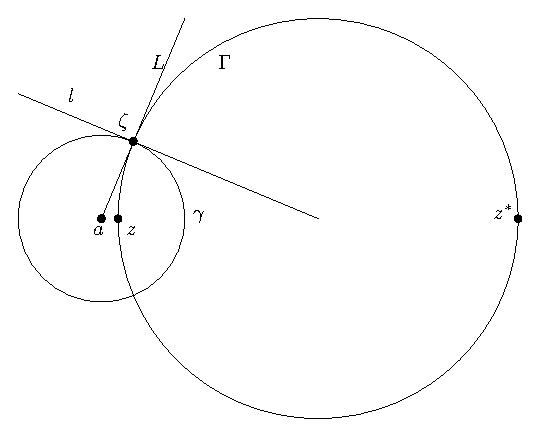
\includegraphics[scale=0.75]{neob.eps}
        \label{fig:23.1}
    \end{figure}
    Пусть $L$~--- касательная к $\Gamma$ из $a$, $\zeta \in L \cap \Gamma$.
    Тогда
    \begin{align*}
      & \left| a - \zeta \right|^2 = \left| a-z \right|\cdot \left| a-z^* \right| = R^2
    \end{align*}
    а значит, $\zeta \in \gamma$. Пусть $l$~--- касательная к $\Gamma$ в точке
    $\zeta$, $l \perp [a;\zeta] \Rightarrow l \perp L$.
    \item Достаточность.
    \begin{itemize}
        \item $\Gamma$~--- прямая, тогда $a \in \Gamma$, и значит, $z$ и $z^*$
        принадлежат одной полупрямой, исходящей из центра.
        \\
        Если точки лежат по разные стороны от центра, то построим окружность
        $\Gamma_1$ диаметром $zz^*$; тогда угол между $z$, точкой пересечения и
        $z^*$ равен $90^{\circ}$, а угол между $a$, точкой пересечения и центром
        окружности острый, т.~е. $L$ и $l$ не перпендикулярны).
            \begin{figure}[h!]
        \centering
        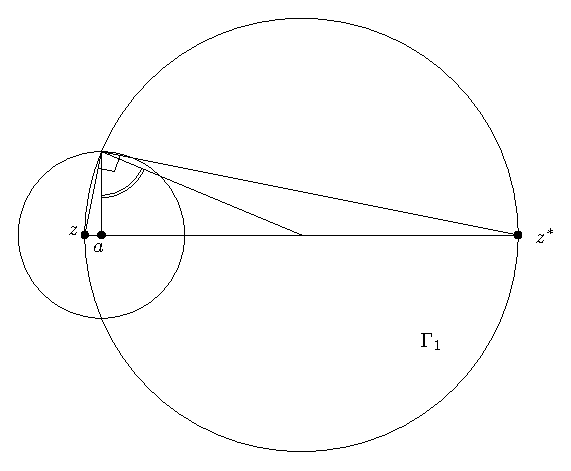
\includegraphics[scale=0.75]{dok.eps}
        \label{fig:23}
    \end{figure}
        \item $\Gamma$~--- окружность, тогда пусть $\zeta \in \Gamma \cap
        \gamma$, тогда
        \begin{align*}
          & \left| a - \zeta \right|^2 = \left| a-z \right|\cdot \left| a-z^* \right| = R^2
        \end{align*}
    \end{itemize}
\end{itemize}
\pr (теоремы)
$z$, $z^*$ симметричны относительно $\gamma$ (пусть окружности). Пусть $f$~---
ДЛО \eqref{(23.1)}, \eqref{(23.2)}. Пусть $w = f(z)$, $w^* = f(z^*)$, нужно
доказать, что они симметричны относительно $\tilde{\gamma} = f(\gamma)$.
\\
Рассмотрим $w$, $w^*$. Пусть $\tilde{\Gamma}$~--- любая окружность или прямая,
такая, что $w, w^* \in \tilde{\Gamma}$. Значит, по круговому свойству существует
окружность или прямая $\Gamma$: $\tilde{\Gamma} = f(\Gamma)$. По свойству
однолистности $z, z^* \in \Gamma$. Значит, по лемме $1$ $\gamma \perp \Gamma$.
Тогда, по свойству сохранения углов, $\tilde{\Gamma} \perp \tilde{\gamma}$. По
лемме $1$ тогда $w$ и $w^*$ симметричны относительно $\tilde{\Gamma}$.
\theorem
Множество ДЛО образует группу отображений относительно операции суперпозиции.
\pr
~
\begin{itemize}
    \item Очевидно, существует единичный элемент~--- тождественное отображение.
    \item У каждого ДЛО существует и единственно обратное ДЛО (см. теорему $1$).
    \item Суперпозиция ДЛО есть ДЛО. Действительно, пусть
    \begin{align*}
      & \zeta = \frac{a_1z+b_1}{c_1z+d_1}, \ w = \frac{a_2z+b_2}{c_2z+d_2}, \ a_1d_1 - c_1d_1 \neq 0, \ a_2d_2 - b_2c_2 \neq 0
    \end{align*}
    Положим
    \begin{align*}
      & z = \frac{z_1}{z_2}, \ \zeta = \frac{\zeta_1}{\zeta_2}, \ w = \frac{w_1}{w_2}
    \end{align*}
    Тогда
    \begin{align*}
      & \left( \begin{matrix}
              \zeta_1 \\
              \zeta_2
          \end{matrix} \right) = \left( \begin{matrix}
              a_1 & b_1 \\
              c_1 & d_1
          \end{matrix} \right) \cdot \left( \begin{matrix}
              z_1 \\
              z_2
          \end{matrix} \right), \ \left( \begin{matrix}
              w_1 \\
              w_2
          \end{matrix} \right) = \left( \begin{matrix}
              a_2 & b_2 \\
              c_2 & d_2
          \end{matrix} \right) \cdot \left( \begin{matrix}
              \zeta_1 \\
              \zeta_2
          \end{matrix} \right)
    \end{align*}
    \begin{align*}
      & \left( \begin{matrix}
              w_1 \\
              w_2
          \end{matrix} \right) = \left( \begin{matrix}
              a_2 & b_2 \\
              c_2 & d_2
          \end{matrix} \right) \cdot \left( \begin{matrix}
              a_1 & b_1 \\
              c_1 & d_1
          \end{matrix} \right) \cdot \left( \begin{matrix}
              z_1 \\
              z_2
          \end{matrix} \right)
    \end{align*}
    Получили невырожденное ДЛО.
\end{itemize}
\Example
Отобразить с помощью ДЛО области (см. рис.)
\begin{figure}[h!]
    \begin{minipage}[c]{0.45\textwidth}
        \centering
        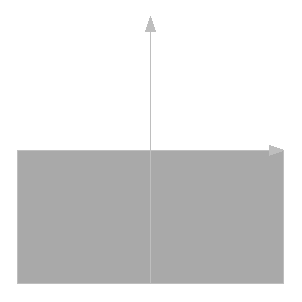
\includegraphics[scale=0.5]{half_plane.eps}
    \end{minipage}
    \begin{minipage}[c]{0.1\textwidth}
        \centering
        \LARGE{$\mapsto$}
    \end{minipage}
    \begin{minipage}[c]{0.45\textwidth}
        \centering
        
\includegraphics[scale=0.5]{round.eps}
    \end{minipage}
    \label{fig:23.2}
    \caption{$\Img z > 0 \mapsto \left| z \right| < 1$}
\end{figure}
\nonum
Возьмем любую $z_0: \ \Img z_0 > 0$. Пусть $z_0 \mapsto 0$, а $\ol{z_0} \mapsto
\infty$.
\\
Тогда
\begin{align*}
    & w = A\frac{z-z_0}{z-\ol{z_0}}
\end{align*}
Отыщем теперь $A$. Граница отображается на границу. Возьмем $x \in \RR$, она
должна отображаться на единичную окружность. Тогда
\begin{align*}
    & 1 = \abs{w} = \abs{A\frac{x-z_0}{x-\ol{z_0}}} = \left| A \right| \Rightarrow A = e^{i\alpha}
\end{align*}
Итак,
\begin{equation}\label{(23.6)}
    w = e^{i \alpha}\frac{z-z_0}{z-\ol{z_0}}
\end{equation}
\Example
Отобразить с помощью ДЛО области (см. рис.).
\\
\begin{figure}[h!]
    \begin{minipage}[c]{0.45\textwidth}
        \centering
        
\includegraphics[scale=0.5]{round.eps}
    \end{minipage}
    \begin{minipage}[c]{0.1\textwidth}
        \centering
        \LARGE{$\mapsto$}
    \end{minipage}
    \begin{minipage}[c]{0.45\textwidth}
        \centering
        
\includegraphics[scale=0.5]{round.eps}
    \end{minipage}
    \label{fig:23.3}
    \caption{$\left| z \right| < 1 \mapsto \left| z \right| < 1$}
\end{figure}
\nonum
Возьмем произвольную $z_0$ и отобразим ее в ноль; тогда симметричная $z_0^* =
\dst \frac{1}{\ol{z_0}}$ перейдет в $\infty$.
\\
Тогда
\begin{align*}
    & w = A\frac{z-z_0}{z-\dst \frac{1}{\ol{z_0}}} = \tilde{A}\frac{z-z_0}{1 - z\ol{z_0}}
\end{align*}
Граница перейдет в границу, а значит,
\begin{align*}
    & 1 = \abs{w} = \abs{\tilde{A}\frac{e^{i \varphi}-z_0}{1 - e^{i \varphi}\ol{z_0}}} = \abs{\tilde{A}\frac{e^{i \varphi}-z_0}{e^{-i \varphi}-\ol{z_0}}} = \abs{\tilde{A}}
\end{align*}
Итак,
\begin{equation}\label{(23.7)}
    w = e^{i \alpha}\frac{z-z_0}{1 - z\ol{z_0}}
\end{equation}
\Example
Отобразить с помощью ДЛО три различные точки $z_1, z_2, z_3$ в три точки $w_1,
w_2,w_3$.
\nonum
Заметим, что условиям удовлетворяет отображение вида
\begin{equation}\label{(23.8)}
    h(z) = \frac{z-z_1}{z-z_2} \cdot \frac{z_3-z_2}{z_3-z_1} = \frac{w-w_1}{w-w_2} \cdot \frac{w_3-w_2}{w_3-w_1} = g(w)
\end{equation}
\begin{align*}
  & w = f(z) = g^{-1}(h(z))
\end{align*}
Существование получено. Докажем единственность.
\\
Пусть для начала $f(z_k) = z_k$, тогда
\begin{align*}
  & \frac{az_k + b}{cz_k+d} = z_k
\end{align*}
\begin{align*}
  & cz^2_k + (d-a)z_k - b = 0
\end{align*}
Значит, поскольку квадратное уравнение имеет три решения, все его коэффициенты
равны нулю. Значит, $f(z) = z$.
\\
Пусть существуют $f_1(z)$, $f_2(z)$, причем $f_1(z_k) = f_2(z_k) = w_k$; тогда
$z_k = f_1^{-1}(f_2(z_k))$, тогда по групповому свойству $f_1^{-1}(z) =
f_2^{-1}(z)$, а значит, $f_1(z) = f_2(z)$.
\Example
Отобразить с помощью ДЛО области (см. рис.).
\\
\begin{figure}[h!]
    \begin{minipage}[c]{0.45\textwidth}
        \centering
        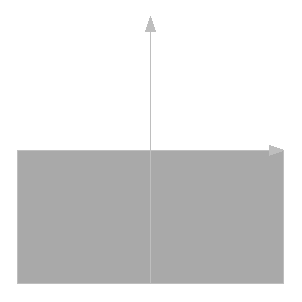
\includegraphics[scale=0.5]{half_plane.eps}
    \end{minipage}
    \begin{minipage}[c]{0.1\textwidth}
        \centering
        \LARGE{$\mapsto$}
    \end{minipage}
    \begin{minipage}[c]{0.45\textwidth}
        \centering
        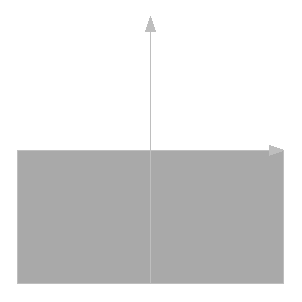
\includegraphics[scale=0.5]{half_plane.eps}
    \end{minipage}
    \label{fig:23.4}
    \caption{$\Img z > 0 \mapsto \Img z > 0$}
\end{figure}
\nonum
Пусть $x_1, x_2, x_3 \in \RR$, $x_1 < x_2 < x_3$, $u_1, u_2, u_3 \in \RR$, $u_1
< u_2 < u_3$, построим отображение $f(x_k) = u_k$. по примеру $3$ такое
отображение существует и единственно, границу оно переводит в границу. Из
свойства сохранения углов следует сохранение ориентации границы. Рассматривая
\eqref{(23.8)}, получаем все действительные  коэффициенты, т.~е. $a, b, c, d \in
\RR$, тогда $\forall x \in \RR \ \argm w'(x) = 0 \Rightarrow w'(x) > 0$, т.~е.
\begin{align*}
  & w'(x) = \frac{ad-cb}{(cx+d)^2} > 0 \Leftrightarrow ad-cb > 0
\end{align*}
Итак, необходимо и достаточно, чтобы все коэффициенты ДЛО были действительны,
причем $ad-cb > 0$.
\section{$\S 24.$ Конформные отображения элементарными функциями. Теорема Римама.}
Рассмотрим функции, обладающие локальной однолистностью.
\begin{center}
    \textbf{Степенная функция}
\end{center}
Фиксируем $t > 0$, рассмотрим область $G = \CC \setminus [0;+\infty)$. Пусть
\begin{align*}
  & w = \left| z \right|^t \exp(it \argt z), \ \argt z \in (0, 2 \pi)
\end{align*}
Функция регулярна при любом $t$. Действительно,
\begin{align*}
  & h(z) = \ln \left| z \right| + i \argt_0 z
\end{align*}
регулярна на этой области, а
\begin{align*}
  & w = \exp(t h(z))
\end{align*}
регулярна в этой области, как суперпозиция регулярных функций.
\\
Исследуем теперь однолистность. Рассмотрим
\begin{align*}
  & G_{0,\varphi_0} = \left\{ z \mid \left| z \right| > 0, \ \argt z \in (0; \varphi_0)\right\}
\end{align*}
\begin{align*}
  & l_{\varphi} = \left\{ z \mid z = r e^{i \varphi}, \ r > 0, \ \varphi \in (0, \varphi_0)\right\}
\end{align*}
Тогда
\begin{align*}
  & w(l_\varphi) = \left\{ w \mid w = \rho e^{i t \varphi}, \ \rho > 0 \right\}
\end{align*}
Тогда условие однолистности:
\begin{align*}
  & \begin{cases}
      0 < \varphi_0 < 2 \pi \\
      0 < t \varphi_0 < 2 \pi
  \end{cases}
\end{align*}
Значит, функция конформна на этой области.
\Example
$t = 2$, $w = z^2$.
\\
Условие однолистности: $\varphi_0 \in (0; \pi)$.
\begin{figure}[h!]
    \begin{minipage}[c]{0.45\textwidth}
        \centering
        
\includegraphics[scale=0.5]{half_round.eps}
    \end{minipage}
    \begin{minipage}[c]{0.1\textwidth}
        \centering
        \LARGE{$\mapsto$}
    \end{minipage}
    \begin{minipage}[c]{0.45\textwidth}
        \centering
        
\includegraphics[scale=0.5]{cut_rnd.eps}
    \end{minipage}
    \label{fig:24.1}
\end{figure}
\\
Заметим, что данный полукруг содержится в $G_{0, \pi}$~--- области
однолистности, значит, функция будет однолистна.
\Example
$t = 2$, $w = z^2$.
\\
Условие однолистности: $\varphi_0 \in (0; \pi)$.
\begin{figure}[h!]
    \begin{minipage}[c]{0.45\textwidth}
        \centering
        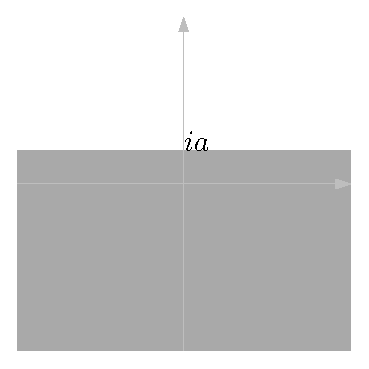
\includegraphics[scale=0.5]{top.eps}
    \end{minipage}
    \begin{minipage}[c]{0.1\textwidth}
        \centering
        \LARGE{$\mapsto$}
    \end{minipage}
    \begin{minipage}[c]{0.45\textwidth}
        \centering
        
\includegraphics[scale=0.5]{parabola.eps}
    \end{minipage}
    \label{fig:24.2}
\end{figure}
\\
Заметим, что данная полуплоскость содержится в $G_{0, \pi}$~--- области
однолистности, значит, функция будет однолистна. Зная, что граница переходит в
границу, отыщем $w(x+ia)$.
\begin{align*}
  & w(x+ia) = (x+ia)^2 = x^2 - a^2 + 2ixa
\end{align*}
\begin{align*}
  & \begin{cases}
      u = x^2 - a^2 \\
      v = 2xa
  \end{cases} \Rightarrow u  = \left( \frac{v}{2a} \right)^2 - a^2
\end{align*}
Поскольку $0$ не лежит в полуплоскости, искомая область будет внешностью
параболы.
\Example
$w = \left| z \right|^{\frac{1}{2}}\exp \left(\dst \frac{i}{2}\argt z\right)$.
\begin{figure}[h!]
    \begin{minipage}[c]{0.45\textwidth}
        \centering
        
\includegraphics[scale=0.5]{parabola.eps}
    \end{minipage}
    \begin{minipage}[c]{0.1\textwidth}
        \centering
        \LARGE{$\mapsto$}
    \end{minipage}
    \begin{minipage}[c]{0.45\textwidth}
        \centering
        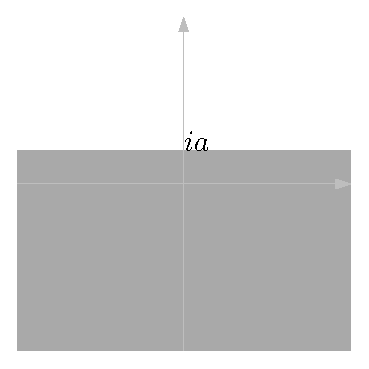
\includegraphics[scale=0.5]{top.eps}
    \end{minipage}
    \label{fig:24.3}
\end{figure}
Обратное к примеру $2$ отображение.
\begin{center}
    \textbf{Экспонента}
\end{center}
Всюду регулярна, но для однолистности необходимо, чтобы не было отличающихся на
$2 i \pi$ элементов (в силу периодичности).
\begin{figure}[h!]
    \centering
    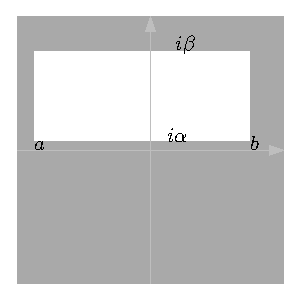
\includegraphics[scale=0.75]{odn_exp.eps}
    \label{fig:24.4}
    \caption{Область однолистности экспоненты}
\end{figure}
\begin{align*}
  & \begin{cases}
      -\infty \leq a \leq b \leq \infty \\
      0 \leq \beta - \alpha < 2 \pi
  \end{cases}
\end{align*}
\Example
\begin{figure}[h!]
    \begin{minipage}[c]{0.45\textwidth}
        \centering
        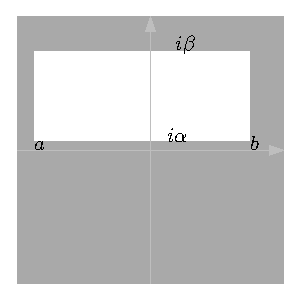
\includegraphics[scale=0.75]{odn_exp.eps}
    \end{minipage}
    \begin{minipage}[c]{0.1\textwidth}
        \centering
        \LARGE{$\mapsto$}
    \end{minipage}
    \begin{minipage}[c]{0.45\textwidth}
        \centering
        
\includegraphics[scale=0.5]{obraz_exp.eps}
    \end{minipage}
    \label{fig:24.5}
\end{figure}
Пусть $z = x+iy_0$, фиксированный $y_0 \in (\alpha,\beta)$. Тогда $\forall x \in
(a,b)$
\begin{align*}
  & f(z) = te^{iy_0}, \ t \in \left( e^{a}, e^{b} \right)
\end{align*}
\Example
~
\\
\begin{figure}[h!]
    \begin{minipage}[c]{0.45\textwidth}
        \centering
        
\includegraphics[scale=0.5]{polupolosa.eps}
    \end{minipage}
    \begin{minipage}[c]{0.1\textwidth}
        \centering
        \LARGE{$\mapsto$}
    \end{minipage}
    \begin{minipage}[c]{0.45\textwidth}
        \centering
        
\includegraphics[scale=0.5]{half_round.eps}
    \end{minipage}
    \label{fig:24.6}
    \caption{Перевод полуполосы в полуокружность.}
\end{figure}
Вертикальная черта переходит в полуокружность, верхняя граница~--- в отрезок
$[-1;0]$, нижняя граница~--- в отрезок $[0;1]$.
\Example
~
\\
\begin{figure}[h!]
    \begin{minipage}[c]{0.45\textwidth}
        \centering
        
\includegraphics[scale=0.5]{d_polupol.eps}
    \end{minipage}
    \begin{minipage}[c]{0.1\textwidth}
        \centering
        \LARGE{$\mapsto$}
    \end{minipage}
    \begin{minipage}[c]{0.45\textwidth}
        \centering
        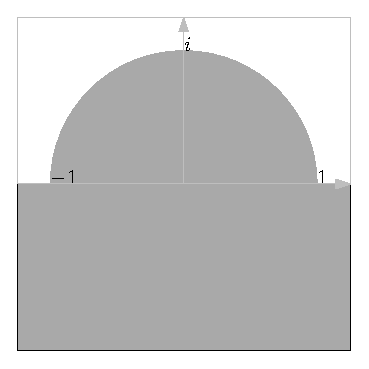
\includegraphics[scale=0.5]{out_rnd.eps}
    \end{minipage}
    \label{fig:24.7}
    \caption{Перевод полуполосы во внешность полуокружности.}
\end{figure}

    \begin{flushright}
    \textit{Лекция 19 (от 09.11)}
\end{flushright}
\begin{center}
    \textbf{Функция Жуковского}
\end{center}
\begin{equation}\label{(24.1)}
    w = \frac{1}{2}\left( z+\frac{1}{z} \right)
\end{equation}
Заметим, что $0$ и $\infty$~--- полюсы $1$ порядка, $\pm 1$~--- нули
производной.
\\
В каждой точке $z \not \in \left\{0, \pm 1,\infty \right\}$ функция конформна. В
точке $0$
\begin{align*}
  & g(z) = \frac{1}{w(z)} = \frac{2z}{z^2+1}
\end{align*}
Эта функция в нуле регулярна и имеет ненулевую производную, а значит, конформна
в нуле. В точке $\infty$
\begin{align*}
  & \varphi(z) = w\left( \frac{1}{z} \right) = \frac{1}{2}\left( \frac{1}{z} + z \right)
\end{align*}
Заметим, что это та же $w$, и в силу конформности в нуле конформна и на
бесконечности. В остальных точках проверим однолистность.
\begin{align*}
  & \frac{1}{2}\left( z_1 + \frac{1}{z_1} \right) - \frac{1}{2}\left( z_1 + \frac{1}{z_1} \right) = 0
\end{align*}
\begin{align*}
  & (z_1-z_2) \left( 1-\frac{1}{z_1z_2} \right)
\end{align*}
\begin{align*}
  & \left[ \begin{matrix}
          z_1=z_2 \\
          z_1z_2 = 1
      \end{matrix} \right.
\end{align*}
Область однолистности $G$: $\pm 1 \not \in G$, $\forall z \in G \ \dst
\frac{1}{z} \not \in G$.
\Example
Функция $w = \dst \frac{1}{z}$ задает две симметрии: относительно единичной
окружности и относительно действительной оси. Соответственно, области
однолистности:
\begin{itemize}
    \item $\left| z \right| < 1$
    \item $\left| z \right| > 1$
    \item $\Img z > 0$
    \item $\Img z < 0$
\end{itemize}
Пусть $z = e^{i \varphi}$, тогда функция Жуковского:
\begin{align*}
  & w = \frac{1}{2}\left( e^{i \varphi} + e^{-i\varphi}\right)
\end{align*}
\begin{equation}\label{(24.2)}
    \begin{cases}
        u = \frac{1}{2}\left( r+\frac{1}{r} \right)\cos \varphi \\
        v = \frac{1}{2}\left( r-\frac{1}{r} \right)\sin \varphi
    \end{cases}
\end{equation}
\Example
~
\begin{itemize}
    \item Пусть задана окружность
    \begin{align*}
      \gamma_r = \left\{ z: \left| z \right| = r, \ r \neq 1\right\}
    \end{align*}
    \begin{align*}
      & \frac{u^2}{a^2} + \frac{v^2}{b^2} = 1, \ a = \frac{1}{2}\left( r + \frac{1}{r} \right), \ b = \frac{1}{2}\left|  r - \frac{1}{r} \right|
    \end{align*}
    \begin{align*}
      & a^2+b^2 = c^2 = 1
    \end{align*}
    Такая окружность переходит в эллипс с фокусами в $\pm 1$, действительной
    полуосью $a$ и мнимой $b$.
    \item Пусть задан луч
    \begin{align*}
      l_\varphi = \left\{ z \mid z = re^{i\varphi}, \ r > 0\right\}, \ \varphi \in [-\pi;\pi) \setminus \left\{ 0, \pm \frac{\pi}{2}, -\pi \right\}
    \end{align*}
    \begin{equation}\label{(24.3)}
        \frac{u^2}{\cos^2 \varphi} - \frac{v^2}{\sin^2\varphi} = 1
    \end{equation}
    Такой луч переходит в гиперболу с фокусами в $\pm 1$.
    \begin{itemize}
        \item $\varphi \in \left( 0; \dst \frac{\pi}{2} \right)$~--- отображение
        в правую ветвь гиперболы, движение по ней вверх.
        \item $\varphi \in \left(\dst \frac{\pi}{2}; \pi \right)$~---
        отображение в левую ветвь гиперболы, движение по ней вверх.
        \item $\varphi \in \left( - \dst \frac{\pi}{2}; 0 \right)$~---
        отображение в правую ветвь гиперболы, движение по ней вниз.
        \item $\varphi \in \left( -\pi; -\dst \frac{\pi}{2} \right)$~---
        отображение в левую ветвь гиперболы, движение по ней вниз.
    \end{itemize}
\end{itemize}
\Example
~
\\
\begin{figure}[h!]
    \begin{minipage}[c]{0.45\textwidth}
        \centering
        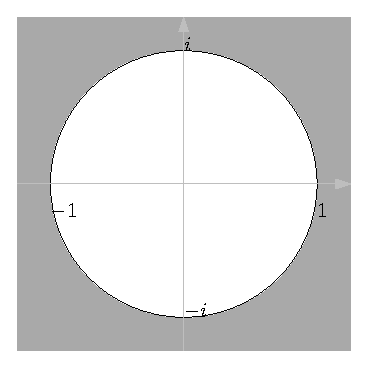
\includegraphics[scale=0.75]{rnd_in.eps}
    \end{minipage}
    \begin{minipage}[c]{0.1\textwidth}
        \centering
        \LARGE{$\mapsto$}
    \end{minipage}
    \begin{minipage}[c]{0.45\textwidth}
        \centering
        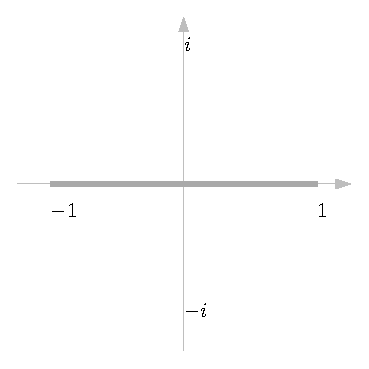
\includegraphics[scale=0.5]{pm1.eps}
    \end{minipage}
    \label{fig:24.10}
    \caption{Перевод единичного круга в $\CC \setminus [-1;1]$}
\end{figure}
\FloatBarrier
\Example
~
\\
\begin{figure}[h!]
    \begin{minipage}[c]{0.45\textwidth}
        \centering
        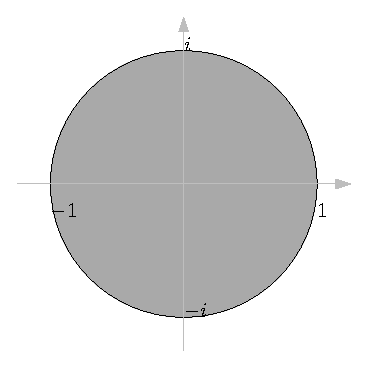
\includegraphics[scale=0.75]{rnd_out.eps}
    \end{minipage}
    \begin{minipage}[c]{0.1\textwidth}
        \centering
        \LARGE{$\mapsto$}
    \end{minipage}
    \begin{minipage}[c]{0.45\textwidth}
        \centering
        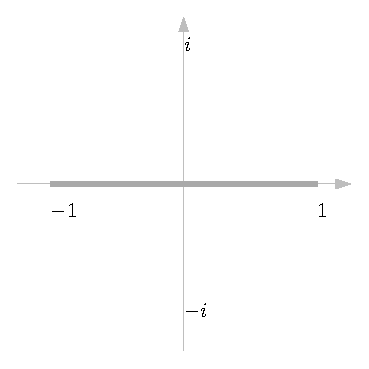
\includegraphics[scale=0.5]{pm1.eps}
    \end{minipage}
    \label{fig:24.11}
    \caption{Перевод внешности единичного круга в $\CC \setminus [-1;1]$}
\end{figure}
\FloatBarrier
\Example
~
\\
\begin{figure}[h!]
    \begin{minipage}[c]{0.45\textwidth}
        \centering
        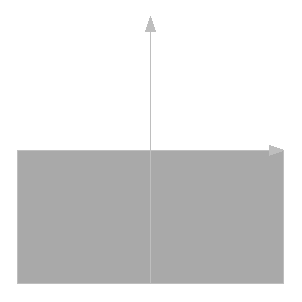
\includegraphics[scale=0.75]{half_plane.eps}
    \end{minipage}
    \begin{minipage}[c]{0.1\textwidth}
        \centering
        \LARGE{$\mapsto$}
    \end{minipage}
    \begin{minipage}[c]{0.45\textwidth}
        \centering
        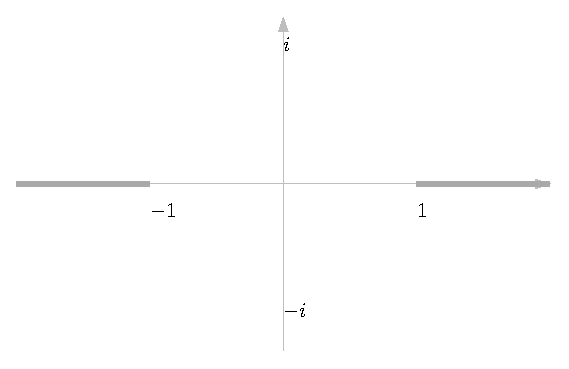
\includegraphics[scale=0.5]{pm1out.eps}
    \end{minipage}
    \label{fig:24.12}
    \caption{Перевод верхней полуплоскости в $\CC \setminus ((-\infty;-1]\cup[1;+\infty)$}
\end{figure}
\FloatBarrier
\Example
~
\\
\begin{figure}[h!]
    \begin{minipage}[c]{0.45\textwidth}
        \centering
        
\includegraphics[scale=0.75]{half_plane_t.eps}
    \end{minipage}
    \begin{minipage}[c]{0.1\textwidth}
        \centering
        \LARGE{$\mapsto$}
    \end{minipage}
    \begin{minipage}[c]{0.45\textwidth}
        \centering
        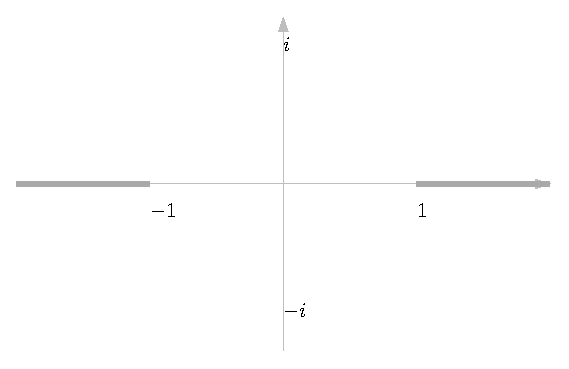
\includegraphics[scale=0.5]{pm1out.eps}
    \end{minipage}
    \label{fig:24.13}
    \caption{Перевод нижней полуплоскости в $\CC \setminus ((-\infty;-1]\cup[1;+\infty)$}
\end{figure}
\FloatBarrier
Отыщем обратную функцию Жуковского.
\begin{align*}
  & w = \frac{1}{2}\left( z+\frac{1}{z} \right) \Rightarrow z^2 - 2wz + 1 = 0
\end{align*}
\begin{align*}
  & z = w \pm g(w), \ g(w) \in \sqrt{w^2-1}
\end{align*}
\Example
Ветвь обратной функции Жуковского, где $g \sim w$ при $w \to \infty$, $z = w -
g(w)$, выполняет следующее преобразование:
\\
\begin{figure}[h!]
    \begin{minipage}[c]{0.45\textwidth}
        \centering
        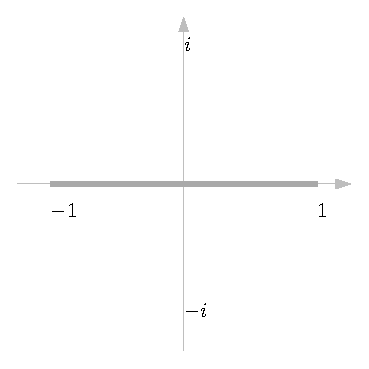
\includegraphics[scale=0.5]{pm1.eps}
    \end{minipage}
    \label{fig:24.14}
    \begin{minipage}[c]{0.1\textwidth}
        \centering
        \LARGE{$\mapsto$}
    \end{minipage}
        \begin{minipage}[c]{0.45\textwidth}
        \centering
        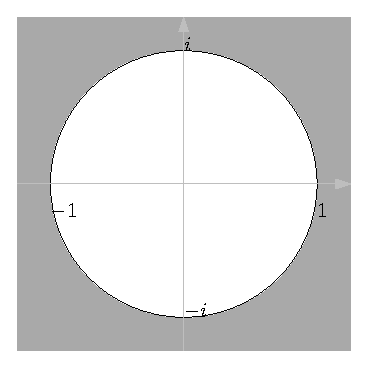
\includegraphics[scale=0.75]{rnd_in.eps}
    \end{minipage}
    \caption{Перевод $\CC \setminus [-1;1]$ в единичный круг}
\end{figure}
\FloatBarrier
\Example
Ветвь обратной функции Жуковского, где $g \sim w$ при $w \to \infty$, $z = w +
g(w)$, выполняет следующее преобразование:
\\
\begin{figure}[h!]
        \begin{minipage}[c]{0.45\textwidth}
        \centering
        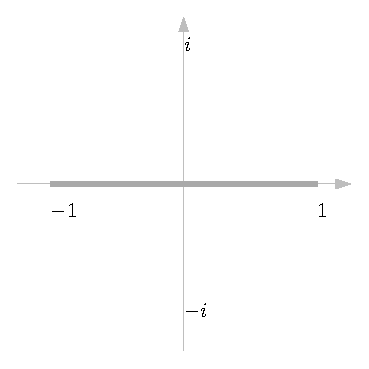
\includegraphics[scale=0.5]{pm1.eps}
    \end{minipage}
    \begin{minipage}[c]{0.1\textwidth}
        \centering
        \LARGE{$\mapsto$}
    \end{minipage}
        \begin{minipage}[c]{0.45\textwidth}
        \centering
        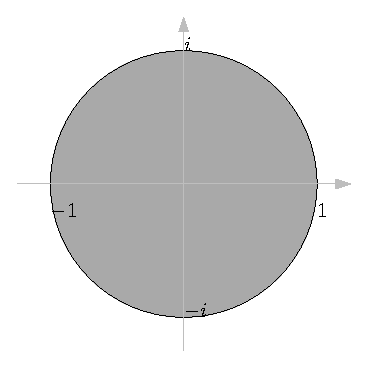
\includegraphics[scale=0.75]{rnd_out.eps}
    \end{minipage}
    \label{fig:24.15}
    \caption{Перевод $\CC \setminus [-1;1]$ во  внешность единичного круга}
\end{figure}
\FloatBarrier
\Example
Ветвь обратной функции Жуковского, где $g(0) = i$, $z = w - g(w)$, выполняет
следующее преобразование:
\\
\begin{figure}[h!]
        \begin{minipage}[c]{0.45\textwidth}
        \centering
        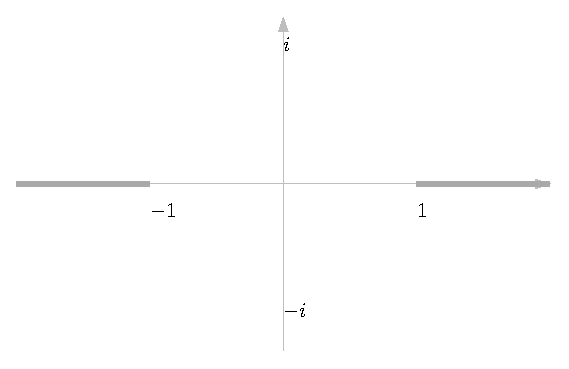
\includegraphics[scale=0.5]{pm1out.eps}
    \end{minipage}
    \begin{minipage}[c]{0.1\textwidth}
        \centering
        \LARGE{$\mapsto$}
    \end{minipage}
    \begin{minipage}[c]{0.45\textwidth}
        \centering
        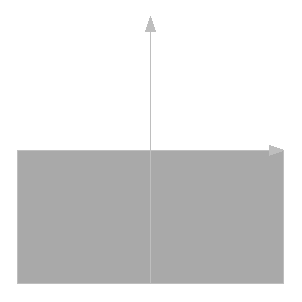
\includegraphics[scale=0.75]{half_plane.eps}
    \end{minipage}
    \label{fig:24.16}
    \caption{Перевод $\CC \setminus (-\infty;-1]\cup[1;+\infty)$ в верхнюю полуплоскость}
\end{figure}
\FloatBarrier
\Example
Ветвь обратной функции Жуковского, где $g(0) = i$, $z = w + g(w)$, выполняет
следующее преобразование:
\\
\begin{figure}[h!]
        \begin{minipage}[c]{0.45\textwidth}
        \centering
        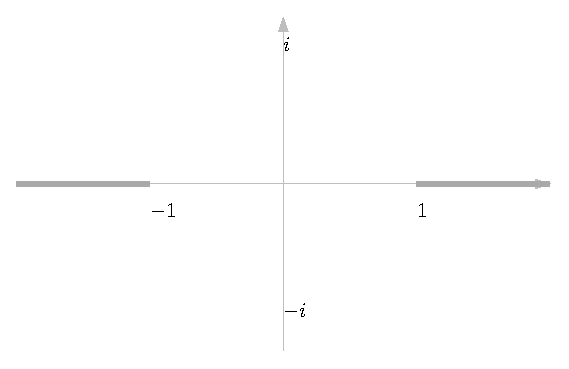
\includegraphics[scale=0.5]{pm1out.eps}
    \end{minipage}
    \begin{minipage}[c]{0.1\textwidth}
        \centering
        \LARGE{$\mapsto$}
    \end{minipage}
    \begin{minipage}[c]{0.45\textwidth}
        \centering
        
\includegraphics[scale=0.75]{half_plane_t.eps}
    \end{minipage}
    \label{fig:24.17}
    \caption{Перевод $\CC \setminus (-\infty;-1]\cup[1;+\infty)$ в нижнюю полуплоскость}
\end{figure}
\FloatBarrier
\begin{center}
    \textbf{Теорема Римана}
\end{center}
$\CC$ нельзя конформно отобразить на единичный круг. Действительно, функция (в
предположении существования) будет ограничена, регулярна (в силу определенности
на всей комплексной плоскости она обязана быть целой), значит, по теореме
Лиувилля это константа, что не является требуемым отображением.
\theorem
Общий вид конформного отображения $B_1(0) \mapsto B_1(0)$:
\begin{equation}\label{(24.4)}
    f(z) = e^{i\beta}\frac{z-a}{1-z\ol{a}}
\end{equation}
\pr
Если $f$ удовлетворяет \eqref{(24.4)}, то $f: B_1(0) \mapsto B_1(0)$ есть ДЛО, а
значит, оно конформно.
\\
Пусть теперь $g: B_1(0) \mapsto B_1(0)$~--- некоторое конформное отображение.
Докажем, что такая функция удовлетворяет \eqref{(24.4)}.
\\
Заметим:
\begin{align*}
  \exists w_0 \in B_1(0): \ g(0) = w_0
\end{align*}
Расмотрим теперь
\begin{align*}
  h(w) = \frac{w-w_0}{1-w\ol{w_0}}, \ h(w_0) = 0, \ h:B_1(0)\mapsto B_1(0)
\end{align*}
Положим
\begin{align*}
  f(z) = h(g(z))
\end{align*}
$f$ регулярна, как суперпозиция регулярных функций, и причем $f(0) = 0$,
$f:B_1(0) \mapsto B_1(0)$. Тогда по лемме Шварца $\forall z \in B_1(0) \ \left|
    f(z) \right|\leq \left| z \right|$.
\\
Тогда $f^{-1}$ таже будет регулярна, $f^{-1}(0) = 0$, $f^{-1}: B_1(0) \mapsto
B_1(0)$. Тогда по лемме Шварца $\forall w \in B_1(0) \ \left| f^{-1}(w)
\right|\leq \left| w \right|$. Подставляя сюда $w = f(z)$, получим $\left| z
\right| \leq \left| f(z) \right|$, т.~е. $\left| z \right| = \left| f(z)
\right|$, и по лемме Шварца выполняется $f(z) = e^{i\alpha}z$.
\\
Тогда $g(z)$~--- ДЛО. Проверим, что $g$ имеет вид \eqref{(24.4)}.
\begin{align*}
& e^{i\alpha}z = h^{-1}(g(z)); \ \exists z_0 \in B_1(0): \ g(z_0) = 0
\end{align*}
\begin{align*}
& e^{i\alpha} = (h^{-1})'(0)(g'(z_0)) = \frac{g'(z_0)}{h'(w_0)}
\end{align*}
\begin{align*}
& \alpha \in \Arg g'(z_0) - \Arg h'(w_0)
\end{align*}
\begin{align*}
& h'(w_0) = \left.\frac{1-w\ol{w_0}+\ol{w_0}(w-w_0)}{(1-w\ol{w_0})^2}\right|_{w=w_0} = 1 - \left| w_0 \right|^2 > 0 \Rightarrow 0 \in \Arg h'(w_0)
\end{align*}
\begin{align*}
& \alpha \in \Arg g'(z_0)
\end{align*}
Рассмотрим теперь 
\begin{align*}
& g_1(z) = e^{i\alpha}\frac{z-z_0}{1-z\ol{z_0}}
\end{align*}
\begin{align*}
&\varphi(z) = g(g_1^{-1}(w)): B_1(0) \mapsto B_1(0)
\end{align*}
\begin{align*}
&\varphi(g_1(z)) = g(w), \ \varphi(0) = 0, \ \Arg \varphi'(0) + \Arg g_1'(0) = \Arg g'(z_0)
\end{align*}
Дифференцируя,
\begin{align*}
& \alpha \in \Arg g_1(0), \ 0 \in \Arg \varphi'(0)
\end{align*}
По лемме Шварца для прямой и обратной функций
\begin{align*}
& \left| \varphi(z) \right| = \left| z \right| \Rightarrow \varphi(z) = z
\end{align*}
(в силу $0 \in \Arg \varphi'(0)$). Но тогда $g_1(z) = g(z)$, и теорема
доказана.
\lemma 
Пусть область $G\subseteq \CC$ такова, что существует конформное $f_0: G \mapsto
B_1(0)$. Тогда любое конформное отображение $G$ на $B_1(0)$ имеет вид
\begin{align*}
  & f(z) = h(f_0(z))
\end{align*}
причем $h$ имеет вид \eqref{(24.4)}.
\pr
Пусть $f_1: G \mapsto B_1(0)$~--- конформное. Рассмотрим 
\begin{align*}
  & \varphi(w) = f_1(f_0^{-1}(w)): B_1(0) \mapsto B_1(0)
\end{align*}
Оно конформно как суперпозиция конформных. По теореме $1$ это ДЛО,
уловлетворяющее \eqref{(24.4)}. Поскольку
\begin{align*}
& f_1(z) = \varphi(f_0(z))
\end{align*}
то лемма доказана.
\theorem (единственности конформных отображений)
Пусть $G$ такова, что существует конформное $f_0:G \mapsto B_1(0)$. Тогда
множество всех конформных отображений $G \mapsto B_1(0)$ зависит от трех
действительных параметров. В частности, такое отображение единственно, если
выполнены условия:
\begin{equation}\label{(24.5)}
f(z_0) = 0, \ \argt f'(z_0) = \alpha \in [0;2\pi), \ z_0 \in G
\end{equation}
\pr
Из леммы $1$ и теоремы $1$ следует утверждение о трех параметрах.
\\
Докажем теперь единственность. Допустим, от противного, существуют $f_1$, $f_2$,
удовлетворяющие \eqref{(24.5)}. Пусть
\begin{align*}
  & \varphi(w) = f_1(f_2^{-1}(w)), \ \varphi(f_2(z)) = f_1(z), \ \varphi(0) = 0
\end{align*}
Значит, $\varphi(z)$ будет ДЛО по лемме $1$. Дифференцируя в $z_0$, имеем
\begin{align*}
    & \argt \varphi'(0) + \Arg f_2'(z_0) = \Arg f_1'(z_0)
\end{align*}
\begin{align*}
  & 0 \in \Arg \varphi'(0) \Rightarrow \varphi(0) = 0, \ z_0 = 0, \ \alpha = 0
\end{align*}
\begin{align*}
  & \varphi(z) = z \Rightarrow f_1(z) = f_2(z)
\end{align*}
\theorem (Римана)
Пусть $G$~--- область в $\CCC$, граница которой содержит более одной точки.
Тогда существует конформное $f: G \mapsto B_1(0)$.
\corollary
Если $G_1 \subseteq \CCC$, $G_2 \subseteq \CCC$, и ганицы каждой содержат более
одной точки, то существует конформное обображение $G_1$ на $G_2$.
\pr
Пусть $f_1: G_1 \mapsto B_1(0)$, $f_2: G_2 \mapsto B_1(0)$, тогда искомое
отображение $\varphi(z) = f_1(f_2^{-1}(z)): G_1 \mapsto G_2$.
\theorem (принцип соответствия границ)
Пусть $G_1, G_2$~--- ограниченные односвязные области в $\CC$ с кусочно гладкими
границами $\Gamma_1, \Gamma_2$. Пусть $f: G_1 \mapsto G_2$~--- конформное; тогда
существует непрерывное продолжение $\tilde{f}$ такое, что оно отображает
$\Gamma_1$ на $\Gamma_2$ с сохранением ориентации.
    \begin{flushright}
    \textit{Лекция 20 (от 10.11)}
\end{flushright}
\section{$\S 25.$ Принцип симметрии.}
\theorem
Пусть заданы области $G$, $G^*$ в верхней полуплоскости с кусочно гладкими
границами $\Gamma$, $\Gamma^*$. Пусть границы содержат конечное чило интервалов
действительной оси $l_1, \dots, l_n$, $l_1^*, \dots, l_n^*$. Пусть $\tilde{G}$,
$\tilde{G^*}$~--- симметричные относительно действительной оси области. Пусть
$f: G \cup \dst \bigcup_{s=1}^n l_s \mapsto G^*\cup \dst \bigcup_{s=1}^n l_s^*$
конформна на $G$ и непрерывна на $G \cup \dst \bigcup_{s=1}^n l_s$ взамно
однозначно отображает $\forall s \in \left\{ 1, \dots, n \right\} \ l_s \mapsto
l_s^*$. Тогда существует (аналитическое) продолжение $f$ на область $G \cup \dst
\bigcup_{s=1}^n l_s \cup \tilde{G}$, конформно отображающее ее на $G^* \cup \dst
\bigcup_{s=1}^n l_s^* \cup \tilde{G^*}$.
\begin{figure}[h!]
    \begin{minipage}[c]{0.5\textwidth}
        \centering
        
\includegraphics[scale=0.75]{1st.eps}
    \end{minipage}
    \begin{minipage}[c]{0.5\textwidth}
        \centering
        
\includegraphics[scale=0.75]{2nd.eps}
    \end{minipage}
    \label{fig:25.1}
\end{figure}
\pr
Зададим функцию $F$ (искомое продолжение).
\begin{equation}\label{(25.1)}
    F(z) = \begin{cases}
        f(z), \ z \in G \cup \bigcup_{s=1}^n l_s \\
        \ol{f(\ol{z})}, \ z \in \tilde{G}
    \end{cases}
\end{equation}
Докажем дифференцируемость. Пусть $z_0 \in \tilde{G}$; тогда
\begin{align*}
  & \exists \varepsilon > 0: \ \forall \Delta z: \ \left| \Delta z \right| < \varepsilon \ z_0+\Delta z \in G
\end{align*}
\begin{align*}
  & \frac{F(z_0+\Delta z) - F(z_0)}{\Delta z} = \frac{\ol{f}(\ol{z_0+\Delta z}) - \ol{f}(\ol{z_0})}{\Delta z} = \ol{\frac{f(\ol{z_0}+\ol{\Delta z}) - f(\ol{z_0})}{\ol{\Delta z}}}
\end{align*}
Тогда
\begin{align*}
  & \ol{z_0} \in G, \ \ol{z_0} +\ol{\Delta z} \in G, \ \exists f'(\ol{z_0}) = \lim_{\Delta z \to 0} \frac{f(\ol{z_0}+\ol{\Delta z}) - f(\ol{z_0})}{\ol{\Delta z}}
\end{align*}
\begin{align*}
  & \exists F'(z_0) = \ol{f'(\ol{z_0})}
\end{align*}
Пусть теперь $x_0 \in l_s$. Докажем, что $F(z)$ непрерывна в $x_0$. Рассмотрим
нижний полукруг окрестности.
\begin{align*}
  & \lim_{z \os{\tilde{G}}{\to} x_0}F(z) = \lim_{\ol{z} \os{G}{\to} x_0}\ol{f(\ol{z})} = \ol{\lim_{\ol{z} \os{G}{\to} x_0}f(\ol{z})} = \ol{f(x_0)} = f(x_0) \in l_s^*
\end{align*}
Аналогично находится предел по верхнему полукругу.
\\
Тогда по теореме о стирании разреза $F(z)$ регулярна в $x_0$ и, значит,
регулярна во всей объединенной области.
\\
Докажем, наконец, однолистность. Область $G$ отображалась однолистно, как и
интервалы; каждая точка $\tilde{G}$ соответствует единственной точке $G$, как и
$\tilde{G^*}$ и $G^*$, а значит, отображение однолистно и на оставшейся части.
\corollary
принцип симметрии можнообобщить на симметрии относительно любой прямой или
окружности.
\pr
Всякую такую кривую можем перевести в действительную ось (область~--- в верхнюю
полуплоскость), применить принцип симметрии и перевести обратно.
\Example
Найти преобразование, переводящее данные области.
\begin{figure}[h!]
    \begin{minipage}[c]{0.45\textwidth}
        \centering
        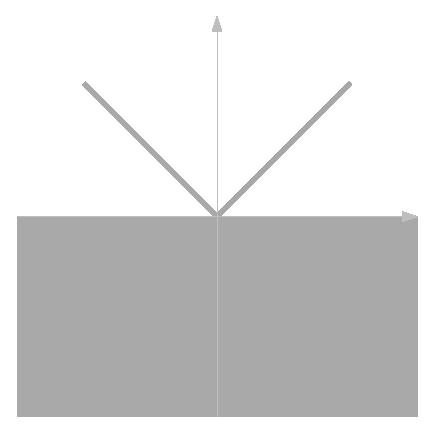
\includegraphics[scale=0.75]{ex24_1.eps}
    \end{minipage}
    \begin{minipage}[c]{0.1\textwidth}
        \centering
        \LARGE{$\mapsto$}
    \end{minipage}
    \begin{minipage}[c]{0.45\textwidth}
        \centering
        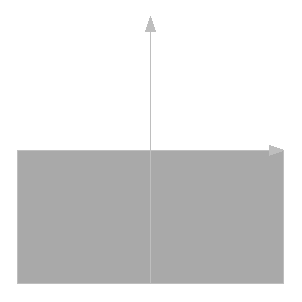
\includegraphics[scale=0.5]{half_plane.eps}
    \end{minipage}
    \label{fig:25.1}
\end{figure}
Воспользовавшись принципом симметрии, рассмотрим лишь правую часть вместе с
мнимой осью. Используя $w_1 = z^4$, получим $\CC \setminus[-4;+\infty)$, причем
функция будет непрерывно продлена на нижний край разреза от нуля и до
бесконечности. Применяя $w_2 = w_1+4$, получим $\CC \setminus[0;+\infty)$, причем
функция будет непрерывно продлена на нижний край разреза от $4$ и до
бесконечности. При помощи $w_3 = \sqrt{\left| w_2 \right|}\exp \left(
\dst \frac{i}{2}\argt w_2\right)$ получаем верхнюю полуплоскость, а $(-\infty;
-2]$ имеет непрерывное продолжение функции на себе. Затем сдвигаем этот разрез:
$w_4 = w_3+2$, и извлекаем корень: $w_5 = \sqrt{\left| w_4 \right|}\exp \left(
    \dst \frac{i}{2}\argt w_4\right)$. По принципу симметрии можем раскрыть все
до полуплоскости.
\begin{center}
    \begin{tabular}{cccc}
      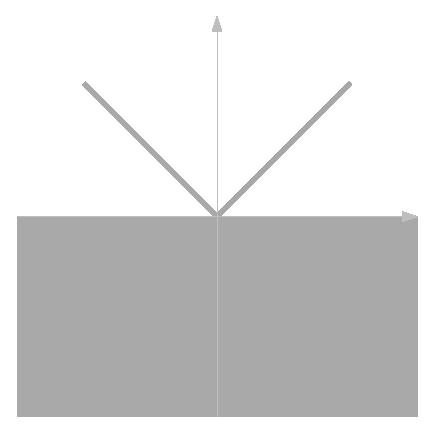
\includegraphics[scale=0.75]{ex24_1.eps} & $\Rightarrow$ & 
\includegraphics[scale=0.75]{2511.eps} & $\mapsto$ \\
    \end{tabular}
\end{center}
\begin{center}
    \begin{tabular}{cccc}
      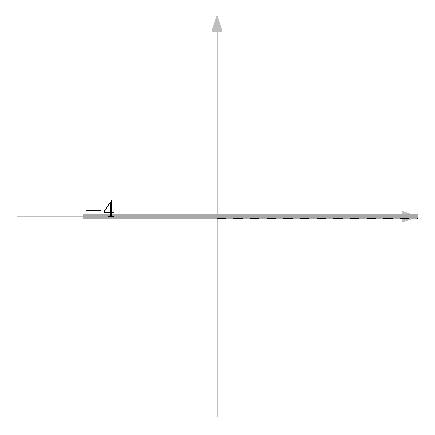
\includegraphics[scale=0.75]{2512.eps} & $\mapsto$ & \includegraphics[scale=0.75]{2513.eps} & $\mapsto$ \\
    \end{tabular}
\end{center}
\begin{center}
    \begin{tabular}{cccc}
      \includegraphics[scale=0.75]{2514.eps} & $\mapsto$ & \includegraphics[scale=0.75]{2515.eps} & $\mapsto$ \\
    \end{tabular}
\end{center}
\begin{center}
    \begin{tabular}{cccc}
      \includegraphics[scale=0.75]{2516.eps} & $\Rightarrow$ & \includegraphics[scale=1]{half_plane.eps} & \\
    \end{tabular}
\end{center}
\Example
Найти преобразование, переводящее данные области.
\begin{align*}
  & G = \left\{ z = x+iy \mid y^2 < 2p \left( x+\frac{p}{2} \right) \right\}, \ p > 0
\end{align*}
\begin{figure}[h!]
    \begin{minipage}[c]{0.45\textwidth}
        \centering
        \includegraphics[scale=0.75]{2520.eps}
    \end{minipage}
    \begin{minipage}[c]{0.1\textwidth}
        \centering
        \LARGE{$\mapsto$}
    \end{minipage}
    \begin{minipage}[c]{0.45\textwidth}
        \centering
        \includegraphics[scale=0.5]{half_plane.eps}
    \end{minipage}
    \label{fig:25.1}
\end{figure}
Воспользовавшись принципом симметрии, рассмотрим лишь верхнюю часть вместе с
действительной осью. Используя $w_1 = \sqrt{\left| z \right|}\exp \left(\dst
    \frac{i}{2}\argt z\right)$, получаем полуполосу. Растянем эту полуполосу при
помощи $w_2 = \pi\sqrt{\frac{2}{\pi}}$, экспонентой $w_3 = e^{w_2}$ превратим в
верхнюю полуплоскость с вырезанным единичным полукругом. Функцией Жуковского
$w_4 = dst \frac{1}{2}\left( w_3+\dst\frac{1}{w_4} \right)$ переводим в верхнюю
полуплоскость, но она имеет особый участок $[-1;+\infty)$. По принципу симметрии
можем раскрыть это до плоскости с разрезом по $(-\infty;-1]$, и легко, сдвигая
$w_5 = -w_4+1$ и извлекая корень $w_6 = \sqrt{\left| w_5 \right|}\exp \left(\dst
    \frac{i}{2}\argt w_5\right)$, получаем искомое.
\begin{center}
    \begin{tabular}{cccc}
      \includegraphics[scale=0.75]{2520.eps} & $\Rightarrow$ & \includegraphics[scale=0.75]{2521.eps} & $\mapsto$ \\
    \end{tabular}
\end{center}
\begin{center}
    \begin{tabular}{cccc}
      \includegraphics[scale=0.75]{2522.eps} & $\mapsto$ & \includegraphics[scale=0.75]{2523.eps} & $\mapsto$ \\
    \end{tabular}
\end{center}
\begin{center}
    \begin{tabular}{cccc}
      \includegraphics[scale=0.75]{2524.eps} & $\mapsto$ & \includegraphics[scale=0.75]{2525.eps} & $\Rightarrow$ \\
    \end{tabular}
\end{center}
\begin{center}
    \begin{tabular}{cccc}
      \includegraphics[scale=0.75]{2526.eps} & $\mapsto$ & \includegraphics[scale=1]{2527.eps} & $\mapsto$ \\
    \end{tabular}
\end{center}
\begin{center}
    \begin{tabular}{cccc}
      \includegraphics[scale=0.5]{half_plane.eps} & & & \\
    \end{tabular}
\end{center}
\section{$\S 26.$ Задача Дирихле на плоскости.}
\theorem
Пусть $f: G \mapsto D$ регулярная и непрстоянная. Пусть $\tilde{u}: D \mapsto
\RR$ гармоническая. Тогда $u(z) = \tilde{u}(f(z))$ также гармоническая.
\pr
Пусть $z_0 \in G$~--- произвольная точка. Пусть $f(z_0) = w_0$, и $f(G) =
G^*$~--- также, как известно, область. Тогда
\begin{align*}
  & \exists \varepsilon > 0: B_\varepsilon(w_0) \subseteq G^* \subseteq D
\end{align*}
По теореме $2$ $\S 4$
\begin{align*}
  & \exists h(w): \ \Real h(w) = \tilde{u}(w), \ w \in B_\varepsilon(w_0)
\end{align*}
причем $h$~--- регулярная. Рассмотрим теперь $h(f(z))$ в окрестности
$B_\delta(w_0)$, такой, чо $f\left( B_\delta(z_0) \right) \subseteq
B_\varepsilon(w_0)$. Тогда в этой окрестности $h$ будет регулярной,
$\tilde{u}(w) = \Real h(w)$~--- гармонической, тогда и $u(z) = \tilde{u}(f(z))$
тоже будет гармонической в этой окрестности, а в силу произвольности выбора
$z_0$~--- и на всей области.
\Def
\textbf{Классическим решением задачи Дирихле в области $G$} называется
следующее:
\begin{itemize}
    \item $G$~--- ограниченная односвязная область в $\CC$ с кучочно гладкой
    границей $\Gamma$;
    \item дана непрерывная функция $u_0(z)$ на этой границе;
    \item нужно найти гармоническую функцию $u(z)$ в области $G$, непрерывную на
    ее замыкании и удовлетворяющую условию: $u\Big|_\Gamma = u_0$.
\end{itemize}
\Def
\textbf{Общей задачей Дирихле} называется следующее:
\begin{itemize}
    \item $G$~--- односвязная область в $\CCC$ с кучочно гладкой границей $\Gamma$;
    \item дана непрерывная функция всюду за исключением коненого числа точек
    разрыва $1$ рода $\zeta_1, \dots, \zeta_n$ $u_0(z)$ на этой границе и
    ограниченная на ней за вычетом этих точек;
    \item нужно найти гармоническую функцию $u(z)$ в области $G$, ограниченную
    на ее замыкании, непрерывную на ее замыкании за вычетом этих точек и
    удовлетворяющую условию: $u = u_0$ на границе за вычетом этих точек.
\end{itemize}
\lemma
Лемма доказывается для случая ограниченной области.
\\
Пусть $G$~--- ограниченная односвязная область в $\CC$. Если решение общей
задачи Дирихле существует в этой области с $u_0(z)$ и $\tilde{\Gamma} = \Gamma
\setminus \dst \bigcup_{k=1}^n \left\{ \zeta_k \right\}$, то все значения $u(z)$
лежат на отрезке $\left[ m, M \right]$, где $m = \us{z \in\tilde{\Gamma}}{\inf} u_0(z)$, $M = \us{z \in\tilde{\Gamma}}{\sup}u_0(z)$.
\pr
Пусть $d = \sup \left| z_1-z_2 \right|$, $z_1, z_2 \in G$~--- диаметр множества.
Пусть
\begin{equation}\label{(26.1)}
    U_\varepsilon = M + \varepsilon \sum_{k=1}^n \ln \frac{d}{\left| z-\zeta_k\right|}, \ \varepsilon > 0
\end{equation}
Это гармоническая функция, причем она не меньше $M$ и непрерывна на замыкании
за вычетом точек разрыва, причем
\begin{equation}\label{(26.2)}
    \lim_{z \to \zeta_k} U_\varepsilon(z) = \infty
\end{equation}
Полагая
\begin{align*}
  & \gamma_r^k = \left\{ z \in G: \left| z - \zeta_k \right| = r\right\}
\end{align*}
\begin{equation}\label{(26.3)}
    \lim_{r \to 0}\min \left\{ U_\varepsilon(z) \mid z \in \gamma_r^k \right\} = +\infty
\end{equation}
\begin{align*}
    & \forall z \in \tilde{\Gamma} \ U_\varepsilon(z) > M\geq u_0(z) = u(z)
\end{align*}
Из ограниенности и выполнимости \eqref{(26.3)} для $u(z)$ имеем, чтопри
достаточно малых $r$ на границе области $G_r = G \setminus \dst \bigcup_{k=1}^n
B_r(\zeta_k)$ $U_\varepsilon(z) > U(z)$. По принципу максмума гармонической
функции это соотношение верно и для всей $G_r$.
\\
Фиксируем произвольную  $z \in G$. тогда $\exists r_0: z \in G_{r_0}$, значит,
$U_\varepsilon(z) > u(z)$ на всей $G$. При устремлении $\varepsilon$ к нулю
получаем, что $u(z) \leq M$.
\\
Аналогично можем ограничить сверху гармоническую $-u(z)$ числом $-m$ и получить
искомое.
\Note
Без условия ограниченности области лемма также справедлива.
\corollary
Для случая непостоянной $u_0(z)$ выполняются строгие неравенства.
\pr
От противного: предположим существование внутренней точки области, где $M$
достигается; тогда должна существовать $z_1 \in G: \ u(z_1) > M$ (аналогичнно
доказательству принципа максимума). Противоречие с неравенством, даже нестрогим.    

    \begin{flushright}
    \textit{Лекция 21 (от 16.11)}
\end{flushright}
\theorem
В общей задаче Дирихле при существовании решения в ограниченной области онобудет
единственным. Решение ищем как ограниченную функцию.
\pr
От противного. Допустим, существуют два различных решения $u_1$, $u_2$. Тогда $w
= u_1-u_2 : G \mapsto \RR$, $\Delta w = 0$, $w\Big|_\Gamma = 0$. Тогда по лемме
$1$ $w \equiv 0$.
\Note
Условие ограниченности области является лишь техническим. Условие же
ограниченности функции на области существенно.
\Example
\begin{align*}
  & u(x,y) = \frac{x^2+y^2-2x}{x^2+y^2}
\end{align*}
\begin{align*}
  & G = \left\{ (x,y) \mid x^2+y^2<2x \right\} = \left\{ z: \left| z \right| <1\right\}
\end{align*}
При граничном условии~--- нуле эта функция является решением задачи Дирихле, но
и тождественный нуль также решение. При условии ограниченности эта функция не
подходит.
\begin{center}
    \textbf{Класическая задача Дирихле в круге $B_R(0), \ R > 0$}
\end{center}
\begin{equation}\label{(26.4)}
    \begin{cases}
        \Delta u = 0, \ \left| z \right|< R \\
        u \big|_{\left| z \right| = R} = u_0(z)
    \end{cases}
\end{equation}
причем $u_0(z)$ непрерывна на $\gamma_r$ и решение \eqref{(26.4)} непрерывно на
некотором $B_{R_1}(0), \ R_1 > R$.
\\
Тогда существует регулярная $f: B_{R_1}(0) \mapsto \CC$, что $\Real f(z) =
u(z)$. Тогда по интегральной формуле Коши
\begin{align*}
  & \forall z \in B_R(0) \ f(z) = \frac{1}{2 i \pi} \int_{\gamma_R} \frac{f(\zeta)}{\zeta - z}d\zeta = \frac{1}{2 \pi} \int_{0}^{2\pi} \frac{f(Re^{i\psi})\zeta(\psi)}{\zeta(\psi) - z}d\psi
\end{align*}
Введем теперь симметричную точку $z^* = \dst \frac{R^2}{z}$. Тогда
\begin{align*}
  & \frac{1}{2 i \pi} \int_{\gamma_R} \frac{f(\zeta)}{\zeta - z^*}d\zeta = \frac{1}{2 \pi} \int_{0}^{2\pi} \frac{f(Re^{i\psi})\zeta(\psi)}{\zeta(\psi) - z^*}d\psi = 0
\end{align*}
\begin{align*}
  & f(z) = \frac{1}{2\pi}\int_{0}^{2\pi}f(\zeta(\psi))\left( \frac{\zeta(\psi)}{\zeta(\psi) - z} - \frac{\zeta(\psi)}{\zeta(\psi) - z^*}\right)d\psi = \frac{1}{2\pi}\int_{0}^{2\pi}f(\zeta(\psi))\left( \frac{\zeta(\psi)}{\zeta(\psi) - z} - \right. \\
  & \left. - \frac{\zeta(\psi)\ol{z}}{\zeta(\psi)\ol{\zeta(\psi)} - \zeta(\psi)\ol{z}}\right)d\psi = \frac{1}{2\pi}\int_{0}^{2\pi}f(\zeta(\psi))\left( \frac{\zeta(\psi)\ol{\zeta(\psi)} - z\ol{z}}{\left| \zeta(\psi) - z \right|^2}\right)d\psi = \frac{1}{2\pi}\int_{0}^{2\pi}f(\zeta(\psi))\cdot \\
  & \cdot \left( \frac{\abs{\zeta(\psi)}^2 - \abs{z}^2}{\left| \zeta(\psi) - z \right|^2}\right) d\psi = \frac{1}{2\pi}\int_{0}^{2\pi}f(Re^{i\psi})\left( \frac{R^2 - \abs{z}^2}{\left| Re^{i\psi} - z \right|^2}\right) d\psi
\end{align*}
\begin{equation}\label{(26.5)}
    u(z) = \frac{1}{2\pi}\int_{0}^{2\pi}\tilde{u}_0(\psi)\left( \frac{R^2 - \abs{z}^2}{\left| Re^{i\psi} - z \right|^2}\right) d\psi = \frac{1}{2\pi}\int_{0}^{2\pi}u_0(Re^{i\psi})\left( \frac{R^2 - \abs{z}^2}{\left| Re^{i\psi} - z \right|^2}\right) d\psi
\end{equation}
\eqref{(26.5)} называется \textbf{формулой Пуассона}, интеграл~---
\textbf{интегралом Пуассона}.
\begin{equation}\label{(26.6)}
    K(\zeta,z) = \frac{1}{2\pi} \frac{\abs{\zeta}^2 - \abs{z}^2}{\left| \zeta - z \right|^2}
\end{equation}
\eqref{(26.6)} называется \textbf{ядром (интеграла) Пуассона}.
\begin{equation}\label{(26.7)}
    u(z) = \int_{0}^{2\pi}\tilde{u}_0(\psi)K\left(Re^{i\psi},z\right) d\psi
\end{equation}
\begin{equation}\label{(26.8)}
    K(\zeta,z) = \Real\left( \frac{1}{2\pi} \frac{\zeta+z}{ \zeta - z }\right)
\end{equation}
\begin{align*}
  & f(z) = \frac{1}{2\pi}\int_{0}^{2\pi}\tilde{u}_0(\psi)\frac{\zeta+z}{\zeta-z}d\psi = \frac{1}{2i\pi}\int_{\gamma_R}u_0(\zeta)\frac{\zeta+z}{\zeta-z}\frac{d\zeta}{\zeta}
\end{align*}
\begin{equation}\label{(26.9)}
    u(z) = \Real \frac{1}{2i\pi}\int_{\gamma_R}u_0(\zeta)\frac{\zeta+z}{\zeta-z}\frac{d\zeta}{\zeta}
\end{equation}
\lemma
\begin{align*}
  &\forall z \in B_R(0) \ I(z) = \int_0^{2\pi}K(Re^{i\psi}, z) d\psi = 1
\end{align*}
\pr
\begin{align*}
  & I(z) = \Real I^*(z) = \Real \frac{1}{2\pi}\int_0^{2\pi}\frac{\zeta + z}{\zeta - z} d\psi = \Real \frac{1}{2\pi}\int_{\gamma_R}\frac{\zeta + z}{\zeta - z} \frac{d\zeta}{\zeta} = \Real \left( \us{z}{\res}g(\zeta) + \us{0}{\res}g(\zeta)\right) = \\
  & = \Real(2 - 1) = 1
\end{align*}
\lemma
Пусть $\delta \in \left( 0;\dst \frac{\pi}{2} \right)$, $\zeta_0 \in \gamma_R: \
\zeta_0 = Re^{i\psi_0}, \ \psi_0 \in [0;2\pi)$. Пусть
\begin{align*}
  & \gamma(0, \delta) = \left\{ \zeta \in \gamma_R \mid \zeta = Re^{i\psi}, \ \psi \in (\psi_0+\delta, \psi_0 +2\pi - \delta) \right\}
\end{align*}
Тогда
\begin{align*}
  & \lim_{z \os{B_R(0)}{\to} \zeta_0} \max_{\zeta \in \gamma(0;\delta)}K(\zeta, z) = 0
\end{align*}
\pr
\begin{align*}
  & K(\zeta,z) = \frac{1}{2\pi} \frac{R^2-\abs{z}}{ \abs{\zeta - z }^2}
\end{align*}
$\forall \varepsilon > 0$ рассмотрим $z \in B_\varepsilon(\zeta_0) \cap B_R(0)$;
тогда
\begin{align*}
  & \forall \zeta \in \gamma_R \ \exists \varepsilon > 0: \ \left| \zeta - \zeta_0 \right| = R\left| 1-e^{i(\psi_0-\psi)} \right| > \varepsilon_0, \ \left| z - \zeta_0 \right| < \frac{\varepsilon_0}{2}
\end{align*}
\begin{align*}
  & \forall \zeta \in \gamma_R \ \exists \varepsilon > 0: \ \left| \zeta - z \right| \geq \left| \zeta - \zeta_0 \right| - \left| \zeta_0 - z \right| > \frac{\varepsilon_0}{2}
\end{align*}
\begin{align*}
  & 0 \leq \lim_{z \os{B_R(0)}{\to} \zeta_0} \max_{\zeta \in \gamma(0;\delta)}K(\zeta, z) \leq \lim_{z \os{B_R(0)}{\to} \zeta_0}\frac{2}{\pi\varepsilon_0}\left( R^2-\left| z \right|^2 \right) = 0
\end{align*}
\theorem
Решение общей задачи Дирихле существует в круге $B_r(0)$ и описывается
интегралом Пуассона.
\pr
\begin{equation}\label{(26.10)}
    u(z) = \frac{1}{2\pi}\int_{0}^{2\pi}\tilde{u}_0(\psi)\left( \frac{R^2 - \abs{z}^2}{\left| Re^{i\psi} - z \right|^2}\right) d\psi
\end{equation}
Докажем гармоничность.
\begin{align*}
  & f(z) = \frac{1}{2\pi}\int_{0}^{2\pi}\tilde{u}_0(\psi)\frac{\zeta + z}{\zeta-z}d\psi, \ \zeta = Re^{i\psi}
\end{align*}
Пусть $z \in B_R(0)$, $z+\Delta z\in B_R(0)$. Тогда
\begin{align*}
  & \frac{f(z+\Delta z) - f(z)}{\Delta z} - \frac{1}{\pi}\int_{0}^{2\pi}\tilde{u}_0(\psi)\frac{\zeta}{(\zeta-z)^2}d\psi = \frac{1}{\pi}\int_{0}^{2\pi}\tilde{u}_0(\psi)\left( \frac{z+\Delta z + \zeta}{\zeta - \Delta z - z} + \frac{\zeta + z}{\zeta - z} - \frac{\zeta}{(\zeta-z)^2}\right) d\psi = \frac{1}{\pi}\int_{0}^{2\pi}\tilde{u}_0(\psi)\left( \frac{\zeta}{(\zeta - \Delta z - z)(\zeta - z)} - \frac{\zeta}{(\zeta-z)^2}\right) d\psi = \frac{1}{\pi}\int_{0}^{2\pi}\tilde{u}_0(\psi)\left( \frac{\zeta \Delta z}{(\zeta - \Delta z - z)(\zeta - z)^2}\right) d\psi \us{\Delta z \to 0} 0
\end{align*}
Производная существует, а значит, функция регулярна, а $u$ гармоническая.
\\
Докажем ограниченность. Из определения общей задачи Дирихле на границе за
вычетом конечного числа точек ограничена $u_0(z)$, а поскольку интеграл ядра
равен $1$, то и $u(z)$ ограничена тем же числом.
\\
Докажем непрерывность на границе. Для этого докажем, что
\begin{align*}
  & \lim_{z\os{B_R(0)}{\to} \zeta_0} u(z) = u(\zeta_0)
\end{align*}
Пусть
\begin{align*}
  &\Delta I=  \int_0^{2\pi}\tilde{u}_0(z)K(\zeta(\psi), z)d\psi - u_0(\zeta_0) = \int_0^{2\pi}(\tilde{u}_0-u_0(\zeta_0))K(\zeta(\psi), z)d\psi
\end{align*}
В силу непрерывности $u_0$ в $\zeta_0$
\begin{align*}
  & \forall \varepsilon > 0 \ \exists \delta > 0: \ \left| \psi - \psi_0 \right| < \delta \ \left| u_0(\zeta) - u_0(\zeta_0) \right| <\varepsilon, \ \zeta_0 = Re^{i\varphi_0}
\end{align*}
Положим
\begin{align*}
  & \gamma(1, \delta) = \left\{ \zeta \mid \zeta = Re^{i\psi}, \ \left| \psi - \psi_0 \right| < \delta \right\}, \ \gamma(0, \delta) = \gamma_R\setminus\gamma(1,\delta)
\end{align*}
\begin{align*}
  &\Delta I=  \int_{\psi_0-\delta}^{\psi_0+\delta}(\tilde{u}_0-u_0(\zeta_0))K(\zeta(\psi), z)d\psi + \int_{\psi_0+\delta}^{\psi_0+2\pi-\delta}(\tilde{u}_0-u_0(\zeta_0))K(\zeta(\psi), z)d\psi
\end{align*}
Первый интеграл ограничен сверху $\varepsilon$; для второго же по лемме $2$
$\exists \rho: \ \forall z \in B_\rho(z_0) \max_{\zeta \in
  \gamma(1,\delta)}K(\zeta,z) <\varepsilon$, а значит, модуль интеграла
ограничен сверху $4\pi M \varepsilon$. Значит, можем заметить, что предел
суммарного интеграла будет равен нулю.
\theorem
На ограниченной односвязной области $G$ с кусочно гладкой границей $\Gamma$
существует решение обобщенной задачи Дирихле.
\pr
По теореме Римана существует регулярная $f: G \mapsto B_1(0)$, конформная на
этой области. Тогда $\exists z=g(w): B_1(0) \mapsto G$, и это также конформное
отображение.
\\
То же верно и для замыканий по принципу соответствия границ. Пусть $f(\zeta) =
\alpha$, $g(\alpha) = \zeta$, $\left| \alpha \right|= 1$, $\zeta \in \Gamma$. В
исходной задаче Дирихле $u_0(\zeta)$ непрерына на границе за исключением
конечного числа точек $\tilde{u}(\alpha) = u(g(\alpha))$ обладает тем же
свойством на $\gamma_1$, и по теореме $3$ существует решение $u(w)$ задачи
Дирихле с граничным условием $\tilde{u}(\alpha)$. По формуле Пуассона
\begin{align*}
  & u(w) = \frac{1}{2i\pi}\int_{\gamma_1}\tilde{u}(\alpha)\frac{\alpha + w}{\alpha - w} \frac{d\alpha}{\alpha}
\end{align*}
$u(z) = u(f(z)): G \mapsto \RR$, эта функция гармоническая по теореме $1$, а на
границе $u(\zeta) = u_0(\zeta) = \tilde{u}(\alpha)$. Тогда
\begin{equation}\label{(26.11)}
    u(z) = \Real \frac{1}{2i\pi}\int_{\Gamma}u_0(\zeta)\frac{f(\zeta)+f(z)}{f(\zeta) - f(z)} \frac{f'(\zeta)d\zeta}{f(\zeta)}
\end{equation}
Заметим, что существует дробно-линейное отображение $\Img z > 0 \mapsto B_1(0)$.
Тогда, используя формулу \eqref{(26.11)}, получим теорему:
\theorem
Пусть $u_0(x)$ непрерывна на $\RR$ за исключением, быть может, конечного числа
точек разрыва первого рода, и ограничена. Тогда решение общей задачи Дирихле в
$\Img z > 0$ существует и описывается формулой
\begin{equation}\label{(26.12)}
    u(z) = \frac{1}{\pi}\int_{-\infty}^\infty \frac{y u_0(t)}{(x-t)^2 +y^2} dt, \ z = x+iy
\end{equation}

    \begin{flushright}
    \textit{Лекция 22 (от 17.11)}
\end{flushright}
\section{$\S 27.$ Аналитическое продолжение.}
\Def
Путь задана $f: D \mapsto \CC$, $D \subseteq G \subseteq \CC$, $G$~--- область,
$g: G \mapsto \CC$ регулярна. Если $\forall z \in D \ f(z) = g(z)$, то $g$
называется \textbf{аналитическим продолжением} $f$ на $G$.
\Example
\begin{align*}
  & e^x \to e^z = e^xe^{iy}, \ D = \RR \subseteq \CC \to G = \CC
\end{align*}
\Example
\begin{align*}
  & \sin x \to \sin z = \frac{e^{iz}-e^{-iz}}{2}, \ D = \RR \subseteq \CC \to \CC
\end{align*}
\Def
Пусть $a \in \CC$, $f: B_r(a) \mapsto \CC$, $r>0$~--- регулярная. Тогда $\left(
    B_r(a), f \right)$ называется \textbf{элементом аналитической функции с
  центром в точке $a$}.
\Def
Два элемента $\left( B_r(a), f \right)$ и $\left( B_\rho(b), g \right)$
называются \textbf{эквивалентными}, если $a = b$, $\forall z \in B_{r_0}(a) \
f(z) = g(z)$, $r_0 = \min \left\{ r, \rho \right\}$.
\Def
Пусть $\left( B_r(a), f \right)$~--- элемент аналитической функции, тогда
говорят, что элемент $\left( B_\rho(b), g \right)$ является его
\textbf{непосредственным аналитическим продолжением (НАП)}, если $B_r(a) \cap
B_\rho(b) \neq \varnothing$, $\forall z \in B_r(a) \cap B_\rho(b) \ f(z) =
g(z)$.
\Note
Если определены $B_r(a), B_\rho(b), f$, то по теореме единственности однозначно
определен и $\left( B_\rho(b), g \right)$.
\Def
Пусть $\left( B_r(a), f \right)$~--- элемент. Говорят, что $\left( B_\rho(b), g
\right)$ есть \textbf{аналитическое продолжение элемента $\left( B_r(a), f
  \right)$ вдоль конечной цепочки элементов (кругов)}, если $\exists \left\{
    \left( B_{r_k}(z_k), f_k \right) \right\}_{k=0}^n$ такое, что $\left(
    B_{r_0}(z_0), f_0 \right) \sim \left( B_r(a), f \right)$, $\left(
    B_{r_n}(z_n), f_n \right) \sim \left( B_\rho(b), g \right) $, $\forall k \in
\left\{ 1,\dots, n\right\}$ $\left( B_{r_k}(z_k), f_k \right)$ является
непосредственным аналитическим продолжением $\left( B_{r_{k-1}}(z_{k-1}),
    f_{k-1} \right)$.
\Example
\begin{align*}
  & f_1(z) = \sum_{n=0}^{\infty}z^n
\end{align*}
сходится на $B_1(0)$ и расходится при $\left| z \right| \geq 1$. Пусть $\left(
    B_1(0), f_1 \right)$~--- элемент; тогда
\begin{align*}
  & f_2 = \frac{1}{1-z}
\end{align*}
регулярна в $\CC \setminus \left\{ 1 \right\}$, и для $a \in \CC \setminus [1;
+\infty)$ элемент $\left( B_{\left| a-1 \right|}(a), f_2 \right)$ будет НАП
$\left( B_1(0), f_1 \right)$; для $a_2 \in (1; +\infty)$ элемент $\left(
    B_{\left| a_2-1 \right|}(a_2), f_2 \right)$ не будет НАП $\left( B_1(0), f_1
\right)$, но будет аналитическим продолжением вдоль конечной цепочи кругов.
\Example
Пусть
\begin{align*}
  & f_s(z) = \sqrt{\left| z \right|}\exp\left( \frac{i}{2}\argt_s(z) \right), \ \argt_s(z) \in \left( s-\frac{\pi}{2}, s+\frac{\pi}{2} \right)
\end{align*}
Для элемента $\left( B_1(1), f_0 \right)$ элемент $\left( B_1(i),
    f_{\frac{\pi}{2}} \right)$ будет НАП, а для него, в свою очередь, элемент
$\left( B_1(-1), f_\pi \right)$ будет НАП.
\\
Для элемента $\left( B_1(1), f_0 \right)$ элемент $\left( B_1(-i),
    f_{-\frac{\pi}{2}} \right)$ будет НАП, а для него, в свою очередь, элемент
$\left( B_1(-1), f_{-\pi} \right)$ будет НАП.
\begin{align*}
  & \forall z \in B_1(-1) \ f_\pi(z) = f_{-\pi}(z)
\end{align*}
\Def
Пусть $\left( B_r(a), f \right)$~--- элемент. Говорят, что $\left( B_\rho(b),g
\right)$ является \textbf{аналитическим продолжением вдоль кривой
  $\gamma_{ab}$}, если $\exists r > 0$, $\varphi:[0;l] \mapsto \CC$, $l$~---
длина кривой, $\gamma_{ab}: z = z(s)$, $s \in [0;l]$, а также существует
семейство элементов $\left\{ \left( B_r(z(s)), f(s) \right) \right\}_{s\in
  [0;l]}$, такое, что
\begin{itemize}
\item $\forall s_0 \in [0;l], \ \forall s \in [0;l]\cap [s_0-r; s_0 + r] \
\varphi(z) = f_{s_0}(z)$
\item $\left( B_r(a), f \right)\sim \left( B_r(z(0)), f_0 \right)$, $\left(
    B_\rho(b), g \right) \sim \left( B_r(z(l)), f_l \right)$
\end{itemize}
\Example
Можем рассмотреть те же элементы, что и в примере $4$, $s \in [0;\pi]$, и по
первой кривой $\gamma_1 = e^{is}$ придем к элементу $\left( B_1(e^{i\pi}),
    f_{\pi} \right)$, а по второй кривой $\gamma_2 = e^{-is}$ придем к элементу
$\left( B_1(e^{-i\pi}), f_{-\pi} \right)$.
\theorem
Аналитическое продолжение вдоль конечной цепочки и вдоль кривой эквивалентно.
\pr
По конечной цепочке построим кривую.
\\
По конечной цепочке элементов $\left\{ B_{r_k}(z_k), f_k \right\}$ построим
круги: для каждой точки $z \in [r_k; r_k+1]$ зададим $B_r(z)$, причем $0 <r \leq
\min \left\{ r_k \right\}$. Этот круг будет лежать в объединении исходных
кругов; тогда $\varphi(z) = f_k(z)$.
\\
По кривой построим конечную цепочку.
\\
Разобьем кривую на конечное число участков таких, что $\left| z(s_k) -
    z(s_{k-1}) \right|\leq \dst\frac{r}{2}$ и рассмотрим семейство $\left(
    B_r(z(s_k)), f_{s_k} \right)$. Тогда $z(s_{k})\in B_r(z(s_{k-1}))$,
пересечение непусто и функции на нем совпадают.
\Def
\textbf{Полной аналитической функцией, порожденной начальным элементом $\left(
      B_r(a), f \right)$}, называется совокупность всех аналитических
продолжений по всем кривым с началом в точке $a$, по которым оно возможно.
\Def
\textbf{Аналитической функцией, порожденной начальным элементом $\left(
      B_r(a), f \right)$}, называется связное семейство элементов полной
аналитической функции, начинающейся из этого элемента.
\\
\textbf{Связное семейство элементов}~--- такое семейство, где любые два элемента
могут быть получены один из другого, проходя только по этому семейству.
\theorem (о монодромии)
Пусть аналитическая функция $F(z)$ определена на односвязной области $G$ в
$\CC$. Тогда ее значения в любой точке этой области не зависят от кривой, по
которой получено аналитическим продолжением это значение.
\\
Говорят, что аналитическая функция, заданная на односвязной области, однозначна
в каждой точке и регулярна в области.
\section{$\S 28.$ Полные аналитические функции $\Ln z$, $\sqrt[n]{z}$ и римановы
  поверхности.}
$\forall a \neq 0$ рассмотрим $\left( B_{\left| a \right|}(a), h_a(z) \right)$,
$h_a(z)$~--- регулярная ветвь $\Ln z$ и $\left( B_{\left| a \right|}(a), g_a(z)
\right)$, $g_a(z)$~--- регулярная ветвь $\left\{ \sqrt[n]{z} \right\}$~---
\textbf{элементы, порожденные логарифмом и корнем}.
    \begin{flushright}
    \textit{Лекция 23 (от 23.11)}
\end{flushright}
\theorem
Пусть $a, b \in \CC \setminus \left\{ 0 \right\}$. Пусть $\left( B_{\left| a
      \right|}(a), h_a \right)$~--- элемент, порожденный $\Ln z$. Тогда для
любой $\gamma_{ab}$, не содержащей нуля, существует аналитическое продолжение в
некоторый элемент $\left( B_{\left| b \right|}(b), h_b \right)$~--- элемент,
порожденный $\Ln z$, причем
\begin{equation}\label{(28.1)}
    h_b(b) = h_a(a) + \int_{\gamma_{ab}}\frac{d\zeta}{\zeta}
\end{equation}
\begin{equation}\label{(28.2)}
    \forall z \in B_{\left| b \right|}(b) \ h_b(z) = h_b(b) + \int_{b}^z\frac{d\zeta}{\zeta}
\end{equation}
$\forall c \in \CC \setminus\left\{ 0 \right\}$, $\forall \left( B_{\left| c
      \right|}(c), h_c\right)$, порожденного $\Ln z$, существует
$\tilde{\gamma}_{ac}$ такая, что этот элемент есть аналитическое продолжение
исходного вдоль этой кривой.
\pr
Заметим, что в силу того, что кривая не содержит нуля, $d = \min \left\{ \left|
        \zeta \right|: \zeta \in \gamma_{ab} \right\} > 0$. Рассмотрим набор
точек $a = z_0, z_1, \dots, z_{K-1}, z_K = b$ на кривой, причем
$l_{\gamma_{z_{k-1}z_k}} \leq \dst \frac{d}{2}$. Зададим для каждой из точек шар
$B_{\left| z_k \right|}z_k$. Заметим, что $\left| z_k- z_{k-1} \right| \leq \dst
\frac{d}{2} < \left| z_{k-1} \right|$. Тогда, как видим, следующая точка лежит в
окрестности предыдущей.
\\
Допустим, доказано существование продолжения на $\gamma_{az_{k-1}}$; докажем
существование $\gamma_{az_k}$. На $B_{\left| z_k \right|}(z_k)$
\begin{equation}\label{(28.3)}
    h_k(z_k) = h_{k-1}(z_{k-1}) + \ln \left| z_k \right| - \ln \left| z_{k-1} \right| + i\Delta_{\gamma_{z_{k-1}z_k}} \argt z = h_{k-1}(z_{k-1}) +\int_{\gamma_{z_{k-1}z_k}} \frac{d\zeta}{\zeta}
\end{equation}
\begin{equation}\label{(28.4)}
    \forall z \in B_{\left| z_k \right|}(z_k) h_k(z) = h_k(z_k) + \int_{z_k}^z \frac{d\zeta}{\zeta}
\end{equation}
Значит, получили искомое продолжение.
\\
Для точки $c$ фиксируем некоторую не содержащую нуля кривую $\gamma_{ac}$. Для
нее существует аналитическое продолжение $\left( B_{\left| c \right|}(c),
    \tilde{h}_c \right)$; и $\exists k \in \ZZ: h_c(z) = \tilde{h}_c(z) + 2 i
\pi k$. Тогда искомая $\tilde{\gamma}_{ac}$ будет равна $\gamma_{ac}$,
объединенной с кругом с центром в нуле и радиусом $c$, обойденным $k$ раз.
\corollary
Полная аналитическая функция $\Ln z$ состоит из элементов $\left( B_{\left| a
      \right|}(a), h_a(z) + 2 i \pi k \right)$, $a \neq 0$, $k \in \ZZ$,
$h_a$~--- регулярная ветвь логарифма.
\begin{align*}
  & \left\{ \sqrt[n]{z} \right\} = \exp \left( \frac{1}{n}\Ln z \right)
\end{align*}
\corollary
Полная аналитическая функция $\left\{ \sqrt[n]{z} \right\}$ состоит из элементов
$\left( B_{\left| a \right|}(a), g_a(z)\exp \left( \frac{i}{n} 2 \pi k
    \right)\right)$, $a \neq 0$, $k \in \left\{ 0, \dots, n-1 \right\}$,
$g_a$~--- регулярная ветвь корня.
\begin{center}
    \textbf{Риманова поверхность $\Ln z$}
\end{center}
\begin{align*}
  & G_0 = \CC \setminus (-\infty; 0]: \ h_0(z) = \ln \left| z \right| + i \argm z, \ \argm z \in (-pi; \pi); \ h_k(z) = h_0(z) + 2 i \pi k, \ k \in \ZZ
\end{align*}
\begin{align*}
  & G_k = \CC \setminus (-\infty; 0]: \\
  & \forall x < 0 \ h_{k-1}(x+i0) = \ln \left| x \right| + i \pi + 2\pi (k-1)i, \  h_{k}(x+i0) = \ln \left| x \right| + i (-\pi) + 2\pi k i
\end{align*}
Значения на верхнем и нижнем краях разреза равны. Можем склеить верхнюю часть
$G_k$ с нижней $G_{k+1}$ для всех $k$. На этой поверхности функция будет
регулярна в любой точке.
\begin{center}
    \textbf{Риманова поверхность $\sqrt{z}$}
\end{center}
\begin{align*}
  & G_0 = \CC \setminus (-\infty; 0]: \ g_0(z) = \sqrt{\left| z \right|} \exp \left( \frac{i}{2} \argm z \right)
\end{align*}
\begin{align*}
  & G_1 = \CC \setminus (-\infty; 0]: \ g_1(z) = -g_0(z)
\end{align*}
\begin{align*}
  & \forall x < 0 \ g_0(x+i0) = i\sqrt{\left| x \right|}, \ g_0(x-i0) = -i\sqrt{\left| x \right|} \\
  & g_1(x+i0) = g_0(x-i0), \ g_1(x-i0) = -g_0(x+i0)
\end{align*}
Значения на верхнем и нижнем краях разреза равны. Можем склеить верхние части с
нижними. На этой поверхности функция будет регулярна в любой точке.
\section{$\S 29.$ Особые точки аналитических функций.}
\Def
Пусть аналитическая функция $F(z)$ такова, что $\exists \gamma_{ab}$: $\forall z
\in \gamma_{ab}\setminus \left\{ b \right\}$ есть аналитическое продолжение
вдоль $\gamma_{az}$, а вдоль $\gamma_{ab}$ его нет. Тогда $b$~--- \textbf{особая
  точка.}
\Def
Пусть $b = \infty$, при замене аргумента $\tilde{F}\left( \
dst \frac{1}{z}\right) = F(z)$ имеет особую точку в нуле, тогда $\infty$~---
\textbf{особая точка} функции $F$.
\Note
Полюса и СОТ регулярной функции~--- особые точки аналитической, а УОТ~--- нет.
\Def
Точка $a$ называется \textbf{точкой ветвления аналитической функции}, если
существует проколотая окрестность, где аналитическая функция определена, но не
однозначно, т.~е. можем в некоторой проколотой окрестности точки $a$ продолжить
функцию, обходя вокруг этой точки, до элемента с той же окрестностью, но другой
функцией.
\Example
$0, \infty$~--- точки ветвления логарифма (никогда не повторяются функции,
логарифмический порядок) и корня (могут повториться, алгебраический порядок).
\theorem (Коши-Адамара)
Пусть степенной ряд
\begin{align*}
  & \sum_{n=0}^\infty c_n(z-a)^n = S(z)
\end{align*}
сходится в круге $B_R(a), \ 0 < a < \infty$. Тогда на границе области (круга)
сходимости существуют особые точки аналитической функции.
\pr
От противного. Пусть $\gamma_R = \left\{ \zeta: \left| \zeta - a \right| = R
\right\}$,
\begin{align*}
  &\forall \zeta \in \gamma_R \ \exists \left( B_{r_\zeta}, f_\zeta \right), \ r_\zeta > 0
\end{align*}
аналитическое продолжение $\left( B_R(a), S(z) \right)$ вдоль радиуса
$\gamma_R$. Всю окружность можно покрыть кругами с центрами в каждой точке, и
существует конечное подпокрытие (лемма Гейне-Бореля), т.~е. конечный набор точек
$\left\{ \zeta_k \right\}_{k=1}^K$ таких, что круги с центрами в них содержат в
себе $\gamma_R$. Получили функцию (аналитическую):
\begin{align*}
  & F(z) = \begin{cases}
      \left( B_R(a), S(z) \right) \\
      \left( B_{r_k}(\zeta_k), f_k \right)
  \end{cases}
\end{align*}
Пусть $G$~--- объединение $B_R(a)$ и всех перечисленных кругов. Докажем
однозначность $F$ на $G$. Рассмотрим $m, n: \ B_{r_n}(\zeta_n)\cap
B_{r_m}(\zeta_m)\neq \varnothing$; тгда в пересечении этих двух кругов с
$B_R(a)$ $f_m(z) = S(z) = f_n(z)$, и по теореме единственности $f_n(z) = f_m(z)$
на пересечении этих двух кругов. Рассмотрим теперь $r = \inf \left\{ \left|
        z-\zeta \right| : z \in B_R(a), \ \zeta \in \CC \setminus G\right\} >
0$; тогда $B_{R+r} \subseteq G$ и $F(z)$ регулярна в этом круге. Ряд
\begin{align*}
  & \sum_{n=0}^\infty \frac{F^{(n)}(z)}{n!}(z-a)^n
\end{align*}
сходится к сумме при $\left| z-a \right|< R$, но тогда этот ряд и в круге
$B_{R+r}$ сходится, противоречие.
\Example
\begin{align*}
  & f(z) = \frac{1}{(z+3)(z^2+2)}
\end{align*}
Радиус сходимости равен $\sqrt{2}$.
\Example
\begin{align*}
  & \frac{1}{1-z} \sum_{n=0}^{\infty} z^n
\end{align*}
Одна особая точка на границе, расходится в них всех.
    \newpage
\section{Additional information}

\end{document}